%%%%%%%%%%%%%%%%%%%%%%%%%%%%%%%%%%%%%%%%%%%%%%%%%%%%%%%%%%%%%%%%%%%%%%%%%%%%%
%%%% Preamble
%%%%%%%%%%%%%%%%%%%%%%%%%%%%%%%%%%%%%%%%%%%%%%%%%%%%%%%%%%%%%%%%%%%%%%%%%%%%%

%%%% The uwthesis.sty file relies on the memoir class!
%%%% You should be using the memoir class anyway; it makes life easier:
%%%% http://www.ctan.org/tex-archive/macros/latex/contrib/memoir/
\documentclass[oneside, letterpaper, 12pt, oldfontcommands]{memoir}

%%%% Import uwthesis.sty to get official formatting, then set your variables.
\usepackage{uwthesis}
\usepackage{hyperref}
\usepackage{cite}
\usepackage{graphicx}
\usepackage{siunitx}
\usepackage{fontspec}
\usepackage{amssymb}
\usepackage{amsmath}
\newcommand{\unit}[1]{\ensuremath{\,\si{#1}}}

\newcommand{\fbinv}{\ensuremath{fb^{-1}}}

% Particles and fields
\newcommand{\PZ}{\ensuremath{Z}}
\newcommand{\PW}{\ensuremath{W}}
\newcommand{\PV}{\ensuremath{V}}
\newcommand{\Pgamma}{\ensuremath{\gamma}}
\newcommand{\Pn}{\ensuremath{\nu}}
\newcommand{\Pan}{\ensuremath{\bar{\Pn}}}
\newcommand{\PWplus}{\ensuremath{W^\mathrm{+}}}
\newcommand{\PWminus}{\ensuremath{W^\mathrm{-}}}
\newcommand{\PWone}{\ensuremath{W^{1}}}
\newcommand{\PWtwo}{\ensuremath{W^{2}}}
\newcommand{\PWthree}{\ensuremath{W^{3}}}
\newcommand{\PB}{\ensuremath{B}}
\newcommand{\Pg}{\ensuremath{g}}
\newcommand{\PH}{\ensuremath{H}}
\newcommand{\Pp}{\ensuremath{p}}
\newcommand{\Pq}{\ensuremath{q}}
\newcommand{\Paq}{\ensuremath{\bar{q}}}
\newcommand{\Pu}{\ensuremath{u}}
\newcommand{\Pd}{\ensuremath{d}}
\newcommand{\Pc}{\ensuremath{c}}
\newcommand{\Ps}{\ensuremath{s}}
\newcommand{\Pt}{\ensuremath{t}}
\newcommand{\Pb}{\ensuremath{b}}
\newcommand{\Pe}{\ensuremath{e}}
\newcommand{\Pmu}{\ensuremath{\mu}}
\newcommand{\Ptau}{\ensuremath{\tau}}
\newcommand{\Pne}{\ensuremath{\Pn_\mathrm{e}}}
\newcommand{\Pnmu}{\ensuremath{\Pn_\mathrm{\mu}}}
\newcommand{\Pntau}{\ensuremath{\Pn_\mathrm{\tau}}}
% \newcommand{\ell}{\ensuremath{l}}

% Processes
\newcommand{\zinvg}{\ensuremath{\PZ(\Pn\Pan)\Pgamma}}
\newcommand{\wlng}{\ensuremath{\PW(\ell\Pn)\Pgamma}}
\newcommand{\zllg}{\ensuremath{\PZ(\ell\ell)\Pgamma}}
\newcommand{\gjets}{\ensuremath{\Pgamma{+}\mathrm{jets}}}

% Kinematic variables
\newcommand{\pT}{\ensuremath{p_\mathrm{T}}}
\newcommand{\pTgamma}{\ensuremath{p^{\gamma}_\mathrm{T}}}
\newcommand{\vecpT}{\ensuremath{\vec{p}_\mathrm{T}}}
\newcommand{\vecpTgamma}{\ensuremath{\vec{p}^{\,\gamma}_\mathrm{T}}}
\newcommand{\ET}{\ensuremath{E_\mathrm{T}}}
\newcommand{\ETgamma}{\ensuremath{E_\mathrm{T}^{\gamma}}}
\newcommand{\MT}{\ensuremath{M_\mathrm{T}}}
\newcommand{\MET}{\ensuremath{p_\mathrm{T}^\mathrm{miss}}}
\newcommand{\vecMET}{\ensuremath{\vec{p}_\mathrm{T}^\mathrm{\,miss}}}
\newcommand{\vecrecoil}{\ensuremath{\vec{U}}}
\newcommand{\sieie}{\ensuremath{\sigma_{i\eta i\eta}}}
\newcommand{\sipip}{\ensuremath{\sigma_{i\phi i\phi}}}

% ML fit parameters
\newcommand{\nZg}[1][]{\ensuremath{n^{\PZ\Pgamma}_{#1}}}
\newcommand{\nWg}[1][]{\ensuremath{n^{\PW\Pgamma}_{#1}}}
\newcommand{\RZll}[1][]{\ensuremath{R^{\PZ\Pgamma}_{\ell\ell\Pgamma#1}}}
\newcommand{\RZee}[1][]{\ensuremath{R^{\PZ\Pgamma}_{\Pe\Pe\Pgamma#1}}}
\newcommand{\RZmm}[1][]{\ensuremath{R^{\PZ\Pgamma}_{\Pmu\Pmu\Pgamma#1}}}
\newcommand{\RWl}[1][]{\ensuremath{R^{\PW\Pgamma}_{\ell\Pgamma#1}}}
\newcommand{\RWe}[1][]{\ensuremath{R^{\PW\Pgamma}_{\Pe\Pgamma#1}}}
\newcommand{\RWm}[1][]{\ensuremath{R^{\PW\Pgamma}_{\Pmu\Pgamma#1}}}
\newcommand{\fZW}[1][]{\ensuremath{f^{\PZ\Pgamma}_{\PW\Pgamma#1}}}
\newcommand{\nhalo}[1][]{\ensuremath{n^{\text{halo}}_{S#1}}}
\newcommand{\nll}[1][]{\ensuremath{n_{\ell\ell\Pgamma#1}}}
\newcommand{\nl}[1][]{\ensuremath{n_{\ell\Pgamma#1}}}
\newcommand{\nS}[1][]{\ensuremath{n_{S#1}}}

% Hyphenation of uncommon terms
\hyphenation{cal-ori-me-ter}
\hyphenation{cal-ori-me-ters}

\setsecnumdepth{subsection}

\settitle{A Measurement of \zinvg\ Production and a Search for New Physics in
Monophoton Events Using the CMS Detector at the LHC}
\setauthor{James Joseph Buchanan}
\setdepartment{Physics}
\doctors % or \masters
\setgraddate{2019}
\setdefensedate{16 August 2019} % or whatever format you want

%%%% Members of the Final Oral Committee (FOC)
%%%% Give name, rank, and department
%%%% 
\setfoca{Sridhara Dasu}{Professor}{Physics} % <- Your advisor
\setfocb{Matthew Herndon}{Professor}{Physics}
\setfocc{Kevin Black}{Professor}{Physics}
\setfocd{Daniel Chung}{Professor}{Physics}
\setfoce{Jordan Ellenberg}{Professor}{Mathematics}

%%%% Your abstract, used for the UMI abstract and in your front matter
\setabstract{%
  This thesis presents several studies of monophoton final states
  using 35.9\fbinv\ of 13\unit{TeV} proton--proton collision data collected by the CMS
  experiment at the LHC in 2016. The standard model \zinvg\ cross section is measured
  as a function of photon transverse momentum. No significant deviations from standard
  model predictions are observed.
  The results are also interpreted in the context of several new physics models.
  Limits are placed on new particle masses in simplified models of dark matter,
  the suppression scale of a dark matter effective field theory model,
  and the graviton mass scale in a model of extra spatial dimensions.
}

%%%%%%%%%%%%%%%%%%%%%%%%%%%%%%%%%%%%%%%%%%%%%%%%%%%%%%%%%%%%%%%%%%%%%%%%%%%%%
%%%% Document
%%%%%%%%%%%%%%%%%%%%%%%%%%%%%%%%%%%%%%%%%%%%%%%%%%%%%%%%%%%%%%%%%%%%%%%%%%%%%

\begin{document}

% Tell the memoir class to set up lowercase roman for pagination, etc.
\frontmatter

%%%% Uncomment this to create a UMI abstract page.
%%%% If you are submitting electronically, however, this page is unnecessary.
% \theumiabstract

% The title page
\thetitlepage
\clearpage

% The copyright page, if you want to pay the fee and register copyright.
\thecopyrightpage
\cleardoublepage

% These above pages should not be counted, so we reset the counter to 1.
\setcounter{page}{1}

% An abstract may be required by your department.
\section{Abstract}
\uwabstract
\cleardoublepage

% Table of contents
\maxtocdepth{subsection}
\tableofcontents* % the * means that there isn't an entry for the TOC itself
% \clearpage
% \listoffigures  % if you have any figures
% \clearpage
% \listoftables   % if you have any tables

% Tell the memoir class to set up normal pagination, etc. for the main doc
\mainmatter

\chapter{Introduction} \label{chap:introduction}
\section{Overview} \label{sec:introduction_overview}
The \textit{standard model} (SM; sec.~\ref{sec:introduction_standard_model}) of particle physics is our current best mathematical framework for describing the behavior
of elementary particles. The domain of applicability of the SM is quite substantial, encompassing
every well-measured fundamental interaction of every verified fundamental particle. All SM particles have been conclusively observed,
and no fundamental particles outside the SM have ever been conclusively observed. After decades of effort by thousands of researchers,
no significant deviation from SM predictions has ever been confirmed in high-energy scattering experiments~\cite{ref:CahnGoldhaber, ref:PDG}.
These efforts are extended here with studies of the relationship between two particles, \PZ\ and \Pgamma, at state-of-the-art precision
(sec.~\ref{sec:introduction_znng} and~\ref{sec:introduction_aTGC}).

There are nevertheless many physical phenomena that the SM does not account for, such as the nature of gravitation (sec.~\ref{sec:introduction_ADD}),
including the gravitational phenomenon known as \textit{dark matter} (DM; sec.~\ref{sec:introduction_dm}). Many theories of physics beyond the SM (BSM)
have been developed in an attempt to describe these phenomena.

Specifically, this thesis presents several analyses of event yields in \textit{monophoton} final states, characterized by a single \Pgamma\ with
high transverse momentum, along with an overall transverse momentum imbalance typically of equal magnitude and opposite direction to
that of the \Pgamma. These analyses correspond to 35.9\fbinv\ of 13\unit{TeV} proton--proton (\Pp\Pp) collision data collected in 2016 by the CMS
detector at the LHC.

\section{Standard model of particle physics} \label{sec:introduction_standard_model}
The set of particles described by the SM is illustrated in Fig.~\ref{fig:sm_particles}, which
groups them according to certain fundamental characteristics.
Each particle has an intrinsic angular momentum known as \text{spin}, specified by the lower number in each square of Fig.~\ref{fig:sm_particles}.
Spin can be an integer or half-integer, according to which the particle is classified as a \textit{boson} or \textit{fermion}, respectively.
The fundamental fermions comprise six ``flavors'' of quarks---up (\Pu), down (\Pd), charm (\Pc), strange (\Ps), top (\Pt), and bottom (\Pb)---and six flavors of
leptons: electron (\Pe), muon (\Pmu), and tau (\Ptau), with three corresponding neutrinos (\Pne, \Pnmu, \Pntau).
Each of these has both a particle and an anti-particle variety; the quarks additionally come in three ``colors''.
We typically denote a particle by a letter, e.g. \Pq\ for a generic quark; its antiparticle partner has an overbar, e.g. \Paq.
The fundamental bosons comprise the \PH\ as well as the gauge bosons, in turn comprising the \PZ, photon (\Pgamma),
two \PW s distinguished by their electric charge, and eight gluons (\Pg) distinguished by a color-anticolor doublet.

\begin{figure}[hbtp]
  \begin{center}
    \includegraphics[width=1.0\textwidth]{Figures/sm_particles.png}
    \caption{
      The particles of the Standard Model.
    }
    \label{fig:sm_particles}
  \end{center}
\end{figure}

The particles are related to one another through various
classes of interactions, each of which has a corresponding charge whose sum must be conserved in any physical process.
The electromagnetic and weak interactions correspond to electric charge and weak isospin, respectively.
In Fig.~\ref{fig:sm_particles}, the value $Q$ of the electric charge is specified by the middle number in each square.
For quarks and leptons, weak isospin determines whether the particle is ``up-type''
(\Pu, \Pd, \Pt, \Pne, \Pnmu, \Pntau) or ``down-type'' (\Pd, \Ps, \Pb, \Pe, \Pmu, \Ptau).
Weak isospin has a corresponding value $T_{3}$: up-type fermions have $T_{3} = \mathrm{+}1/2$, down-type fermions and the \PH\ have
$T_{3} = \mathrm{-}1/2$, $W^\pm$ have $T_{3} = \pm1$, and the other bosons have $T_{3} = 0$.
The three colors carried by quarks and gluons are associated with the strong interaction, described by the theory of \textit{quantum
chromodynamics} (QCD). The preceding discussion applies to normal (i.e.\ not anti-) particles; antiparticles carry opposite values of all the
aforementioned charges.

These interactions lead to the relationships illustrated in Fig.~\ref{fig:sm_interactions}, in which every linkage represents
a direct \textit{coupling}, which allows a particle at one end of the link to evolve directly into a particle at the other end.
Particles with a nonzero electric charge are all coupled directly to the photon. The photon is coupled to the weak bosons
(\PZ\ and $W^\pm$), which in turn couple to all of the fundamental fermions. The gluons couple directly with each other and with the quarks.
Particles that couple directly to the \PH\ have an intrinsic mass (specified by the top number in each square of Fig.~\ref{fig:sm_particles}\footnote{The
proper units of mass are $\mathrm{GeV}\,c^{2}$, but the factor of $c^{2}$ is often omitted for brevity. This is done even when units of distance and
time (such as cm and ns) are used in which $c$ does not equal 1. Similarly, the factor of $1/c$ is often omitted from the proper units of momentum,
$\mathrm{GeV}/c$. This is the convention followed in this thesis.}) tied to the strength of their coupling.
In the SM, any particle that does not couple directly to the \PH\ is massless.

\begin{figure}[hbtp]
  \begin{center}
    \includegraphics[width=0.7\textwidth]{Figures/Elementary_particle_interactions_in_the_Standard_Model.png}
    \caption{
      Standard Model couplings.
    }
    \label{fig:sm_interactions}
  \end{center}
\end{figure}

The full dynamics of the SM is encapsulated mathematically by a \textit{Lagrangian} function. Particles correspond to operator
terms appearing in the Lagrangian, and a coupling of one particle to another is described by multiplying their
corresponding operators together. The SM Lagrangian is unchanged
if all its fermion operators are multiplied by any complex number of the form $e^{iY\theta}$, where the \textit{hypercharge} $Y$ is a value that depends
on the operator being multiplied. The is true even if $\theta$ is allowed to have different arbitrary values at
different points in space and time, but any operator with a nonzero $Y$ couples to an additional spin-1 operator denoted by \PB,
and as a consequence the first derivatives of $\theta$ in space and time must also be subtracted from \PB.
This deep level of invariance is called a \textit{gauge symmetry}, with \PB\ the associated \textit{gauge boson}.
Multiplication by $e^{i\theta}$ is characterized by the group $U(1)$, so we say that the SM Lagrangian has a
$U(1)_{Y}$ gauge symmetry associated with the \PB.

In a similar vein, the SM Lagrangian is unchanged if matching doublets
of weak isospin up- and down-type operators are multiplied by unitary $2\times2$ matrices with determinant 1, described by the
group $SU(2)$. Those with a nonzero weak isospin couple to every $W^{i}$ ($i=1,2,3$), which must receive their own balancing transformations
if the fermion $SU(2)$ transformations are allowed to vary as a function of space and time.
Hence we say that the SM Lagrangian has an $SU(2)$ gauge symmetry associated with the gauge bosons $W^{i}$.

The \PB\ and $W^{i}$s also couple to the \PH, and the structure of this coupling constrains the physical states
most easily accessed by these operators, corresponding to four distinct linear combinations of
\PB\ and $W^{i}$. These combinations, which are themselves operators, are labeled \PZ, \Pgamma, \PWplus, and \PWminus,
and these are the operators describing the physical particles detected in experiments.
In this manner, the electromagnetic and weak interactions are intertwined into the \textit{electroweak} (EWK) interaction.
The conserved electric charge $Q$ emerges as the sum of $T_{3}$ with $\frac{1}{2}Y$.

Finally, the SM Lagrangian has an additional $SU(3)$ gauge symmetry associated with the eight gluons and color charge, described by QCD.
Particles with color charge do not exist stably on their own, but rather are always observed in bound states called \textit{hadrons}, in which the overall color
charge state is invariant under any $SU(3)$ transformation. One such ``colorless'' configuration is the proton (\Pp), which
to a first approximation may be thought of as a bound state of two $u$ quarks and one $d$ quark.

However, the mass of the proton is much greater than the sum of the masses of these three components, and this additional mass is associated with an effervescent
``sea'' of \textit{partons}, transient particles swarming the proton that can only be distinguished at high energies.
Known partons include gluons (carrying about 50\% of the total momentum of a high-energy proton),
all types of quark and antiquark, and photons. As a consequence, a high-energy collision between two protons can give rise to a $q\bar{q}$ interaction,
which is the primary catalyst for all the processes studied below. A single parton carries some fraction of the total energy carried by the whole proton,
so in general, partons collide with a lower interaction energy than that of the protons that carry them.
The square of the center-of-mass energy of colliding protons is denoted by $s$, while that of a specific
parton-parton interaction is denoted by $\hat{s}$.

This rapid overview of the SM necessarily elides many essential nuances of the underlying mathematical formalism. These are more fully
documented in numerous comprehensive texts on the subject, e.g.~\cite{ref:HalzenMartin, ref:BargerPhillips, ref:PeskinSchroeder, ref:Srednicki, ref:Schwartz}.

\section{\texorpdfstring{\zinvg}{Z(νν)γ} cross section} \label{sec:introduction_znng}
In a collision of two beams of particles, the average rate of any specific collision process is directly proportional to the
number of particles in each of the colliding beams, to their density in the plane transverse to the beam direction, and to the average
frequency at which particles are made to come into contact. These features determine the instantaneous \textit{luminosity} $\mathcal{L}$ of a pair
of colliding beams, and the overall average rate of a given process may be written as $\sigma \mathcal{L}$, where $\sigma$
is a constant of proportionality. Since $\sigma$ has dimensions of area, it is called the \textit{cross section}.

Cross sections may be calculated using \textit{Feynman diagrams}. These are
assembled by combining fundamental interaction vertices: the SM vertices relating the fermions and gauge bosons are listed in Fig.~\ref{fig:sm_vertices}.
Mathematical terms are assigned to Feynman diagrams according to a prescription known as the Feynman rules, which can be derived from the Lagrangian.
This process results in a \textit{matrix element} $\mathcal{M}_{i}$ for each diagram $i$ one wishes to consider. The cross section is proportional to the sum of $|\sum_{i}{\mathcal{M}_{i}}|^{2}\rho$
over all kinematically consistent initial and final states of the given process\footnote{$\rho$ is a function of the allowed kinematic parameters and is called the \textit{phase space
factor}.}. This method for calculating cross sections using Feynman diagrams is more fully described in refs.~\cite{ref:HalzenMartin, ref:BargerPhillips};
a development in the context of quantum field theory is given in e.g. refs.~\cite{ref:PeskinSchroeder, ref:Srednicki, ref:Schwartz}.

\begin{figure}[hbtp]
  \begin{center}
    \includegraphics[width=0.7\textwidth]{Figures/Standard_Model_Feynman_Diagram_Vertices.png}
    \caption{
      Fermion and gauge boson vertices of the standard model.
    }
    \label{fig:sm_vertices}
  \end{center}
\end{figure}

The Feynman rule for a vertex includes a coupling constant $g$. These are typically less than 1 in high-energy collisions, meaning diagrams
with additional vertices make smaller contributions to a cross section calculation. Whenever this is the case, we say that
$|\sum_{i}{\mathcal{M}_{i}}|^{2}$ admits a \textit{perturbative expansion}, in which the expression is organized as a sum of terms with increasing powers
of $\alpha \propto g^{2}$, which make successively smaller contributions.
Terms with the lowest powers of $\alpha$ are called leading order (LO) terms, followed by next-to-leading order (NLO), next-to-next-to-leading order (NNLO), etc.
Diagrams with an internal loop contain at least one more vertex than equivalent diagrams without the loop, and therefore \textit{tree-level} diagrams without any internal loops
make the only contributions at LO (when they exist). Each class of interaction has its own characteristic coupling constant:
an $\alpha$ without a subscript usually refers to the fine structure constant characterizing electromagnetic processes, while QCD is characterized by the strong coupling $\alpha_\mathrm{S}$.

In the SM, events with a monophoton signature arise at the LHC (Chap.~\ref{chap:LHCCMS}) primarily from the process $q\bar{q} \to \PZ\Pgamma \to \Pn\Pan\Pgamma$,
where $q$ is any single species of quark, \Pn\ is any single species of neutrino, and the neutrino-antineutrino pair arises from the decay
of a short-lived \PZ\ boson. The leading tree-level diagram for this process is shown in Fig.~\ref{fig:zinvg_diagrams}(a). We typically abbreviate this process by
reference to its final state, \zinvg. The final-state photon can be detected, but the neutrinos only interact with SM particles via the mediation
of \PZ\ and \PW\ bosons, and these interactions are strongly suppressed by the high masses of those particles. Hence, neutrinos almost never interact directly with the LHC's detectors.

\begin{figure}[htb]
  \begin{center}
    \includegraphics[width=0.49\textwidth]{Figures/zg_isr_v11.pdf}
    \includegraphics[width=0.49\textwidth]{Figures/zg_zzg_v11.pdf}
    \includegraphics[width=0.49\textwidth]{Figures/zg_zgg_v11.pdf}
    \caption{
      The leading Feynman diagrams for \zinvg\ production arising from \Pp\Pp\ collisions. Diagram (a) is the leading SM contribution.
      Diagrams (b) and (c) show contributions from aTGC vertices.
    }
    \label{fig:zinvg_diagrams}
  \end{center}
\end{figure}

Their existence is instead inferred by their absence.
In a collider experiment, the vectorial momentum transverse to the beam direction, \vecpT, must sum to approximately zero in the reference frame of the
detector. The negative vector sum of \vecpT\ for all detected particles in an event is denoted \vecMET, and its magnitude \MET\ must therefore be close
to zero if all the particles in an event are reliably detected and their momenta are accurately measured. The only high-momentum SM particles that can't
be reliably detected are neutrinos, so a large value of \MET\ can be a sign of neutrino production. An event with a high-\pT\ detected photon, in which
the \vecMET\ has a large magnitude and points in a direction significantly different from that of the photon, is called a monophoton event, and it is
expected that \zinvg\ processes are the main contributors of high-\pT\ monophoton events.

The theoretical SM value for the \zinvg\ cross section has been calculated to NLO in $\alpha$ and $\alpha_\mathrm{S}$~\cite{ref:JHEP04(2015)018, ref:JHEP02(2016)057}.
The \zinvg\ process receives NLO contributions from 1-loop QCD and EWK diagrams, as well as tree-level diagrams with up to one additional radiated \Pgamma, \Pq, or \Pg.
These contributions include diagrams with initial-state \Pq\Paq, \Pq\Pg, and \Paq\Pg\ (with QCD and EWK corrections at NLO), as well as \Pq\Pgamma, \Paq\Pgamma\ (with EWK corrections
at NLO)~\cite{ref:JHEP02(2016)057}.

The calculation has also been done to NNLO in $\alpha_\mathrm{S}$ alone,
which includes contributions from tree-level diagrams with up to two extra radiated QCD partons (\Pq\ or \Pg), one-loop diagrams with up to one extra
radiated QCD parton, and two-loop corrections. The initial-state QCD parton interactions include those listed among the NLO contributions above,
as well as $gg$~\cite{ref:j.physletb.2014.02.037, ref:JHEP07(2015)085}.

The exact values obtained from any such calculation depend on the specific initial and final states included. These restrictions (\textit{cuts}) on events are
informed by the operating conditions of the experiment one wishes to compare results with.

\subsection{Previous measurements} \label{sec:introduction_znng_previous_measurements}
Experiments at the LEP detector measured the cross section of \zinvg\ arising from $e^{\mathrm{+}}e^{\mathrm{-}}$ collisions for $\sqrt{s}$ up to \textasciitilde200 GeV.
The L3 experiment measured the cross section to be $5.1 \pm 0.3\mathrm{(stat)} \pm 0.1\mathrm{(syst)}$ $pb$ based on 175.6 $pb^{-1}$ of collision data with an average $\sqrt{s} = 188.6$ GeV, compared to an SM
prediction of $4.99 \pm 0.05\mathrm{(stat)}$~\cite{ref:j.physletb.2004.07.002}. Looking at collision data at the same $\sqrt{s}$, but with different cuts,
the OPAL experiment measured the cross section to be $2.52 \pm 0.13\mathrm{(stat)} \pm 0.05\mathrm{(syst)}$ $pb$ based on 177.3 $pb^{-1}$ of data, compared to an SM
prediction of $2.81 \pm 0.02\mathrm{(stat)}$ $pb$~\cite{}. This set of SM predictions were made up to $O(\alpha^2)$, but LO in $\alpha_\mathrm{S}$.

The D0 experiment at the Tevatron made the first observation of \zinvg\ arising from $p\bar{p}$ collisions in 2009. This yielded a cross section measurement of
$32 \pm 9\mathrm{(stat+syst)} \pm 2\mathrm{(lumi)}$ $fb$ for a leading photon \pT\ above 90\unit{GeV}\footnote{The proper units for momentum are $\mathrm{GeV}/c$, but the
factor of $c$ is often omitted for brevity, and this is the convention followed in this thesis. Similarly, the proper units for mass are $\mathrm{GeV}\,c^{2}$, but the factor
of $c^{2}$ is usually omitted.},
compared to an SM prediction of $39 \pm 4\mathrm{(theory)}$ $fb$ computed to NLO in $\alpha_\mathrm{S}$~\cite{ref:PhysRevLett.102.201802}.

Measurements of the cross section at higher values of \pTgamma\ have been performed by experiments examining \Pp\Pp\ collision data at the LHC.
An analysis by the CMS experiment examining 19.6\fbinv\ of data collected at $\sqrt{s} = 8\unit{TeV}$ found the observed \zinvg\ cross section for $\pTgamma > 145\unit{GeV}$ to be
$52.7 \pm 2.1\mathrm{(stat)} \pm 6.4\mathrm{(syst)} \pm 1.4\mathrm{(lumi)}$ $fb$, compared to an SM prediction of $40.7 \pm 4.9\mathrm{(theory)}$ $fb$ calculated to NLO in $\alpha_\mathrm{S}$, and
a prediction of $50.0^{+2.4}_{-2.2}\mathrm{(theory)}$ calculated to NNLO in $\alpha_\mathrm{S}$~\cite{ref:j.physletb.2016.06.080}. This comparison illustrates the need for NNLO precision at high \pTgamma.

The most precise measurement of the \zinvg\ cross section for \pTgamma\ and \MET\ above 150\unit{GeV} currently comes from an analysis of 36.1\fbinv\ of \Pp\Pp\ collision data
collected by the ATLAS experiment at $\sqrt{s} = 13\unit{TeV}$, with an observed cross section of $83.7^{+3.6}_{-3.5}\mathrm{(stat)}^{+6.9}_{-6.2}\mathrm{(syst)}^{+1.7}_{-2.0}\mathrm{(lumi)}$ $fb$.
The corresponding SM prediction, computed to NNLO in $\alpha_\mathrm{S}$ using the MATRIX generator~\cite{ref:epjc/s10052-018-5771-7}, is $78.6 \pm 0.4\mathrm{(stat)} \pm 4.1\mathrm{(syst)}$ $fb$~\cite{ref:CERN-EP-2018-220}.
The cross section is shown in discrete ranges (bins) of leading photon \pT\ in Fig.~\ref{fig:znng_xsec_phoET_ATLAS}.

\begin{figure}[hbtp]
  \begin{center}
    \includegraphics[width=0.4\textwidth]{Figures/znng_xsec_phoET_ATLAS.png}
    \caption{
      Cross section of \zinvg\ production plotted in bins of leading photon \pT\ ($E^{\gamma}_\mathrm{T}$), as shown in~\cite{ref:CERN-EP-2018-220}.
      The blue and green bands show the SM predictions derived from the Sherpa~\cite{ref:1126-6708/2009/02/007} and MCFM~\cite{ref:JHEP07(2011)018} generators, respectively.
    }
    \label{fig:znng_xsec_phoET_ATLAS}
  \end{center}
\end{figure}

None of these analyses report any significant deviation from the SM predictions.

\section{Dark matter EFT and simplified models} \label{sec:introduction_dm}
The standard theory of gravitation, Einstein's
general theory of relativity (GR), has passed experimental tests over scales ranging from the orbits of satellites~\cite{ref:lrr-2003-1} to the entire observable universe~\cite{ref:planck2018_cosparams},
matching observations more closely than Newton's theory of gravitation, to which it converges in the weak-field limit~\cite{ref:WaldGR}.
It predicts the existence of gravitional waves, directly detected for the first time in 2015~\cite{ref:PhysRevLett.116.061102}, and these have been used to test the theory in the strong-field regime~\cite{ref:PhysRevLett.116.221101}.

Despite its many triumphs, GR fails---under the assumption that SM particles and their known interactions are the only sort that exist---to describe the orbits of stars in nearly every galaxy~\cite{ref:nature25767},
the average weak distortion of light by galaxies~\cite{ref:weaklensing}, the strong distortion of light by galaxy clusters~\cite{ref:mnras/stw3385}, the orbits of galaxies in galaxy clusters~\cite{ref:annurev-astro-081710-102514},
the formation of large-scale filamentary structures~\cite{ref:nature03597}, or the distribution of ripples in the cosmic microwave background (CMB) arising from big bang nucleosynthesis~\cite{ref:planck2018_cosparams}.
Each of these phenomena could be explained by the existence of an abundance of massive matter with no discernible interactions of any sort, other than gravitation.
This extends to interactions with visible light, giving rise to the name ``dark matter.''

These difficulties could also indicate the need to modify the theory of gravity.
However, the nature of the Bullet cluster, a galaxy cluster with a total mass distribution (as inferred from gravitational lensing) significantly displaced from its visible mass,
is challenging to explain in a theory of gravity without DM that can also explain all of the preceding observations.
In contrast, it has a straightfoward explanation if GR+DM is true: the displaced mass is DM~\cite{ref:508162}. Furthermore, if a modified theory of gravity
results in the apparent gravitational effect of DM on galactic scales, then the existence of a galaxy without any apparent DM, as observed in~\cite{ref:nature25767}, is
also challenging to explain. It's conceivable that a collection of stars could agglomerate into a galaxy without the assistance of DM, or else become separated from their
DM component (as with the Bullet cluster), but the fundamental laws of gravitation are not expected to fail in just one galaxy.

No SM particle is predicted to exhibit the behavior of DM, and this has spurred the development
of BSM theories describing new particles that could account for it~\cite{ref:s41550-017-0059, ref:j.physrep.2004.08.031, ref:annurev.nucl.54.070103.181244, ref:S1062798717000783}.
The great diversity of theories motivates general models that can potentially constrain a wide variety of specific theories simultaneously.
If DM is particulate in nature, it apparently has a substantial mass, interacts very weakly with SM particles, and is stable on cosmological timescales~\cite{}.
The models we consider here include a BSM particle satisfying each of these criteria.
All the massive, stable particles in the SM are fermionic, and these models similarly describe a fermionic DM candidate. Otherwise, the new physics
content of these models is kept to a minimum, as sufficiently large deviations from SM predictions would presumably have been detected by now.

One model we examine describes a direct coupling between DM and the neutral EWK bosons \PZ\ and \Pgamma~\cite{ref:PhysRevD.89.056011}. The model does not fully specify
the nature of the proposed particle and its SM interactions, but rather only predicts the most dominant potential signature of new physics,
by adding a handful of new operator terms to the SM Lagrangian. Any operator has a \textit{mass dimension}, denoted in powers of GeV. The SM Lagrangian has
a mass dimension of 4, and any operator term added to it has to have this same mass dimension for the expression to be coherent.
Additional particle interactions in an operator term tend to raise the mass dimension, and if an operator describes an especially intricate interaction,
the overall term must be multiplied by an extra factor of $(\frac{1}{\Lambda})^{n}$ to maintain an overall mass dimension of 4 (where $\Lambda$ is some mass
scale in GeV and $n$ is a positive number).

Operator terms with nonzero powers of $\frac{1}{\Lambda}$ tend to have their interactions suppressed for interaction energies much
smaller than $\Lambda$, and so $\Lambda$ is called the \textit{suppression scale}. The effects of more complicated terms, multiplied by higher powers of $\frac{1}{\Lambda}$,
are expected to become apparent at higher interaction energy scales, so a model that only incorporates simpler terms is expected to
lose predictive validity as the interaction energy approaches $\Lambda$~\cite{ref:j.aop.2013.04.016}. A model that only adds a restricted set of terms,
with predictive validity only up to energies below $\Lambda$, is called an \textit{effective field theory} (EFT).

The DM-EWK EFT described in~\cite{ref:PhysRevD.89.056011} adds four dimension-7 interaction terms to the SM Lagrangian, which therefore carry factors of $\frac{1}{\Lambda}$
raised to the third power. The mass \mdm\ of the new DM particle is a free parameter of the model, along with two constants $k_1$ and $k_2$ controlling
the relative strengths of the DM-\PZ\ and DM-\Pgamma\ couplings.
Fig.~\ref{fig:dm_diagrams} illustrates the dominant contribution of this interaction to monophoton yields. Since the DM
particle only interacts with the \PZ\ and \Pgamma, and this interaction is suppressed by $(\frac{1}{\Lambda})^{3}$, the outgoing DM is not expected to interact
with any detector elements.

\begin{figure}[hbtp]
  \begin{center}
    \includegraphics[width=0.42\textwidth]{Figures/dmewk.pdf}
    \includegraphics[width=0.42\textwidth]{Figures/dm.pdf}
    \caption{
      Leading order Feynman diagrams for monophoton processes in a DM-EWK EFT (left) and in DM simplified models (right).
      The intermediate boson in the EFT diagram can be a \PZ\ or \Pgamma. The dotted line in the DM simplified model diagram
      stands for the DM-quark mediator.
    }
    \label{fig:dm_diagrams}
  \end{center}
\end{figure}

Since the DM pair emerges directly from an EWK boson, this EFT is limited in the dynamics it can describe. In contrast, so-called \textit{simplified models} of DM add
a new mediating boson between the DM and SM fermions~\cite{ref:1507.00966}. These models are still ``simplified'' in that they fall short of a complete theory of particle
physics valid in all contexts---for example, the new particles lack any direct coupling to the \PH, but still have mass.
Nevertheless, a fermion pair--boson--fermion pair interaction is a generic feature of known SM processes
and of many new physics models, and limits on the strength of such an interaction potentially constrain a broad class of more specific models.

We examine models in which the mediator has either exclusively vector or exclusively axial-vector couplings to DM and also to SM quarks, independently
of quark flavor. The free parameters of this model include
the DM mass \mdm, the mediator mass \mmed, the DM-mediator coupling \gdm\ and the DM-quark coupling \gq.
The leading Feynman diagrams for monophoton production are shown in Fig.~\ref{fig:dm_diagrams}. The mediators are typically chosen to be quite massive,
which suppresses the likelihood of DM--quark interactions, and the mediator does not have any direct couplings to leptons or bosons,
so the DM is not expected to interact with detector elements as it escapes.

\subsection{Previous searches} \label{sec:introduction_dm_previous_searches}
In the limit that \mmed\ is much larger than the \Pq\Paq\ interaction energy, DM simplified models converge to an EFT describing a direct contact
interaction between DM and quarks, with a suppression scale $M_\mathrm{*} = \mmed/\sqrt{\gq\gdm}$~\cite{ref:1603.04156}.
Such DM-quark EFT models were the subject of monophoton searches~\cite{ref:j.physletb.2016.01.057, ref:PhysRevD.91.012008} prior to the adoption of
DM simplified models by the ATLAS-CMS Dark Matter Forum in 2015~\cite{ref:1507.00966}.
As the interaction energy increases, the EFT description breaks down for the reasons described above, and DM simplified models
offer a replacement that retains predictive validity (at the cost of some degree of generality).
In contrast, the dimension-7 DM-EWK EFT considered here is not the large-\mmed\ limit of a DM simplified model~\cite{ref:1507.00966} and represents a truly distinct
process topology.

Both the DM simplified models and the DM-EWK EFT were developed after LHC data taking began, with comparisons to LHC data in mind~\cite{ref:1507.00966, ref:PhysRevD.89.056011}.
Thus, the history of examination of these models begins with analyses of data collected by the ATLAS and CMS experiments at the LHC.
In general, limits on BSM models set by LHC experiments become stronger at higher energies and with larger data sets.
The remainder of this section describes the most stringent experimental limits set by the ATLAS and CMS experiments, each based on analyses of 13\unit{TeV} \Pp\Pp\ collision data
collected in 2016.

New physics introduced by DM simplified models is expected to contribute to a variety of other signatures in addition to the monophoton signature. Figure~\ref{fig:dmsimp_ichep2018} compares
analyses in three different ``mono-X'' channels based on data collected by the CMS detector, including the most recent monophoton results described herein. Each of the three
searches examine similar final state characteristics; they are primarily distinguished by the type of particle(s) emerging against the \vecMET, listed in the caption.
The limits on DM simplified model parameters set by the monophoton search are generally more stringent than those set by mono-$Z$ search, but less stringent
than those set by the mono-$j/V$ search. The concordance of results from each of these three independent analyses reinforces the degree of confidence with which model
parameters are excluded, and in the event of a new physics discovery in one channel, the nature of the discovery will be further illuminated by searching for a corroborating
signature in other channels.

\begin{figure}[hbtb]
  \begin{center}
    \includegraphics[width=0.49\textwidth]{Figures/dmsimp_ichep2018_av.png}
    \includegraphics[width=0.49\textwidth]{Figures/dmsimp_ichep2018_v.png}
    \caption{Summary plots of limits on DM simplified model parameters, shown in~\cite{ref:dmsummaryplots_ichep2018}. Simplified models are excluded at 95\% CL or above
    for parameter values under the contours.
    Results based on three different final states are shown: mono-$Z(ll)$~\cite{ref:epjc/s10052-018-5740-1} in yellow, mono-$j/V(qq)$~\cite{ref:PhysRevD.97.092005} in red, and monophoton~\cite{ref:1810.00196} in blue,
    the latter corresponding to the new results presented in this thesis. The $\Omega_\mathrm{c}^{2}$ curves correspond to constraints on the cosmological DM abundance set by Planck satellite measurements~\cite{ref:planck2018_cosparams}.}
    \label{fig:dmsimp_ichep2018}
  \end{center}
\end{figure}

Prior to the analysis presented in this thesis, the last published results from CMS in the monophoton final state examined 12.9\fbinv\ of data collected in the first half
of 2016~\cite{ref:JHEP10(2017)073}. Simplified models were excluded at 95\% CL for \mmed\ up to 700 GeV at small values of \mdm, in both the vector
and axial-vector cases. Values of $\Lambda$ for the DM-EWK EFT up to 600 GeV were also excluded at 95\% CL, assuming $k_{1} = k_{2} = 1$\footnote{Defining $k = \sqrt{k_{1}^{2} + k_{2}^{2}}$
and $\theta_{k} = \arctan{\frac{k_{2}}{k_{1}}}$, the choice $k_{1} = k_{2} = 1$ corresponds to the choice $k = \sqrt{2}$ and $\theta_{k} = \pi/4$. Fixing $\theta_{k} = \pi/4$,
the limits on $\Lambda / k^{1/3}$ for arbitrary $k$ are equal to the $k = \sqrt{2}$ limits on $\Lambda$ multiplied by $2^{-1/6}$.}.

The most stringent monophoton results to date are set by an analysis of 36.1\fbinv\ of data collected by the ATLAS detector~\cite{ref:epjc/s10052-017-4965-8}.
Simplified models were excluded at 95\% CL for \mmed\ up to 1200 GeV at small values of \mdm, in both the vector and axial-vector cases, as shown in Fig.~\ref{fig:dmsimp_atlas}.
Values of $\Lambda$ for the DM-EWK EFT up to 790 GeV, assuming $k_{1} = k_{2} = 1$, were also excluded at 95\% CL, as shown in Fig.~\ref{fig:dmeft_atlas}.

Assuming DM simplified models describe the dominant mode of interaction between DM and SM particles, the scattering cross section of low-energy (nonrelativistic) DM off nucleons (protons and neutrons)
is uniquely determined~\cite{ref:1603.04156}. This allows DM simplified model limits to be compared directly with limits set by \textit{direct detection} (DD) experiments, which search for freely-floating
ambient DM by looking for signatures of DM scattering off of target nuclei.
The most recent ATLAS results are plotted against a variety of DD limits in Fig.~\ref{fig:dmsimp_dd_atlas}. An axial-vector/vector mediator corresponds to a DM-nucleus cross section
that does/does not depend on the spin of the nucleus, respectively known as the spin-dependent/spin-independent (SD/SI) cross section.

\begin{figure}[hbtb]
  \begin{center}
    \includegraphics[width=0.49\textwidth]{Figures/dmsimp_atlas_av.png}
    \includegraphics[width=0.49\textwidth]{Figures/dmsimp_atlas_v.png}
    \caption{Limits on DM simplified model parameters set by the ATLAS experiment, as shown in~\cite{ref:epjc/s10052-017-4965-8}. Simplified models are excluded at 95\% CL or above
    for parameter values under the contours. The relic density curves correspond to constraints on the cosmological DM abundance set by Planck satellite measurements~\cite{ref:planck2018_cosparams}.
    }
    \label{fig:dmsimp_atlas}
  \end{center}
\end{figure}

\begin{figure}[hbtb]
  \begin{center}
    \includegraphics[width=0.49\textwidth]{Figures/dmeft_atlas.png}
    \caption{Limits on the DM-EWK EFT set by the ATLAS experiment, as shown in~\cite{ref:epjc/s10052-017-4965-8}. The DM-EWK EFT is excluded at 95\% CL or above for
    values of $\Lambda$ under the contour.
    }
    \label{fig:dmeft_atlas}
  \end{center}
\end{figure}

\begin{figure}[hbtb]
  \begin{center}
    \includegraphics[width=0.98\textwidth]{Figures/dmsimp_dd_atlas.png}
    \caption{Limits on low-energy DM-nucleon scattering cross sections set by the ATLAS experiment, as shown in~\cite{ref:epjc/s10052-017-4965-8}. The ATLAS
    limits are compared against limits on the SD cross section from PICO-60~\cite{ref:PICO60-ATLAS} and LUX~\cite{ref:LUX-SD-ATLAS} (left)
    and limits on the SI cross section from PandaX-II~\cite{ref:PANDAX-II-ATLAS}, LUX~\cite{ref:LUX-SI-ATLAS}, CRESST-II~\cite{ref:CRESST-II-ATLAS}, and CDMSlite~\cite{ref:SuperCDMS-ATLAS} (right).
    Scattering cross sections are excluded at 90\% CL or more above the contours.
    }
    \label{fig:dmsimp_dd_atlas}
  \end{center}
\end{figure}

All of the preceding limits were derived for $\gdm = 1$ and $\gq = 0.25$, which matches the couplings used for the results obtained herein.
By convention, this is the most commonly investigated set of values for these couplings, but studies have been done using alternative values, some of which
include a small nonzero coupling between the new mediator and charged leptons (e.g.~\cite{ref:epjc/s10052-017-4965-8}).

None of these analyses report any significant evidence of BSM physics.

\section{ADD gravitons} \label{sec:introduction_ADD}
We finally examine a model of gravitation in extra dimensions originally proposed by Arkani-Hamed, Dimoupolos, and Dvali (ADD)~\cite{ref:S0370-2693(98)00466-3}.
Gravity typically affects SM particles much, much less than the other fundamental interactions. The weakness of gravity
is often expressed in terms of a fundmental mass scale \mPl\ (\textasciitilde$10^{19}$ GeV), which is
many orders of magnitude larger than the masses of the EWK bosons (\textasciitilde$10^{2}$ GeV). Particle-level gravitational interactions
are correspondingly sharply suppressed. The proposed boson of gravitation, the graviton, has yet to be detected and is not part of the SM.
The mystery of why \mPl\ is so much larger than the EWK mass scale has been called the ``Hierarchy problem,'' and the desire for a
more elegant formulation has been a productive stimulus for BSM theories~\cite{ref:S0370-2693(98)00466-3, ref:0264-9381/32/3/033001}.

Everyday experience indicates that there are 3 dimensions of space and 1 dimension of time, and the SM assumes this to be true.
The ADD model begins with the observation that, if there are $n$ extra spatial dimensions beyond the usual 3,
we might not be able to directly perceive them if all the SM particles are confined by some as-yet-unspecified
mechanism to a 3+1-dimensional subspace (the ``brane'') of the full $n$+3+1-dimensional spacetime (the ``bulk'')\footnote{The case $n=0$ corresponds
to ordinary GR in 3+1 spacetime dimensions.}. In contrast, gravitons in this model are able to propagate freely throughout all dimensions of the bulk.

Gravitation in the bulk is characterized by a mass scale \mD\ distinct from the mass scale \mPl\ that
characterizes gravitation as perceived by particles confined to the brane. If the extra dimensions are not extended infinitely like the
dimensions of common experience, but rather ``compactified'' into a finite volume of characteristic radius $R$, then for a sufficiently mild
energy density in the vicinity of the brane, $\mPl^{2} \approx \mD^{n+2} R^{n}$~\cite{ref:S0370-2693(98)00466-3, ref:S0550-3213(99)00044-9}.
For a modest number of extra dimensions (e.g. $3 \leq n \leq 6$), the observed large value of \mPl\ could then really
be a consequence of a large value for $R$, while the fundamental gravitational scale \mD\ could be closer to or even
the same as the EWK scale. In light of this possibility, ADD model predictions are typically examined for values of \mD\ in the vicinity of 1\unit{TeV}.

The cross sections for a variety of graviton production scenarios are calculated in ref.~\cite{ref:S0550-3213(99)00044-9}, using a low-energy EFT
approximation of GR in which \mD\ serves as the suppression scale. At higher energies the specific details of the geometry of the extra dimensions,
and phenomena uniquely predicted by a full quantum theory of gravitation, would start to become apparent. These are both unknown, and the EFT correspondingly
does not make predictions on the outcome of scattering events with energies above \mD.

The ratio $\mPl / \mD$ essentially expresses the wide range of kinematic possibilities that open up for gravitons with the addition
of extra dimensions. After summing over all of these possibilities, the resulting cross section is high enough for graviton production to be probed with existing collider experiments.
Gravitons couple to every SM particle, although the coupling is still sufficiently weak that an emitted graviton will generally not interact with a detector element.
This results in a monophoton signature if it is emitted opposite a photon, as illustrated in Fig.~\ref{fig:add_diagram}.

\begin{figure}[hbtp]
  \begin{center}
    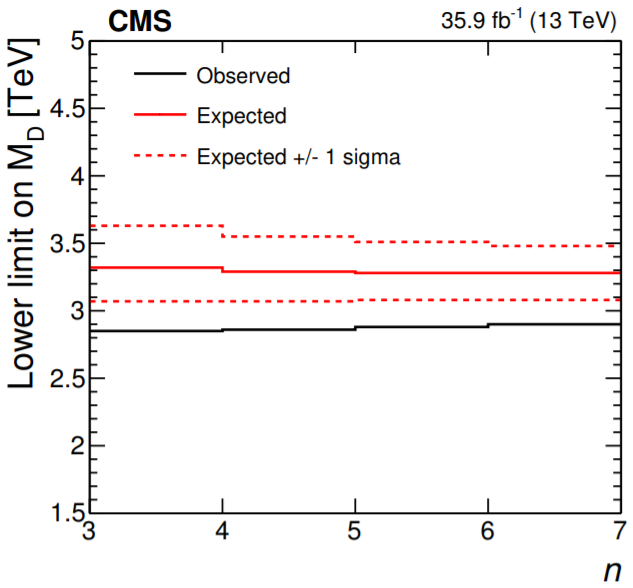
\includegraphics[width=0.42\textwidth]{Figures/add.pdf}
    \caption{
      Diagram illustrating ADD graviton emission resulting in a monophoton signature.
    }
    \label{fig:add_diagram}
  \end{center}
\end{figure}

\subsection{Previous searches} \label{sec:introduction_ADD_previous_searches}
For distances $r$ much larger than $R$, the effective gravitational potential in the ADD model has the $1/r$ form proposed by Isaac Newton (in the weak-field limit).
However, for $r \ll R$, the Newton's law potential is multiplied by $(R/r)^{n}$, leading to significant deviations from Newtonian gravitational behavior.
If $\mD \approx 1\unit{TeV}$ and $n = 1$, then to reproduce the observed value of \mPl, $R$ must be \textasciitilde$10^{13}\unit{cm}$, which
would result in noticeable differences in the orbits of the planets~\cite{ref:S0370-2693(98)00466-3}. The case $n = 2$ is disfavored by precision
measurements of Newton's law over distances on the order of 0.1\unit{mm}~\cite{ref:0264-9381/32/3/033001}.

As in the case of the aTGC model, collider limits
become strictly more stringent with increases in collider energy, starting from the LEP and moving up through the Tevatron to the LHC.
Representative curves from each of these are shown in Fig.~\ref{fig:add_noncollider_comparison}, which also shows that collider limits
on \mD\ dominate noncollider limits for $n \geq 3$. As with the DM simplified models, the strongest mono-X limits on the ADD model come from
the mono-$j/V$ channel, while the monophoton channel is the second most sensitive. The most stringent mono-$j/V$ limits from CMS exclude the ADD model
at 95\% CL for \mD\ up to 9.9\unit{TeV} when $n = 2$, and for \mD\ up to 5.3\unit{TeV} when $n = 6$~\cite{ref:PhysRevD.97.092005}.

\begin{figure}[hbtp]
  \begin{center}
    \includegraphics[width=0.90\textwidth]{Figures/add_noncollider_comparison_jpeg.jpg}
    \caption{
      Comparison of collider and noncollider limits on ADD model parameters, as shown in~\cite{ref:0264-9381/32/3/033001}.
      The marked points are monojet limits from the LEP~\cite{ref:9789812702227_0266}, Tevatron~\cite{ref:PhysRevLett.101.181602}, and LHC~\cite{ref:j.physletb.2011.10.006, ref:PhysRevLett.110.011802, ref:0264-9381/32/3/033001}.
      The Irvine~\cite{ref:PhysRevD.32.3084, ref:PhysRevLett.44.1645}, Washington~\cite{ref:PhysRevLett.98.021101}, and Stanford~\cite{ref:PhysRevD.78.022002} curves come from direct measurements of Newton's law.
      The Casimir curve~\cite{ref:0264-9381/32/3/033001} synthesizes of a range of  experimental results that constrain the existence of strong gravity using the Casimir force,
      and the pbar-HE curve~\cite{ref:epjconf/20146605021, ref:0264-9381/32/3/033001} comes from analyses of electron double scattering and exotic atom spectroscopy.
      The ADD model is excluded at 95\% CL or more in the shaded region.
    }
    \label{fig:add_noncollider_comparison}
  \end{center}
\end{figure}

Prior to the analysis presented in this thesis, the most stringent ADD limits in the monophoton final state were set in the last published results from CMS,
based on 12.9\fbinv\ of data collected in the first half of 2016~\cite{ref:JHEP10(2017)073}. The ADD model was excluded at 95\% CL for \mD\ up to 2.31\unit{TeV}
for $n = 3$, climbing to 2.49\unit{TeV} at $n = 6$, as shown in Fig.~\ref{fig:add_cms_earlylimits_MD}.

\begin{figure}[hbtp]
  \begin{center}
    \includegraphics[width=0.50\textwidth]{Figures/add_cms_earlylimits_MD.pdf}
    \caption{
    ADD limits based on CMS data from the first half of 2016 analyzed in the monophoton channel, as shown in~\cite{ref:JHEP10(2017)073}.
    Limits from the previous CMS monophoton analysis of 8\unit{TeV} data~\cite{ref:j.physletb.2016.01.057} are also shown.
    The ADD model for a given $n$ (specified by the left edge of each bin) is excluded at 95\% CL or more for \mD\ below the curves.
    }
    \label{fig:add_cms_earlylimits_MD}
  \end{center}
\end{figure}

None of these analyses report any significant evidence of BSM physics.

\chapter{The CMS experiment and the LHC} \label{chap:LHCCMS}
\section{The LHC} \label{sec:LHCCMS_LHC}
The Large Hadron Collider (LHC)~\cite{ref:1748-0221/3/08/S08001} at CERN is, as the name suggests, the world's largest
and most powerful particle accelerator. It is used to collide protons as well as heavy ions, which are both examples of hadrons, hence the ``HC'' in LHC.
Experiments attached to the collider examine the collision debris, from which features of the
parent hard-scattering process may be inferred, allowing models such as those described in Chap.~\ref{chap:introduction} to be tested.

The collider consists of a closed loop of beam pipes, along with its RF cavities (sec.~\ref{sec:LHCCMS_LHC_proton_acceleration}), magnets,
and cryogenic and vacuum systems. It sits in a circular tunnel 26.7\unit{km} in circumference, lying between 45 and 170\unit{m} underground, straddling
the French--Swiss border near Geneva, Switzerland. The beam pipes are subdivided into eight straight and eight arc sections, forming a rounded octagon.
To orient navigation, there are eight designated points spaced evenly around the tunnel perimeter, one in the middle of each 8528\unit{m}-long straight section.
The four main LHC experiments surround the LHC beam pipe at four of these points: ATLAS~\cite{ref:10.1088/1748-0221/3/08/S08003}
at point 1, ALICE~\cite{ref:1748-0221/3/08/S08002} at point 2, CMS~\cite{ref:1748-0221/3/08/S08004} at point 5, and LHCb~\cite{ref:1748-0221/3/08/S08005} at point 8.
Their arrangement is shown in Fig.~\ref{fig:LHC_schematic}.

\begin{figure}[hbtp]
  \begin{center}
    \includegraphics[width=0.70\textwidth]{Figures/Schematic-layout-of-the-LHC-at-CERN.png}
    \caption{
    Schematic layout of the LHC, from~\cite{ref:PhysRevAccelBeams.20.091002}.
    }
    \label{fig:LHC_schematic}
  \end{center}
\end{figure}

The eight arc sections are each filled with a series of dipole bending magnets, 1232 in all. These produce a uniform magnetic field in a fixed direction when a current is run through them.
A magnetic field causes a charged particle's trajectory to bend, and the dipoles are arranged so as to keep the proton beam trajectories aligned with the LHC beam pipes.
Since a fixed magnetic field causes protons moving in opposite directions to bend in opposite directions, the two counter-rotating beams must be deflected by oppositely-aligned fields.
A special two-in-one magnet design was developed for the LHC that produces two side-by-side dipole fields, coupled to the same current, oriented in opposite directions. The use of
superconducting NbTi cables allows more than 12\unit{kA} to flow when the wire is cooled to 1.9\unit{K}, producing a dipole field of up to 9\unit{T}. Sophisticated cryogenic and power
transmission systems are required to operate the magnets at this level, and the two-in-one design prevents each pipe from needing its own separate system along more than 18\unit{km} of
total dipole magnet length, substantially reducing the space and cost requirements of the LHC.

The arc dipoles each have a radius of curvature $R = 2.804\unit{km}$. This radius constrains the energy of a relativistic particle
bent in a circular trajectory by a magnetic field of magnitude $B$, via the relation~\cite{ref:WilleAccelerators}
\begin{equation}
E = qcBR
\end{equation}
where $q$ is the particle's electric charge and $c$ is the speed of light. For a fixed
particle type and magnet strength, $E$ is directly proportional to $R$. Accordingly, higher-energy
colliders tend to be built with larger circumferences than lower-energy colliders.
The energy of a fully-accelerated LHC proton in 2016 was 6.5\unit{TeV}, corresponding to a dipole field of 7.7\unit{T}.

Smaller accelerators including the Proton Synchrotron (PS) and Super Proton Synchrotron (SPS) used to be flagship accelerators
in their own right, but now chiefly serve as intermediate stages in an accelerator complex that feeds the LHC.
The LHC itself occupies the tunnel originally dug to house the Large Electron-Positron (LEP) collider~\cite{ref:SchopperLEP}, which collided
electrons and their antipartners (positrons) and ran from 1989 until 2000, setting some of the original results
listed in Chap.~\ref{chap:introduction}. The Fermilab Tevatron~\cite{ref:TevatronPhysics}, which ran from 1983 to 2011, occupied a smaller tunnel
but achieved higher energies than LEP by accelerating heavier particles: protons and their antipartners\footnote{These and other recent collider
experiments are reviewed in~\cite{ref:PDG}, chapter 30.}. The LHC, inaugurated in 2008,
accelerates protons in the world's largest accelerator tunnel, with state-of-the-art bending
magnets, allowing it to achieve unprecedented particle collision energies.

\subsection{Proton acceleration and collision} \label{sec:LHCCMS_LHC_proton_acceleration}
In practice, a low-energy proton beam is too wide to inject directly into the LHC beam pipes, but the beam can be narrowed by accelerating it~\cite{ref:PartPhysLHCEra}.
The beam is therefore passed through a chain of several different accelerators before ultimately arriving at the LHC.
Protons are initially collected by ionizing hydrogen gas, and as of 2016 they are fed to the LINAC2, a linear accelerator which accelerates
them to 50\unit{MeV} before sending them to the PS booster, which brings them up to 1.4\unit{GeV}. The protons are then sent to the PS, taking them to 25\unit{GeV},
and after that to the SPS, which pushes them to 450\unit{GeV} before finally injecting them into the LHC for final acceleration up to 6.5\unit{TeV}.

Protons are accelerated by passing through radio-frequency (RF) cavities, which generate oscillating electromagnetic
fields. Forward acceleration only results if the proton passes through the RF cavity at an opportune point in its oscillation cycle.
Thus, rather than circulating in a continuous beam, protons are segregated into discrete \textit{bunches}. In the LHC, the RF
frequency is tuned to 400.790\unit{MHz}, and bunches are spaced so as to keep 10 RF oscillations between each bunch. This corresponds
to a minimum bunch separation of 24.95\unit{ns} in time, with enough length in the tunnel to fit exactly 3564 bunches, each orbiting
with a frequency $f_\mathrm{rev} = 11.245\unit{kHz}$. A maximum of
2808 bunches can be injected in practice, to allow a sufficiently long empty interval for the beam injection and beam dump
redirector magnets to activate, and also respecting constraints imposed by assembling the bunch trains via the accelerator chain.
Beam optimization strategies and other operational constraints, including a persistent vacuum leak in the SPS beam dump
during 2016, can reduce this further. In 2016, the typical number of bunches per beam $n_b$ was 2076.

Two separate bunch trains counter-rotate around the LHC in separate beam pipes, with their paths crossing at four collision points
corresponding to each of the main experiments. The center-of-mass collision energy of the beams, $\sqrt{s}$, is twice that of the
individual beam energies. For a single-beam energy of 6.5\unit{TeV}, this corresponds to $\sqrt{s} = 13\unit{TeV}$.
Each bunch contains many billions of protons: in 2016, the typical number of protons per bunch at the start of each fill, $N_b$, was $1.25 \times 10^{11}$.
As a consequence, many pairs of protons can undergo hard collisions within the same
bunch crossing, depending on the instantaneous luminosity $\mathcal{L}$ and the total inelastic \Pp\Pp\ scattering cross section $\sigma_\mathrm{inel}$.
In 2016, there were on average 23 of these \textit{pileup} collisions per bunch crossing.

Various parameters describing the geometric profile of the bunches
are listed in Table~\ref{tab:beam_geo}. These determine $\mathcal{L}$ at the collision points, via
\begin{equation}
\mathcal{L} = \frac{N_{b}^{2}n_{b}f_\mathrm{rev}\gamma_{r}}{4\pi\epsilon_{n}\beta^\mathrm{*}}\left(1 + \frac{\theta_{c}^{2}\sigma_{z}^{2}\gamma_{r}}{4\epsilon_{n}\beta^\mathrm{*}}\right)^{-1/2}
\label{eq:instantaneous_lumi}
\end{equation}
in which the relativistic factor $\gamma_{r} = E_\mathrm{beam}/m_{p}$ has a value of 6930 for $E_\mathrm{beam} = 6.5\unit{TeV}$.
The value of $\mathcal{L}$ corresponding to the typical 2016 parameter values listed above is $1.3 \times 10^{34}$ $\mathrm{cm}^{-2}\mathrm{s}^{-1}$.

\begin{table}
\centering
\begin{tabular}{ cc }
\hline
Normalized transverse emittance $\epsilon_{n}$ & 3.4\unit{\micro m} \\
$\beta^{*}$ & 40\unit{cm} \\
Crossing angle $\theta_{c}$ & 185\unit{\micro rad} \\
RMS longitudinal bunch length $\sigma_{z}$ & 7.87\unit{cm} \\
\hline
\end{tabular}
\caption{Beam geometry parameters for 2016}
\label{tab:beam_geo}
\end{table}

\subsection{Collimation, magnets, and beam halo} \label{sec:LHCCMS_LHC_magnets_beam_halo}
The beams can lose protons during transit through a variety of mechanisms, such as intra-beam scattering
and scattering off of residual gas inside the tunnel~\cite{ref:1748-0221/3/08/S08001}. Among other consequences, this leads
to the accumulation of a ``halo'' of protons with large radial separation from the central beam axis, accompanying the main beam.
If left unchecked, beam halo could damage unprotected equipment and leave spurious signals in detectors.
Furthermore, if a bending magnet were to suddenly fail, the beam would sweep across the area downstream of the magnet, dumping a potentially
devastating load of radiation on whatever it hit.

Collimators stationed around the beam line capture and remove this halo,
and additionally protect the LHC and its detectors from sudden beam control failure.
Every proton--collimator interaction produces a residual shower of secondary particles that emerge from the other side of the collimator
and continue forward, so a series of several collimators is required.
Primary LHC collimators (TCP) clean the beam at Points 3 and 7, and secondary collimators (TCS) catch most of the output from those.
Tertiary collimators (TCT) made of a heavy tungsten alloy sit on either side of the CMS experimental cavern,
to scrub as much remaining halo as possible before it reaches the detector~\cite{ref:PhysRevAccelBeams.20.091002}.

As noted above, a series of 1232 main dipole magnets spaced around the LHC keep the beams moving
in their quasi-circular trajectories around the tunnel. A multitude of other magnets serve more specialized roles. Quadrupole
magnets have the effect of squeezing the beam along one axis and stretching it along another, and are used to focus
the beam along a specific direction. Near the interaction point (IP) of each experiment, an inner triplet of quadrupole magnets
are the last to interact with the beams before they collide. Figure~\ref{fig:magnet_positions} shows the arrangement
of magnets near the ATLAS and CMS IPs.

\begin{figure}[hbtp]
  \begin{center}
    \includegraphics[width=0.80\textwidth]{Figures/magnet_positions.png}
    \caption{
    Dipole (D1-2) and quadrupole (Q1-7) magnet arrangement near the left side of the IP, from~\cite{ref:PAC.2003.1289077}.
    This arrangement is mirrored on the right side of the IP.
    The figure specifically designates IP1, the ATLAS IP; the magnet layout is identical around IP5, the CMS IP.
    The inner triplet of quadrupole magnets (with two varieties, designated MQXA and MQXB)
    are the last to interact with the beam before collision.
    The distance from the left edge of Q3 (MQXA) to the IP is about 53\unit{m},
    and the distance from the right edge of Q1 to the IP is about 23\unit{m}.
    The TCT sits between D2 and TAN, about 150\unit{m} from the IP.
    }
    \label{fig:magnet_positions}
  \end{center}
\end{figure}

The envelope of each beam reaches a maximum in the inner triplet
before finally being focused toward a minimum at the interaction point. Beam halo is correspondingly widely dispersed,
and the TCTs are specifically placed about 150\unit{m} out from the IP so as to protect the inner triplet from this halo~\cite{ref:PhysRevSTAB.18.061001}.
Secondary particles produced from beam
halo collisions with the TCTs include large numbers of high-energy muons, along with an assortment of other secondaries.
These, along with the secondaries from proton collisions with residual gas in the beam pipe, comprise
what is called the machine-induced background (MIB) impinging on CMS~\cite{ref:1748-0221/10/11/P11011}.

In contrast to protons in the beam, secondary muons are neither narrowly nor evenly focused by the final stretch of magnets before reaching the IP.
They enter the CMS cavern traveling parallel to the beam pipe with a wide radial profile, often having a high enough
radius to hit the exterior muon chambers and calorimeters~\cite{ref:1748-0221/10/11/P11011}.
Furthermore, the transverse distribution of MIB (Fig.~\ref{fig:beamhalo_sim}) is highly anisotropic, concentrating near the
horizontal plane.

\begin{figure}[hbtp]
  \begin{center}
    \includegraphics[width=0.50\textwidth]{Figures/beamhalo_sim.png}
    \caption{
    Simulated distribution of MIB flux transverse to the beam pipe in the CMS cavern,
    20.6 m from IP5. From~\cite{ref:1748-0221/10/11/P11011}. The $x$ and $y$ coordinates
    are defined in sec.~\ref{sec:LHCCMS_CMS_coordinates}.
    }
    \label{fig:beamhalo_sim}
  \end{center}
\end{figure}

\section{The CMS experiment} \label{sec:LHCCMS_CMS}
The CMS, short for Compact Muon Solenoid, is a general-purpose particle detector surrounding the LHC beam pipe
centered at IP5, located 100\unit{m} underground near Cessy, France. Multiple layers of metal absorbers, crystal and plastic scintillators,
and electrically-tensed gas chambers and silicon semiconductors are arranged so as to interact with different types of particles in discernably different ways.
Millions of sensors collect fine-grained information on the interactions of particles
within these layers, and the resulting data is used to precisely reconstruct the type, charge, energy, momentum, and trajectory
of nearly every final-state particle emerging from a hard collision event.

A broad overview of the experiment is shown in Fig.~\ref{fig:cms_annotated}.
A more comprehensive description is given in~\cite{ref:1748-0221/3/08/S08004}, the reference from which much of the material in this section derives.
The CMS is a dynamically-evolving apparatus, responding to changing experimental conditions and advances in detection technology and methods.
The description of CMS given in this section specifically applies to its setup in 2016, the year in which collision data for this thesis was taken.

\begin{figure}[hbtp]
  \begin{center}
    \includegraphics[width=0.99\textwidth]{Figures/cms_annotated.png}
    \caption{
    A schematic illustration of the CMS experiment, with one octant cut away for visibility.
    }
    \label{fig:cms_annotated}
  \end{center}
\end{figure}

\subsection{Coordinate system} \label{sec:LHCCMS_CMS_coordinates}
The coordinate system is centered at IP5, the nominal interaction point inside the CMS experiment.
The positive $x$-direction points radially inward toward the center of the LHC ring, the positive $y$-direction
points vertically upward, and the positive $z$-direction is oriented counterclockwise around the LHC when viewed
from above, as in Fig.~\ref{fig:cms_coordinates}.
The radial coordinate in the $x$--$y$ plane is denoted $r$, and the azimuthal angle $\phi$ is measured counterclockwise
(viewed from the positive $z$-direction, looking toward the negative $z$-direction) from the $x$-axis in this plane.
The polar angle $\theta$ is measured from the positive $z$-direction.

\begin{figure}[hbtp]
  \begin{center}
    \includegraphics[width=0.90\textwidth]{Figures/cms_coordinates.pdf}
    \caption{
    The CMS coordinate system.
    }
    \label{fig:cms_coordinates}
  \end{center}
\end{figure}

The \textit{longitudinal momentum} of a particle is defined as the component of its momentum along the $z$-axis, with
magnitude $p_\mathrm{L}$. The \textit{transverse momentum} of a particle is the component of its momentum perpendicular
to the longitudinal momentum, lying in the $x$--$y$ plane,
and can be specified by its magnitude \pT\ and its direction $\phi$.

Hard \Pp\Pp\ collisions
result in the interaction of individual partons, each of which can carry different fractions of their
parent \Pp\ momentum. Even if the longitudinal momenta of the colliding protons are perfectly matched,
the longitudinal momenta of the interacting partons may not be. However, the \pT\ of
both parent protons is negligible, and any fraction of zero is still zero. There is some small
\pT\ spread of partons within a proton, but in general, the \pT\ of colliding partons is almost exactly zero, within the limits of detector sensitivity.

By the law of conservation of momentum, the vector sum of the
transverse momenta of all collision products must therefore sum to zero. However, the sum of the longitudinal momenta
can vary appreciably, as can the net longitudinal velocity of the collision event. According
to the theory of special relativity, differences in $\theta$ between events will appear different
to different observers depending on their relative longitudinal velocity. In other words, differences in $\theta$ are not Lorentz invariant.

Differences in a related quantity called the \textit{rapidity}, defined as
\begin{equation}
\mathrm{rapidity} = \frac{1}{2}\ln{\frac{E+p_\mathrm{L}}{E-p_{L}}},
\label{eq:rapidity}
\end{equation}
are Lorentz invariant. Particle production in LHC collisions is roughly constant as a function of rapidity~\cite{ref:lhcrun1harvest_ch3}, and because
differences in rapidity do not depend on the longitudinal speed at which one is moving, that statement is independent
of whether the collisions are observed in their own rest frame or in that of the CMS. At very high
energies, rapidity becomes approximatey equal to the \textit{pseudorapidity} $\eta$ defined by
\begin{equation}
\eta = -\ln{\tan{(\theta/2)}}.
\label{eq:pseudorapidity}
\end{equation}

Since $\theta$ only depends on the position of the detector component in which a particle is measured, $\eta$
serves as a convenient coordinate to describe the kinematics of high-energy \Pp\Pp\ collisions in a Lorentz-invariant way.
Pseudorapidity begins at 0 for particles emitted from the IP exactly perpendicular to the beam, and rises in magnitude for particle
trajectories more closely aligned with the beam axis, diverging to infinity as $\theta$ approaches 0. A particle may be considered ``isolated''
or well-separated from other particles in a collision event if there is little excess activity in a given $\Delta R$ cone surrounding
the particle, where
\begin{equation}
\Delta R = \sqrt{\Delta\eta^{2} + \Delta\phi^{2}}
\label{eq:deltaR}
\end{equation}

The CMS has approximately hermetic coverage of particles emerging from the IP with $|\eta|$
up to 5.0, giving a total polar coverage of 178.46 degrees along with complete 360-degree azimuthal coverage. Particles emerging
within this zone of coverage are detected with high probability by at least one subsystem, although the measurement quality varies
as a function of $|\eta|$. Since particles are emitted with a roughly constant concentration as a function of $\eta$, and because
cones of constant $\eta$ become more densely packed at higher values of $|\eta|$, it follows that the intensity of particle radiation
impinging on detector elements is stronger at higher $|\eta|$. Tradeoffs must be made between the measurement quality of an apparatus
and its radiation hardness, and therefore equipment installed at higher $|\eta|$ is typically less precise.

\subsection{Superconducting solenoid and silicon tracking system} \label{sec:LHCCMS_CMS_magnet_tracker}
The ``S'' in CMS derives from the 12.5-m-long, 0.3-m-thick, 6-m-inner diameter solenoid surrounding the core of the experiment.
When an 18 kA current is applied to its more than 2000 windings of superconducting cable, it produces a homogeneous 3.8\unit{T} magnetic
field in its center. The field is returned in the opposite direction with about half the magnitude by an iron return yoke surrounding
the solenoid, consisting of three barrel layers split into five wheels, complemented by three endcap disk layers at each end.

The size and shape of the solenoid are a primary design constraint for CMS. The HCAL, ECAL, and inner tracker together must be compact
enough to fit completely inside it, giving rise to the ``C'' in CMS. Because of the cylindrical shape of the solenoid,
all primary detector layers in CMS are divided into cylindrical barrel sections complemented by flat circular endcaps on either end.

The magnetic field produced by the solenoid is illustrated in Fig.~\ref{fig:solenoid_field}.
Charged particles traveling through this field have their trajectories bent, and at 3.8\unit{T} the field will noticeably
bend even very high-momentum particles. This allows the ratio of a particle's momentum to its charge to be measured, as particles
with higher momentum are bent less than particles with the same charge but lower momentum. It also allows the sign of a particle's electrical charge
to be identified, as positively- and negatively-charged particles are bent in opposite directions (and electrically neutral
particles are not bent at all).

\begin{figure}[hbtp]
  \begin{center}
    \includegraphics[width=0.90\textwidth]{Figures/solenoid_field.png}
    \caption{
    Magnetic field produced by the CMS solenoid, from~\cite{ref:1748-0221/5/03/T03021}. The field strength in T is shown on the left,
    and contour lines smoothly connecting the field direction are shown on the right.
    }
    \label{fig:solenoid_field}
  \end{center}
\end{figure}

The trajectories of charged particles close to the IP are mapped by an inner silicon tracking system, the innermost detector layer of CMS.
It is based on tracking elements made from radiation-hard silicon, allowing high-speed measurements.
Charged particles passing through the silicon tracker elements release bursts of free electric charge in the silicon. An applied voltage causes
the charge to migrate to a detector at the edge of the element, allowing it to infer the time and location of the hit.
Fine-grained position and time resolution is obtained by subdividing the tracker volume into tens of millions of separate tracking detector elements
spread over multiple layers. Figure~\ref{fig:inner_tracker} illustrates the arrangement of tracker layers.

\begin{figure}[hbtp]
  \begin{center}
    \includegraphics[width=0.99\textwidth]{Figures/tracker_schematic.png}
    \caption{
    Arrangement of layers in the inner tracker.
    }
    \label{fig:inner_tracker}
  \end{center}
\end{figure}

The inner tracker is subdivided into a pixel tracker surrounded by a strip tracker. The pixel tracker is the first CMS module that
low-$|\eta|$ ($\lesssim 2.5$) particles pass through. It is subdivided into three barrel layers at $r = 4.4$, 7.3, and 10.2\unit{cm},
and two endcap disks on each side at $|z| = 34.5$ and 46.5\unit{cm}. These layers are arranged so that at least three are hit by
any particle with $|\eta| < 2.5$.
The tracking elements comprise 66 million pixels, 48 million in the barrel layers
and 18 million in the endcap disks, each with an area of $100{\times}150\unit{\micro m}^{2}$.

The strip tracker is subdivided into an inner barrel (TIB), inner disks (TID), outer barrel (TOB), and endcaps (TEC).
The TIB consists of four cylindrical layers, capped by the TID which comprises three circular disks on each side of TIB.
Together, TIB and TID extend from $r = 20\unit{cm}$ to 50\unit{cm} and out to $|z| = 90\unit{cm}$.
The TOB surrounds the TIB and TID and consists of six cylindrical layers. The TEC caps both TOB and TID and comprises
nine circular disks on each side, complementing the TOB's radial coverage out to $r = 114\unit{cm}$ and extending the $|z|$ coverage
to 280\unit{cm}. The inner radius of TEC tapers upward with increasing radius so as to approximately adhere to the line $|\eta| = 2.5$.
All together, the tracking elements comprise 9.3 million silicon strips, each with an area of $80{\times}180\unit{\micro m}^{2}$.

Both the pixel and strip trackers have hermetic coverage up to $|\eta| = 2.5$. Charged particles with $|\eta|$ in this range will
tend to leave deposits in multiple layers of the inner tracker. By linking these sequential deposits together, the particle's trajectory through the inner
tracker may be inferred.

\subsection{Electromagnetic calorimeter} \label{sec:LHCCMS_CMS_ECAL}
The electromagnetic calorimeter (ECAL) is the second main detector layer, after the inner tracker. It comprises $75\,848$ lead tungstate ($\mathrm{PbWO}_{4}$)
crystals, divided among a cylindrical barrel section (EB) and two endcap sections (EE). The overall structural organization of the ECAL is shown in Fig.~\ref{fig:ecal_schematic}.

\begin{figure}[hbtp]
  \begin{center}
    \includegraphics[width=0.80\textwidth]{Figures/ecal_schematic.png}
    \caption{Schematic illustration of the ECAL, showing the longitudinal arrangement of crystals in the barrel and endcap sections.}
    \label{fig:ecal_schematic}
  \end{center}
\end{figure}

The barrel extends to $|\eta| = 1.479$,
and its $61\,200$ crystals are arranged in 170 wheels of 360 crystals each. Every ECAL crystal is shaped like a long, tapered rectangular prism with one
larger, exterior square face attached to a sensor, and a smaller interior square face generally pointing toward the inner tracker. Crystals in EB
are 23.0\unit{cm} long, with a $22{\times}22\unit{mm^2}$ interior face and $26{\times}26\unit{mm^2}$ exterior face. These proportions ensure
a constant coverage of approximately 0.0174 in both $\eta$ and $\phi$ along the entire length of the crystal. The center of each interior face sits at $r = 1.29\unit{m}$.
The crystals lie approximately along projective lines, i.e.\ lines directed toward the IP. To ensure fully hermetic coverage of particles leaving the IP,
they are tightly packed with 0.35--0.50\unit{mm} of separation between adjacent crystals, and are tilted by 3 degrees off of the true projective line.

The remainder of the ECAL comprises two endcap disks of 7324 crystals each, covering $1.479 < |\eta| < 3.0$.
Crystals in EE are each 22.0\unit{cm} long with a $28.6{\times}28.6\unit{mm^2}$ interior face and $30{\times}30\unit{mm^2}$ exterior face.
The rectangular crystals are stacked in an approximation of a circle. They point along projective lines, directed not at the IP, but rather at a point on
the beam axis 1.3\unit{m} past the IP. The interior edges of EE sit at $|z| = 315.4\unit{cm}$ when the experiment is running\footnote{The intense magnetic
field of the solenoid measurably constricts the CMS detector apparatus, pulling in EE by an estimated 1.6\unit{cm}.}.

Lead tungstate crystal is a scintillator, producing visible
light in the range of 430\unit{nm} (blue-green) in response to the passage of photons and electrons. The blue-green scintillation light travels freely through
the optically transparent crystal, and sensors affixed to the outer face of each crystal collect this light. While its light output is not as high as some other
scintillators (at maximum crystal transparency, about 4.5 electrons per incident MeV are collected by the sensors), $\mathrm{PbWO}_{4}$ was the material of choice
due to its high radiation tolerance, short radiation length ($X_{0} = 0.89\unit{cm}$), and small Molière radius (2.2\unit{cm}).

High-energy electrons (or antielectrons) passing through a high atomic number material such as Pb or W will tend to lose energy in discrete
bursts via the emission of photons (a phenomenon called \textit{bremsstrahlung}, ``braking radiation''), and high-energy photons will tend to propagate freely until suddenly decaying into
an electron--antielectron ($e^{+}e^{-}$) pair. The \textit{radiation length} $X_{0}$ is both the mean distance over which an electron has its energy reduced by bremsstrahlung
by a factor of $1/e$, as well as $7/9$ of the mean free path for photons before they convert to an $e^{+}e^{-}$ pair.

The products of a photon conversion are themselves high-energy electrons and antielectrons, and bremsstrahlung photons tend to have high energies as well,
resulting in a stochastic sequence of photon emissions and $e^{+}e^{-}$ pair production events called an \textit{electromagnetic shower}. As the shower
propagates through a given material, it spreads outward in a roughly conical shape with a characteristic average width. The \textit{Molière radius} of a material
is defined to be the radius of a cylinder, aligned with an electromagnetic shower, encompassing an average of 90\% of the shower's energy.

By conservation of energy, the total shower energy is the same as the energy of the original $e$ or $\gamma$, and by conservation of momentum,
the mean direction of the shower is also the same as that of the original $e/\gamma$. The long depth of the crystals relative to their radiation
length---25.8 $X_{0}$ in EB, 24.7 $X_{0}$ in EE---ensures that nearly 100\% of incident $e/\gamma$ stemming
from \Pp\Pp\ collisions leave electromagnetic showers that are fully contained by the ECAL, allowing their energies to be reliably inferred.
The small Molière radius of $\mathrm{PbWO}_{4}$ allows their orientation to be accurately judged, and nearby showers can be reliably separated in most cases.

The scintillation light is collected in EB crystals by avalanche photodiodes (APDs), and in EE crystals by more radiation-tolerant
vacuum phototriodes (VPT). The amount of light collected is directly proportional to the shower energy contained in the crystal.
The time of arrival of the shower is inferred by fitting a pulse shape to input signals collected every 25\unit{ns}. It takes time for the
crystal scintillation to fully die down---after 25\unit{ns}, about 80\% of the total scintillation light has been emitted---so the full pulse shape
is spread over more than one input.

Free neutrons produced in the calorimeters can migrate through the detector and interact with a layer of epoxy used to affix the APD
to the crystal surface, ejecting protons directly into the APD active volume. This triggers the release of thousands of electrons into the APD,
resulting in a spurious signal that can be mistakenly reconstructed as an $e/\gamma$ deposit with very high energy~\cite{ref:1742-6596/404/1/012043}.
Since these \textit{spikes} occur in single crystals, most can be distinguished from real $e/\gamma$ showers by their narrow distribution of shower energy,
as illustrated in Fig.~\ref{fig:spike_energy_distribution}.
The APD does not receive a continuous light signal from the crystal scintillation in these events, so the pulse shape is constructed from
only one input signal, as illustrated in Fig.~\ref{fig:spike_pulse_shape}. This has the net effect of shifting the inferred time of arrival backward, and most spikes have a measured arrival time between 10 and 15\unit{ns}
before real photons in a given bunch crossing. ``Double spikes'' involving two neighboring crystals have also been observed, presumably
arising from a secondary nucleon ejected by the primary neutron. These are similarly distinguishable from real $e/\gamma$ showers by their narrow
energy distribution and early arrival time.

\begin{figure}[hbtp]
  \begin{center}
    \includegraphics[width=0.49\textwidth]{Figures/real_egamma_energy_distribution.png}
    \includegraphics[width=0.49\textwidth]{Figures/spike_energy_distribution.png}
    \caption{Distributions of electromagnetic shower energy among neighboring ECAL crystals. The distribution from an actual
    $e/\gamma$ shower is shown on the left, and a spike distribution is shown on the right. From~\cite{ref:spikes_farzanehfar}.}
    \label{fig:spike_energy_distribution}
  \end{center}
\end{figure}

\begin{figure}[hbtp]
  \begin{center}
    \includegraphics[width=0.60\textwidth]{Figures/spike_pulse.png}
    \caption{Pulse shapes in the APD produced by spikes and by genuine electromagnetic showers, from~\cite{ref:DN-2015/014}.}
    \label{fig:spike_pulse_shape}
  \end{center}
\end{figure}

Neutral pions (a type of hadron produced copiously in \Pp\Pp\ collisions) decay rapidly into two photons,
and when the pion is traveling at high speed, these photons will emerge moving in very close to the same direction.
Despite the relatively small Molière radius of $\mathrm{PbWO}_{4}$, it can still be difficult to discern whether the ECAL
has been struck by a single high-energy photon or two tightly-collimated photons from a pion decay.
To facilitate the identification of these pions, a preshower detector is installed on the EE.

The preshower comprises two modules, one attached to the inner edge of each ECAL endcap. A module consists of two layers,
each with a lead radiator followed by a silicon strip sensor, and has a total thickness of 20\unit{cm}, covering $1.653 < |\eta| < 2.6$.
The inner lead layer initiates electromagnetic showers from incoming $e/\gamma$ particles,
and the silicon sensor behind it measures the shower shape and energy.
The second layer of lead continues the shower evolution, and the second layer of sensors provides another measurement.
This is an example of a sampling calorimeter, and the same general strategy is employed by HCAL, described in the following section.

\subsection{Hadronic calorimeter} \label{sec:LHCCMS_CMS_HCAL}
After the ECAL, the next layer a particle will encounter is the hadron calorimeter (HCAL)\footnote{If the particle has $|\eta| > 3.0$,
the forward portion of HCAL is the first and only CMS detector layer it hits.}.
The HCAL is subdivided into three main systems: the barrel (HB), endcap (HE), and forward calorimeters (HF).
Figure~\ref{fig:hcal_schematic} shows their overall layout.

\begin{figure}[hbtp]
  \begin{center}
    \includegraphics[width=0.90\textwidth]{Figures/hcal_layout.png}
    \caption{
    Schematic illustration of the HCAL overlaid with dashed lines of constant $\eta$, from~\cite{ref:1748-0221/3/08/S08004}.
    Indicative arrangements of the muon systems, solenoid, ECAL, and inner tracker are also shown.
    }
    \label{fig:hcal_schematic}
  \end{center}
\end{figure}

The barrel and endcap systems are sampling calorimeters with alternating layers of brass absorber and plastic scintillator.
The brass in the absorbers is an alloy of 70\% Cu and 30\% Zn. High-energy hadrons hitting the nuclei in these atoms can eject
a number of secondary hadrons, which themselves can eject further hadrons in a cascade known as a \textit{hadronic shower}.
Like electromagnetic showers, hadronic showers have a characteristic length, the \textit{nuclear interaction length} $\lambda_{I}$.
Hadrons such as pions can also decay midflight into high-energy $e/\gamma$, leading to secondary electromagnetic showers.
The brass absorbers have $\lambda_{I} = 16.42\unit{cm}$ and $X_{0} = 1.49\unit{cm}$.

Absorber layers are interleaved with plastic scintillator tiles, with about 70\,000 in total distributed between HB and HE.
Inlaid fiber optic cables sample the scintillation light and carry it to hybrid photodiode (HPD) sensors. Up to 17 layers of
plastic scintillator are stacked against each other in HB and HE, interleaved by brass absorber layers.

The barrel section covers $|\eta| < 1.3$.
Layers of HCAL scintillators and absorbers lie parallel to the beam line. Towers of related scintillator tiles are grouped along
projective lines pointing toward the IP, as shown in Fig.~\ref{fig:hcal_towers}.
In HB there are 16 tower divisions in $\eta$ on either side of $\eta = 0$, and 72 tower divisions in $\phi$, such that each tower
has an $\eta$--$\phi$ coverage of $0.087{\times}0.087$. The brass and scintillator layers are separated into wedges in $\phi$.
So as to ensure hermetic coverage throughout HB, the brass layers within each wedge are staggered, and adjacent wedges are separated by less than 2\unit{mm}.

\begin{figure}[hbtp]
  \begin{center}
    \includegraphics[width=0.75\textwidth]{Figures/hcal_towers.png}
    \caption{
    Arrangement of HB, HE, and HO towers, from~\cite{ref:1748-0221/3/08/S08004}.
    }
    \label{fig:hcal_towers}
  \end{center}
\end{figure}

The effective thickness of HB ranges from 5.39 $\lambda_{I}$ at tower 0 to 10.3 $\lambda_{I}$ at tower 15; tower 16 partially overlaps with HE.
About 1.1 additional $\lambda_{I}$ are supplied by the ECAL. The thickness of HB is constrained by the available space between EB
and the solenoid. In order to provide a more robust measurement of shower energy, and also to supply additional insulation to the outer muon systems
by capturing hadrons exiting the rear of HB, HCAL is supplemented by an outer barrel layer (HO) directly behind the solenoid.
The solenoid itself contributes about 1.4 $\lambda_{I}$ at low $|\eta|$.

The endcaps cover $1.3 < |\eta| < 3.0$. Like HB, the layers in HE are staggered so as to provide hermetic coverage. Unlike HB,
no additional outer layer is needed, since HE is about 10 $\lambda_{I}$ thick over its entire span. Towers in EE have a coverage
of $0.087{\times}0.087$ for $|\eta| < 1.6$ and approximately $0.17{\times}0.17$ for $1.6 < |\eta| < 3$.

The HF covers the forward region, $3 < |\eta| < 5$. It is composed mostly of steel with embedded quartz fiber, built in a cylindrical shape with a radius of 130.0\unit{cm}.
The cylinder's inner face sits 11.2\unit{m} from the IP and it extends 165\unit{cm} longitudinally, supplying approximately 10 $\lambda_{I}$ for
the development of hadronic showers. The intense radiation in the forward region necessitated the use of quartz fibers as the active medium for shower energy probing.
High-energy charged particles in these showers generate Cherenkov light as they pass through the fibers, which run from front to back through the cylinder,
and serve as fiber optic cables carrying that light to photomultiplier tubes. Half of the fibers run over the full length of the
steel cylinder, and the other half begin 22\unit{cm} back from the inner face, allowing $e/\gamma$ (which deposit most of their energy in the first 22\unit{cm}) to be
distinguished from hadrons (which deposit their energy roughly equally before and after 22\unit{cm}). The fibers are bundled in towers, each with an
$\eta$--$\phi$ coverage of $0.175{\times}0.175$. For additional radiation protection, the HF is enclosed by layers of steel, concrete, and polyethylene shielding,
up to 85\unit{cm} thick on the sides.

\subsection{Muon systems} \label{sec:LHCCMS_CMS_muon}
The ``M'' in CMS reflects the central role of muon detection and measurement in the design of the experiment.
High-energy muons are minimum-ionizing particles (MIPs), reaching the outer muon systems largely unaffected by their passage through
the inner detector layers. In contrast, most other particles are fully absorbed by more than 16 $\lambda_{I}$ of material in the inner
layers, leaving a relatively background-free environment in the muon chambers.

The muon chambers interleave the steel flux-return yoke, which in addition to concentrating the exterior magnetic field also serves
to block other remnant particles from reaching the chambers. The layout of muon chambers is shown in Fig.~\ref{fig:muon_system}.
Like other CMS layers, the muon system is divided into a central barrel section and two endcaps. The barrel section is instrumented by four
layers of drift tube (DT) chambers, which cover $|\eta| < 1.2$. Each layer contains 8 chambers that measure the muon coordinates in the $r$--$\phi$
plane, and the inner three layers have an additional 4 chambers to measure the muon coordinate in the $z$ axis.

\begin{figure}[hbtp]
  \begin{center}
    \includegraphics[width=0.99\textwidth]{Figures/muon_system.pdf}
    \caption{
    Muon systems in a quadrant of CMS. Indicative arrangements of the solenoid, HCAL, ECAL, and inner
    tracker are also shown.
    }
    \label{fig:muon_system}
  \end{center}
\end{figure}

The endcaps, subject to higher radiation fluences and more nonuniform magnetic fields, are instrumented by four layers of cathode strip chambers (CSCs),
which cover $0.9 < |\eta| < 2.4$. Cathode strips, oriented in the radial direction, give a measurement in the $r$--$\phi$ plane, and anode
wires running perpendicular to the strips provide an additional measurement of the muon $\eta$.

During the design of CMS, the reliability of time measurements from these two systems of muon chambers was highly uncertain, and thus a third system
consisting of resistive plate chambers (RPCs) was installed. These provide a relatively coarse position measurement, but a highly
accurate time measurement. Muons with $|\eta|$ up to about 1.7 will pass through at least 4 RPC layers.

\subsection{Trigger system} \label{sec:LHCCMS_CMS_trigger}
Data readout from the detectors occurs at a rate of 40\unit{MHz} (once every 25\unit{ns}), corresponding with the LHC bunch crossing frequency.
The memory needed to store the full data produced in one collision event is about 1\unit{MB}, and
it is presently impossible to extract or store data collected at a rate of 40 million \unit{MB/s}.
Therefore, the data is first filtered through a \textit{trigger} system, which rapidly decides which events to store
and which to discard.

The trigger system proceeds in sequential levels. The Level 1 (L1) trigger uses a reduced set of detector information to make an initial,
extremely rapid (within 4\unit{\micro s}) filtering decision at the rate of 100\unit{kHz}. Meanwhile the full detector data sits in a buffer.
If the L1 accept (L1A) is given, that data is sent to the High-Level Trigger (HLT); otherwise it is discarded.
The HLT uses the full data to make a less time-intensive, more sophisticated decision. Events accepted by the HLT have their data permanently stored.

The L1 trigger consists of custom hardware connected by fiber links to the CMS muon and calorimeter systems\footnote{Information
from the inner tracker is not presently used by L1.}. Information from HCAL and ECAL is
sent through a dedicated calorimeter trigger pipeline, and information from the muon systems is sent through a separate muon trigger pipeline.
The output of both of these pipelines is evaluated by a Global Trigger (GT), which makes
the final L1A decision. The organization of L1 pipelines is illustrated in Fig.~\ref{fig:l1_trigger_pipeline}.

\begin{figure}[hbtp]
  \begin{center}
    \includegraphics[width=0.80\textwidth]{Figures/l1_trigger_pipeline.png}
    \caption{
    Schematic diagram of the L1 trigger pipeline.
    }
    \label{fig:l1_trigger_pipeline}
  \end{center}
\end{figure}

The \textit{trigger primitives} (TPs) sent by HCAL and ECAL are transverse energy sums recorded in calorimeter towers.
These along with some quality information are sent to Layer 1 of the calorimeter trigger,
which performs preprocessing, energy calibration, and the computation of some simple values. Layer 2 uses this information to construct
various physics objects---L1 Jets, Taus, and EGamma\footnote{With only calorimeter information, it is difficult to distinguish $e$ from $\gamma$.
In full offline event reconstruction, this classification is refined by incorporating inner tracker information.}---using simple and fast reconstruction algorithms.
Layer 2 comprises 9 parallel cards which analyze sequential events in a round-robin, ``time-multiplexed'' fashion, so as to give
each card adequate memory and processing time for each event. The demultiplexer (DeMux) organizes the resulting output and sorts the L1 objects by $p_\mathrm{T}$,
sending this information along to the GT.

The TPs from CSCs and DTs are track segments. Along with hits recorded in the RPCs, muon system TPs are routed through a lattice of preprocessor
layers and then sent to dedicated Barrel, Endcap, and Overlap Track Finders covering different $\eta$ regions.
These rapidly assemble L1 Muon objects and send them to the Global Muon Trigger,
which sorts the L1 Muons by $p_\mathrm{T}$ and quality, finally sending this information along to the GT.

The GT tests the L1 objects it receives against a set of L1 trigger paths, which specify various event selection criteria. After evaluating
which trigger paths have been passed, the GT makes the final L1A decision. The time from TP generation to L1A decision cannot be longer than
4\unit{\micro s}, and the overall L1A rate cannot be higher than 100\unit{kHz}; in 2016, this was the typical L1A rate actually achieved.

If the L1A is given, the full detector data is sent to the HLT, which consists of software running on commercial computing hardware.
The HLT tests each event against a set of high-level trigger paths. Each of these paths has access to raw detector information as well
as quantities computed at L1. Enough time and memory are available to perform a reduced sequence of the full offline event reconstruction
algorithms, separately optimized for each path. In 2016, the average HLT processing time per event was less than 160\unit{ms},
and the typical HLT accept rate was 1\unit{kHz}.

\subsection{Luminosity measurement} \label{sec:LHCCMS_CMS_lumi}
In principle, the integrated luminosity is given by integrating the instantaneous luminosity defined by Eq.~\ref{eq:instantaneous_lumi} over the data taking period,
with an extra efficiency factor to account for the fraction of time during which the trigger was active. In practice, the uncertainty on the
parameters of Eq.~\ref{eq:instantaneous_lumi} is fairly high, and more precise measurements of instantaneous luminosity are obtained by directly examining the beam intensities.

In the method developed
by van der Meer~\cite{ref:CERN-ISR-PO-68-31}, the two beams are scanned across each other in the transverse plane, giving a direct experimental
probe of the beam profile that is used to calibrate the relationship between instantaneous luminosity and specific observables accessible to various
beam monitoring instruments. A van der Meer scan establishes the calibrated visible cross section $\sigma_\mathrm{vis}$ of a process examined
by each luminometer, such that the instantaneous luminosity measured by a luminometer is given by
\begin{equation}
\mathcal{L} = R / \sigma_\mathrm{vis}
\label{eq:lumi_calibration}
\end{equation}
where $R$ is the observed rate of the process measured by the luminometer. The pixel tracker, DTs, and HF are used for this purpose, in addition to two
dedicated instruments: the Fast Beam Conditions Monitor (BCM1f) and Pixel Luminosity Telescope (PLT).

Van der Meer scans require dedicated LHC runs outside of normal data taking, but the calibrated luminometers continue to monitor the beam luminosity
during physics runs. The uncertainty on calibrated luminosity measurements in 2016 data taking is 2.5\%~\cite{ref:CMS-PAS-LUM-17-001}.
The data set used in this thesis corresponds to a time-integrated luminosity $L = 35.9$\,\fbinv.

\chapter{Simulation} \label{chap:simulation}
\section{Parton distribution functions} \label{sec:simulation_pdf}
A hard collision involving a proton can cause individual partons within it to be clearly resolved.
For collisions with characteristic energy $Q$, the probability that the parton will be of type $i$
and carry a fraction $x$ of the proton's total momentum is given by a function $f_{i}(x, Q^{2})$
known as a parton distribution function (PDF).

The dependence of these functions on $Q$ is described by the DGLAP equations~\cite{ref:0370-2693(71)90576-4, ref:dokshitzer, ref:0550-3213(77)90384-4},
which are derived from the theory of QCD.
These allow the specific values of $f_{i}(x, Q^{2})$ to be calculated at arbitrary $Q$ as long as they
are first measured at some particular $Q$.
Like cross sections, the DGLAP equations, and hence PDFs derived in this way, admit perturbative expansions out to specific orders in
$\alpha_\mathrm{S}$~\cite{ref:0034-4885/70/1/R02}.

Simulated samples used in this thesis use PDFs computed to different orders as appropriate for the order
of the cross section used. Samples with cross sections computed to LO in $\alpha_\mathrm{S}$ use the NNPDF3.0 LO PDF
set~\cite{ref:NNPDF30}. Samples with NLO cross sections, as well as theoretical \zinvg, \wlng, and \zllg\ cross sections
computed to NNLO in MATRIX, use the NNPDF3.1 NNLO PDF set~\cite{ref:NNPDF31}.
These PDF sets are based on fits of the theoretical DGLAP functional form to the experimentally-measured values
of the PDFs from multiple experiments, examining a variety of processes at a range of different energy scales.

\section{Hard process generation} \label{sec:simulation_hard_process}
A generic hard proton scattering process proceeds as
\begin{equation}
\Pp + \Pp \to X + rest
\label{eq:proton_interaction}
\end{equation}
where $X$ is a high-energy final product (such as a \Pgamma) of a hard parton--parton collision, and $rest$ is a collection of
lower-energy final-state hadrons emerging from softer parton interactions.

According to the QCD factorization theorem, the dominant contribution to the cross section $\sigma_{X}$ of such a process is given by (see e.g.~\cite{ref:BargerPhillips})
\begin{equation}
\sigma_{X} = \sum_{i,j}\int \! dx_{1}dx_{2} \, f_{i}(x_{1}, \mu_{F}^{2})f_{j}(x_{2}, \mu_{F}^{2})\sigma_{i,j \to X}
\label{eq:qcd_factorization}
\end{equation}
where $i,j$ specify the types of the hard scattering partons, and $\sigma_{i,j \to X}$ is the cross section for the partonic process
\begin{equation}
i + j \to X + rest
\label{eq:parton_interaction}
\end{equation}
which can be computed to a desired order using Feynman diagrams\footnote{Here $rest$ is a collection of quarks and gluons
that eventually fragment into final-state hadrons.}. The energy scale $\mu_{F}$ is called the \textit{factorization scale}.
The value of $\alpha_\mathrm{S}$, which appears in perturbative expansions of $\sigma_{i,j \to X}$, is governed by another energy scale $\mu_{R}$ called
the \textit{renormalization scale}\footnote{As the characteristic
energy scale increases, the effective value of $\alpha_\mathrm{S}$ decreases. This is in contrast to the fine structure ``constant'' $\alpha$,
whose value increases with increasing energy.}.
The coefficients of $\alpha_\mathrm{S}$ in such perturbative expansions also depend on $\mu_{F}$ and $\mu_{R}$,
in such a way as to completely cancel any $\mu_{F}, \mu_{R}$ dependence in the exact formula for the total cross section $\sigma_{X}$~\cite{ref:0034-4885/70/1/R02}.

The values of $\mu_{F}$ and $\mu_{R}$ do, however, affect the approximate cross section derived at a finite order in $\alpha_\mathrm{S}$.
Typically these scales are chosen to be on the order of the parton--parton collision energy.
The simulated samples used in this thesis were made by fixing both $\mu_{F}$ and $\mu_{R}$ to the mass of the \PZ-boson, about 91.2\unit{GeV}.
This choice is a source of theoretical uncertainty, whose magnitude is estimated in this thesis by
examing the variation of the final results when $\mu_{F}$ and $\mu_{R}$ are separately shifted up and down\footnote{Following common practice, correlated shifts up and down
are also considered, but ``unphysical'' anticorrelated shifts (e.g. $2{*}\mu_{F}, 0.5{*}\mu_{R}$) are not~\cite{ref:scalepdf_bendavid}.} by a factor of 2.

Differentiating $\sigma_{X}$ with respect to a kinematic variable such as \pTgamma\ yields $d\sigma_{X}/d\pTgamma$, the differential
cross section for the process $\Pp + \Pp \to X + rest$ to occur with some specific final-state \pTgamma.
For an elementary process like $i + j \to X + rest$, this may be analytically solved or numerically approximated out to a given order.

However, the full dynamics of a \Pp\Pp\ interaction and subsequent interactions of the products with the CMS detector do not admit simple solutions.
These and other integrals over probability distributions may be estimated
via the \textit{Monte Carlo} (MC) method. Many random events\footnote{``Monte Carlo'' alludes to an eponymous casino in Monaco.}
are generated according to known probability distributions,
and the integrand (e.g. some reconstructed kinematic quantity) is evaluated for each event.
The sum of the integrand values for each event within a given kinematic region,
divided by the total number of events generated, gives an estimate of the integral within that region (e.g. the
content of a bin in a histogram).

Matrix element (ME) generators allow for MC estimates of $d\sigma_{X}/d\pTgamma$ by generating
partons with species and initial-state kinematics sampled according to the PDFs, and with final-state kinematics sampled
according to the differential partonic cross sections $d\sigma_{i,j \to X}/d\pTgamma$.
The ME generator for all simulated samples used in this thesis is MadGraph5\_aMC@NLO~\cite{ref:JHEP07(2014)079},
which also constructs the matrix elements for the elementary partonic processes.
All\footnote{Aside from a small subset of DM simplified model samples generated to NLO.} samples are generated to LO in $\alpha_\mathrm{S}$.
Since \zinvg, \wlng, and \zllg\ are all generated to LO, their simulation does
not incorporate Feynman diagrams with extra radiated quarks and gluons. These extra particles are known
to appear at higher orders, and since they can substantially affect the kinematic balance and reconstruction
efficiency of events, up to 2 of these are added by the generator to simulate their impact.

If it is decided that the probability of an event's occurrence should be changed by some multiplicative factor $w$, this can be simulated
by multiplying a generated event's weight by $w$ in any final sums. By this principle, uncertainties associated with the PDFs are
represented in the NNPDF sets by 100 different weights on each event~\cite{ref:NNPDF30,ref:NNPDF31}. The PDF uncertainty of a histogram
estimated via MC is obtained by taking the sample standard deviation of each bin in the histogram with respect to these 100 weight variations~\cite{ref:0954-3899/43/2/023001}.

The NNLO cross sections for \zinvg, \wlng, and \zllg\ are estimated using the MATRIX generator~\cite{ref:epjc/s10052-018-5771-7},
which incorporates NNLO ME results for \PZ\Pgamma\ and \PW\Pgamma\ processes derived in~\cite{ref:j.physletb.2014.02.037, ref:JHEP07(2015)085, ref:JHEP12(2015)047}.
An LO-to-NNLO event weight is then applied to each event simulated in MadGraph, by taking the NNLO-over-LO ratio of the differential cross section $d\sigma/d\pTgamma$
integrated within a \pTgamma\ bin corresponding to the generated \Pgamma.
An additional \pTgamma-dependent weight that accounts for NLO EWK corrections, computed in~\cite{ref:JHEP04(2015)018, ref:JHEP02(2016)057}, is also applied.
The impact of these corrections is illustrated in Fig.~\ref{fig:NLO_EWK_weights}.

\begin{figure}[hbtp]
  \begin{center}
    \includegraphics[width=0.49\textwidth]{Figures/Zg_NLO_weights.png}
    \includegraphics[width=0.49\textwidth]{Figures/Wg_NLO_weights.png}
    \caption{
    Fractional shifts on event weights introduced by NLO EWK corrections, as a function of \pTgamma. Left: \zinvg. Right: \wlng. From~\cite{ref:JHEP04(2015)018, ref:JHEP02(2016)057}.
    }
    \label{fig:NLO_EWK_weights}
  \end{center}
\end{figure}

To avoid numerical divergences that can arise in perturbative calculations, and also to avoid wasting computational cycles simulating events outside the analysis scope of this
thesis, kinematic cuts are applied on the events that may be generated. Most significantly, BSM and $\PW,\PZ + \Pgamma$ events are only simulated if they have a leading
\Pgamma\ with $\pT > 130\unit{GeV}$ emitted within the ECAL acceptance. For consistency, the same generator-level cuts (as well as PDF sets) are applied in both MATRIX and MadGraph.

\section{Parton showering and hadronization} \label{sec:simulation_parton_shower_hadronization}
The output of the hard collision, $X + rest$, continues to evolve as it exits the interaction point.
For example, high-energy quarks and gluons will tend to radiate other quarks and gluons in a cascading process
known as a \textit{parton shower}, dispersing their energy as they do so. The energies of the showering partons begin at the hard interaction energy scale
and go down to the hadronization scale (${\lesssim}10\unit{GeV}$). Above this energy scale, $\alpha_\mathrm{S}$ is less than $O(1)$, and so the parton
shower process admits a perturbative analysis in the theory of QCD.
The statistical behavior of parton showering is governed by Sudakov form factors derived from the DGLAP equations~\cite{ref:0034-4885/70/1/R02}.

Below the hadronization scale, the remnant partons will no longer have enough energy to freely split and will finally bind into hadrons
in a process called hadronization. This occurs as the value of $\alpha_\mathrm{S}$ associated with a typical parton energy rises above $O(1)$, rendering estimates
based on perturbative expansions invalid. The bulk of the partons in the colliding protons are not directly involved in the hard parton--parton scatter and are also subject
to a nonperturbative energy scale; these contribute softer showers of particles\footnote{The $rest$ terms in the equations of sec.~\ref{sec:simulation_hard_process}.}
known as the underlying event.
These nonperturbative processes are simulated with generator-dependent phenomenological models, tuned to match the hadronic distributions observed in the experiment.
For all the simulated samples used in this thesis, both parton showering and hadronization are handled by PYTHIA 8.218~\cite{ref:j.cpc.2015.01.024},
with underlying-event tune CUETP8M1~\cite{ref:epjc/s10052-016-3988-x}.

\section{Pileup and detector simulation} \label{sec:simulation_detector}
The simulated contribution from pileup is estimated by overlaying additional ``minimum-bias'' events, with simulated particle distributions
corresponding to the typical \Pp\Pp\ scattering events most likely to occur in the LHC. These are estimated by taking LHC collision data with no
special trigger selections applied. This step of the simulation is also handled by PYTHIA.

The output of the preceding steps is a collection of several thousand stable or semistable particles that continue to propagate outward and interact
with the detector. This stage is handled by GEANT4~\cite{ref:S0168-9002(03)01368-8}, which simulates the decay of long-lived
($0.01\unit{m}/c \lesssim \mathrm{lifetime} \lesssim 10\unit{m}/c$) particles within the detector volume, miscellaneous physical processes including those
discussed in the previous chapter (magnetic bending, electromagnetic showers, hadronic showers, scintillation, etc.), and the response of detector electronics,
leading to the final digitized detector output.

\chapter{Object reconstruction} \label{chap:reconstruction}
\section{The particle-flow algorithm} \label{sec:reconstruction_particle_flow}
CMS uses the \textit{particle-flow} (PF) algorithm to attempt to reconstruct the identities and kinematic properties of all final-state particles in
a collision event. CMS is the first hadron collider experiment to have successfully implemented this strategy,
owing to its precise and robust tracking systems, highly granular and hermetic calorimeters, and intense solenoidal magnetic field.
The PF algorithm is described in detail in~\cite{ref:1748-0221/12/10/P10003}.

Particles with lifetimes long enough to exit the beam pipe and reach CMS are divided into six general classes:
electrons, photons, charged hadrons, neutral hadrons, muons, and neutrinos.
Neutrinos do not interact with any of the detector layers, and so PF only attempts to directly reconstruct the other five classes.
Electrons, charged hadrons, and muons leave tracks in the inner tracker, while photons and neutral hadrons do not. Photons and electrons
deposit nearly all their energy in electromagnetic showers in ECAL, which completely stops them from propagating forward to subsequent
detector layers. Generally speaking, hadrons and muons do not produce substantial ECAL showers, and these particles continue on to HCAL.
Hadronic showers usually begin in one of the calorimeters and evolve mainly in HCAL, which fully absorbs them before they can reach the muon detectors.
Muons do not produce hadronic showers and, being MIPs, pass through the inner tracker, calorimeters, solenoid, steel flux-return yoke,
and muon detectors largely unperturbed aside from magnetic bending, leaving tracks in the muon detectors on their way out.
These interactions are illustrated in Fig.~\ref{fig:particle_flow}.

\begin{figure}[hbtp]
  \begin{center}
    \includegraphics[width=0.99\textwidth]{Figures/particle_flow.png}
    \caption{
    A schematic diagram of CMS overlaid with
    the classes of particles reconstructed by the PF algorithm, showing their most
    characteristic interactions with detector layers.
    From~\cite{ref:1748-0221/12/10/P10003}.
    }
    \label{fig:particle_flow}
  \end{center}
\end{figure}

Each detector layer gives rise to basic characteristic elements used in event reconstruction:
tracks from the inner and muon trackers, and clusters from the ECAL and HCAL. The PF algorithm links these elements together
so as to deduce the species of a particle based on the set of elements present along its trajectory. The linked elements
corresponding to a given particle then provide multiple pieces of data on the particle's behavior, which are synthesized
in order to refine the measurement of the particle's kinematic properties.

Like the physical detector and the trigger apparatus, the reconstruction algorithms employed by CMS are subject to ongoing evolution
and optimization. The details given in this chapter correspond to the specific strategies used in 2016.

\section{Tracks and clusters}
Track reconstruction in the inner tracker is performed over 10 iterations, with the parameters of each iteration tuned to maintain a high selection purity
and reconstruction speed. In each iteration, seeds comprising a few tracker hits are used to initiate a Kalman filter (KF) track reconstruction algorithm, which assembles
the tracks in steps one tracker layer at a time.
A partially-assembled track is extrapolated to a subsequent layer to identify a compatible hit to add, then a new overall track is fit to the updated series
of compatible hits, and the process is repeated until every tracker layer is exhausted~\cite{ref:cms_tdr_vol1}.
Hits assigned to tracks in one reconstruction iteration are then ignored (\textit{masked}) in successive iterations so as to reduce the probability of a misreconstructed track,
and so track quality criteria can be loosened in each iteration to raise the tracking efficiency while simultaneously keeping the purity high.

Clustering is performed separately in EB, EE, HB, HE, and each of the two preshower layers on either endcap\footnote{Separate cells are not clustered in HF.
Rather, each individual HF cell gives rise to one HF EM cluster and one HF HAD cluster, corresponding
to the electromagnetic and hadronic components of each cell, respectively.}. The algorithm proceeds in the same general
fashion in each of these components, with distinct component-dependent threshold values~\cite{ref:1748-0221/12/10/P10003} applied at various steps.
Since this thesis focuses on barrel photons, only EB thresholds are reported here.

An EB crystal is identified as a cluster seed if its energy exceeds 230\unit{MeV} as well as that of its 8 immediate neighbors. Neighboring cells
are progressively added to a topological cluster based on the seed, as long as their energy exceeds 80\unit{MeV} (twice the average noise level in EB)
and they share at least one corner in common with a cell in the cluster. A single topological cluster can grow to encompass multiple seeds.
Once a topological cluster is fully built, the energy distribution in the topological cluster is fit to a sum of Gaussian shapes,
with one Gaussian of width $\sigma = 1.5\unit{cm}$ per seed. Each of the fit shapes then becomes its own cluster, with a position and energy defined by the Gaussian's
mean and amplitude, respectively. In this manner, the energy of a single crystal can be shared between distinct clusters.

The response of calorimeter cells is periodically calibrated so as to faithfully reproduce the shower energy they contain.
Due to the thresholds imposed during clustering, some of this energy will tend to be left out of PF clusters, and therefore another
layer of calibrations is applied to these clusters in order to restore this energy\footnote{At this stage, the calibrated energy of a cluster in the preshower detector
is added to the calibrated energy of an EE cluster to give a single EE cluster energy.}.

A calorimeter cluster does not have a well-defined momentum, but it does have an energy and $\theta$ coordinate. This makes it possible to define the \textit{transverse
energy} \ET\ of a cluster, which is energy times $\sin{\theta}$.
The \ET\ of a highly-relativistic particle is approximately equal to its \pT, and exactly equal if the particle is massless. In particular, if a cluster contains the
full energy of a photon and has an accurately-reconstructed $\theta$ coordinate, then the photon's \pT\ is the same as the cluster \ET.

A linking algorithm assigns a link between two PF elements if they overlap sufficiently closely in the $\eta$--$\phi$ plane.
Linked elements are then chained together into lattices called blocks. A block corresponding to a simple isolated particle trajectory
may have a simple linear topology, but generic blocks can have treelike structures with various converging and diverging lines.
This reflects the tendency of particles to radiate or decay into other
particles, as well as the possibility that multiple particles may be collimated so closely that their separate contributions to PF elements cannot
reliably be distinguished by just the linking algorithm. Subsequent stages of the PF algorithm identify the particle(s) corresponding to each
block. The most robustly-reconstructed particles are identified first and have their contributions to PF elements
subtracted out from those elements, leaving behind residual excesses which can then be identified as other particles.

\section{Muons} \label{sec:reconstruction_muons}
A dedicated muon track reconstruction algorithm is seeded by hits in the DTs and CSCs. Hits in the DTs, CSCs, and RPCs are linked along a potential muon trajectory,
resulting in a \textit{standalone-muon} track.
A track in the inner tracker qualifies as a \textit{tracker-muon} track if its extrapolated trajectory matches at least one hit in the muon systems.
If an inner track fits together with a standalone-muon track, hits in both tracks are fit to a common \textit{global-muon} track.
About 99\% of muons produced within the $\eta$ coverage of the muon systems are reconstructed as a global or tracker muon\footnote{They are often reconstructed
as both. A separate global muon and tracker muon are merged into a single muon candidate if they share the same inner track.}.
The additional hit data significantly improves the momentum resolution of muons with $\pT \gtrsim 200\unit{GeV}$~\cite{ref:1748-0221/12/10/P10003}.

A PF muon candidate is retained if the tracks and calorimeter deposits within $\Delta R < 0.3$ of the candidate muon have a total \pT\ no greater than 10\%
of the candidate muon \pT. A muon candidate is also retained if it passes a high-purity ``tight'' muon ID, as defined in~\cite{ref:1748-0221/7/10/P10002},
or if it has a high-quality global or inner track with a large number of hits, as long as any associated calorimeter clusters are compatible with the muon hypothesis.
Muons identified at this stage are the first particles identified by the PF algorithm, and their corresponding PF elements are masked in subsequent steps.
Muons can also be identified later, after charged hadron candidates have been assigned, if a track linked to a charged hadron has a momentum significantly greater than
the sum of the linked calorimeter cluster energies. Once a muon is accepted, its momentum is derived from the orientation and curvature of its track.

\section{Photons and electrons} \label{sec:reconstruction_egamma}
Just prior to the installation of ECAL into CMS, the energy resolution of single electrons in the barrel region was estimated
by firing an electron beam directly at the crystal array~\cite{ref:1748-0221/2/04/P04004}.
These measurements show that a $5{\times}5$ crystal array contains about 97\% of an electron shower's energy.
A fit of that data to the functional form\footnote{The symbol ${\oplus}$ denotes addition in quadrature.}
\begin{equation}
\frac{\sigma}{E} = \frac{S}{\sqrt{E}} \oplus \frac{N}{E} \oplus C
\label{eq:calo_resolution}
\end{equation}
gives $S = 0.028\unit{GeV^{1/2}}$, $N = 0.12\unit{GeV}$, and $C = 0.003$. This indicates that, using
only ECAL shower information, an isolated \Pe\ or unconverted \Pgamma\ with energy around 200\unit{GeV} will typically have a measured energy within 0.4\% of the true value.

This straightforward picture of a single \Pe\ or \Pgamma\ hitting the ECAL is complicated by the significant depth of tracking material in front of it.
As shown in Fig.~\ref{fig:tracker_thickness}, a minimum of ${\approx}0.4$\,$X_{0}$ of material sits in front of EB, rising up to ${\approx}2$\,$X_{0}$ near $|\eta| = 1.4$.
On average, electrons will radiate away about 33\% of their energy through bremsstrahlung near $|\eta| = 0$, and about 86\% of their energy near $|\eta| = 1.4$~\cite{ref:1748-0221/10/06/P06005}.
The electron trajectory is bent in the $\phi$ coordinate by the solenoid's magnetic field, but the radiated photon trajectories are not, so they are spread widely in $\phi$.
Meanwhile, photons have a substantial chance of converting to an $\Pe^{+}\Pe^{-}$ pair in the tracker. The PF algorithm incorporates a dedicated conversion
finder~\cite{ref:1748-0221/10/08/P08010} to identify these cases. The construction of topological clusters in ECAL, also known as \textit{superclusters}, is tuned
to gather as reliably as possible the energy deposits of multiple radiated or converted particles stemming from a common originating \Pe\ or \Pgamma.

\begin{figure}[hbtp]
  \begin{center}
    \includegraphics[width=0.90\textwidth]{Figures/tracker_thickness.png}
    \caption{
    Thickness of material in front of ECAL, in multiples of $X_{0}$ (left) and $\lambda_{I}$ (right). From~\cite{ref:1748-0221/9/10/P10009}.
    }
    \label{fig:tracker_thickness}
  \end{center}
\end{figure}

The KF method used in standard track reconstruction is designed to identify trajectories in steps, accommodating a Gaussian-distributed
jitter in the energy of a particle at every step. However, the amount of energy lost by bremsstrahlung is described not by a Gaussian, but rather a Bethe-Heitler distribution~\cite{ref:rspa.1934.0140}.
This can be approximated as a sum of several Gaussians, and the PF algorithm implements a specially-designed Gaussian-sum filter (GSF)~\cite{ref:0954-3899/31/9/N01}
for electron track reconstruction.

A full GSF electron track is reconstructed if the existence of a GSF track seed is first established.
A standard KF inner track produces a GSF track seed if its \pT\ exceeds 2\unit{GeV}, and either
the track momentum closely matches a compatible ECAL cluster's energy, or else the track has a number of hits, fit quality, and ECAL cluster compatibility
identified as electron-like by a boosted-decision-tree (BDT) classifier. A seed is also identified when an ECAL supercluster with $\ET > 4\unit{GeV}$
can be extrapolated to tracker hits consistent with an electron trajectory.

Bremsstrahlung photons tend to emerge nearly parallel to the parent electron's motion, and so have momentum vectors lying tangent to the electron's track.
As part of the linking algorithm, tangent lines from each GSF track are drawn at each of its intersections with the tracker layers. If one of these tangent lines,
extrapolated forward, is compatible with the position of an ECAL cluster (or a conversion track pair identified by the conversion finder), the cluster (or track pair)
is linked to the track as a possible bremsstrahlung photon.

A GSF electron track goes on to seed a PF electron candidate if the ECAL cluster compatible with the overall track trajetory has no more than two other tracks linked to it.
Additionally, if the GSF track was seeded by an ECAL supercluster, the sum $H$ of the HCAL cell energies within $\Delta R < 0.15$ of the supercluster position,
divided by the supercluster energy $E$, must not exceed 0.10.
An ECAL supercluster seeds an isolated PF photon candidate if its \ET\ is greater than 10\unit{GeV}, it has no links to a GSF track, and $H/E < 0.10$.

The \Pe\ or isolated \Pgamma\ candidate is then formed starting with its candidate seed. In order to gather bremsstrahlung radiation and photon conversion products,
all ECAL clusters linked to either the supercluster or GSF track are then associated to the candidate.
If any of those clusters is linked to an inner track, that track is also associated to the candidate,
as long as the track momentum and the energy of the HCAL cluster linked to it (if one exists) are consistent with the hypothesis that an electron produced the ECAL cluster.
Finally, any remaining tracks and clusters identified by the conversion finder as belonging to a converted photon are associated to a candidate electron if they are linked
to the candidate's GSF track.

A ``Swiss cross'' cut is applied in order to reject spikes:
defining $E_{1}$ to be the energy of the seed crystal and $E_{4}$ to be the sum of the energies of the 4 neighboring ECAL crystals,
a PF photon is only retained if $E_{4}/E_{1} > 0.05$. Double spikes are suppressed by a similar cut based on the ratio of $E_{2}$, the sum of the energies
of the seed crystal and its highest-energy neighbor, and $E_{6}$, the sum of the energies of the six neighboring crystals surrounding the first
two. Further spike rejection is achieved by requiring the time of energy deposits above 1\unit{GeV} to be within 2\unit{ns} of the bunch crossing time.

In order to keep the PF elements of very low-quality candidates available for potential reconstruction into other particles, a fully-assembled \Pe\ or \Pgamma\ candidate
must pass some further loose quality criteria in order to be retained. All the tracks and clusters associated to a retained candidate are then
masked against further PF processing. Electrons and isolated photons kept at this stage are the second set of particles identified by the PF algorithm, after muons.
The direction of a PF photon is assigned to be that of its supercluster, while the direction of a PF electron is that of its GSF track.

Any remaining ECAL clusters in the tracker acceptance ($|\eta| < 2.5$) become nonisolated PF photons, along with any remaining ECAL clusters outside the tracker
acceptance without a link to an HCAL cluster\footnote{All HF EM clusters become HF photons.}.
Nonisolated PF photons can also be formed out of an ECAL cluster energy excess in a charged hadron candidate, as described in sec.~\ref{sec:reconstruction_jetmet}.
As the name implies, nonisolated photons tend to be surrounded by significant energy deposits from nearby particles, which can interfere with their reconstruction quality.

Bremsstrahlung and photon conversions introduce multiple opportunities for energy to be lost as particles escape
through small cracks in the detector, fall into dead regions, or otherwise fail to be associated to the main PF candidate. In order to recover this energy,
a set of particle-specific calibrations is derived for electrons and photons. The energy most commonly reported in CMS analyses is this final calibrated value.

Isolated high-\pT\ photons typically have their energies raised by up to a few percent by the last set of calibrations. However, after examining monophoton events with
probable non-photon objects misreconstructed as photons, we have determined that these ``fake'' photons are often assigned very large energy shifts
on the order of 100\%, badly skewing their energies upward. This is due to the fact that fake photons tend to have atypical photon shower shapes,
and the calibrations, based on simulated ``real'' photon events, were derived as a function of shower shape\footnote{For this reason, calibrations
derived in 2017 and 2018 are independent of shower shape~\cite{ref:egammaclusterregression_2018}.}.
High-\pTgamma\ events have the least precisely measured cross sections, and are also the most sensitive probes of the BSM models examined in this thesis.
In order to minimize contamination of this sensitive kinematic region and thereby maximize the statistical power of our results,
we have opted to use the uncalibrated \textit{raw} photon supercluster \ET\ as the reconstructed quantity in which to bin our data.

\section{Hadrons, jets, and missing transverse momentum} \label{sec:reconstruction_jetmet}
After the tracks and ECAL clusters belonging to muons, electrons, and isolated photons have been identified and masked, charged and neutral hadrons are formed out of
HCAL clusters and any remaining tracks and ECAL clusters linked to them. Any HCAL cluster in the tracker acceptance without a linked track becomes a neutral hadron.
Outside the tracker acceptance, any HCAL clusters along with any linked ECAL clusters become hadrons\footnote{All HF HAD clusters become HF hadrons.}
(no distinction can be made between charged and neutral hadrons in this region). Any HCAL cluster with a link to a track gives rise to a charged hadron.
If there is excess calorimeter cluster energy in a charged hadron candidate relative to its track momentum,
the part of the excess that the ECAL can account for becomes a nonisolated photon, and any remaining excess becomes a neutral hadron.

As a consequence of parton showering and hadronization, a single radiated quark or gluon from a hard-scatter event does not reach the CMS detector
as a single particle, but rather a collimated ``jet'' of hadrons (mostly pions) and their decay products (such as photons from neutral pion decays\footnote{A neutral
pion in a jet is likely to be reconstructed by the PF algorithm as a nonisolated photon.}).
The goal of a jet reconstruction algorithm is to group together the final-state particles that arose in such a manner from a common parent particle, such
that properties of the parent may be faithfully inferred.

The \textit{anti-kT} algorithm~\cite{ref:1126-6708/2008/04/063} begins by defining a set of distances $d_{ij}$, $d_{iB}$ between any two objects (particles or pseudojets) $i,j$
and between any object $i$ and the beam, respectively. A step of the algorithm starts by identifying the smallest such distance. If it is a $d_{ij}$, the two objects
$i,j$ are merged into a single pseudojet, while if it is a $d_{iB}$, the object $i$ is classified as a jet, its particles are removed from consideration, and all the
distances are recalculated. The process is repeated until all objects are removed, i.e.\ assigned into jets. The distance measures $d_{ij}$, $d_{iB}$ are defined by
\begin{equation}
\begin{gathered}
\begin{aligned}
\Delta_{ij}^{2} &= (y_{i} - y_{j})^{2} + (\phi_{i} - \phi_{j})^{2}\\
d_{ij} &= \min(p_{\mathrm{T},i}^{-2}, p_{\mathrm{T},j}^{-2})\frac{\Delta_{ij}^{2}}{R^{2}}\\
d_{iB} &= p_{\mathrm{T},i}^{-2}
\end{aligned}
\end{gathered}
\label{eq:jet_distance}
\end{equation}
where $y$, $\phi$, and $p_{\mathrm{T}}$ are defined as in sec.~\ref{sec:LHCCMS_CMS_coordinates} and $R$ is a free parameter governing the radius of a jet
in $y$--$\phi$ space\footnote{When all particles involved have a sufficiently high energy, the distance $\Delta R$ between any two particles in the $\eta$--$\phi$ plane
is approximately equal to $\Delta_{ij}$, and so a region of fixed $\Delta_{iP}$ around some particle $P$ is essentially the same as a cone of fixed $\Delta R$.}.

The anti-kT algorithm is an example of a sequential recombination algorithm, which have the property of being infrared and collinear (IRC) safe~\cite{ref:epjc/s10052-010-1314-6}.
Broadly speaking, this means that radiated particles with either very low energy (infrared) or very close alignment to the parent particle (collinear) are
consistently assigned to the same jet as the parent, and do not affect the final number of reconstructed jets. Jets assembled by the anti-kT algorithm
also tend to have smooth, circular boundaries in the $\eta$--$\phi$ plane, facilitating the experimental calibration of jet energies.
For these reasons, as well as the relative simplicity of its definition, the anti-kT algorithm has become the jet algorithm of choice for LHC experiments.
A detailed review and comparison of different jet algorithms, including a discussion of the issues of IRC safety, is given in~\cite{ref:epjc/s10052-010-1314-6}.

A jet is subsequently defined in this thesis as an anti-kT jet with $R = 0.4$ (\textit{AK4 jets}). The energy and momentum of a jet are both defined to be the sum of those
of its constituent particles. Jets may be reconstructed from observed experimental data by using PF particles as the input (\textit{PF jets}). Alternatively, jets may be formed
from only charged-particle tracks (\textit{track jets}), and these are used to identify the leading \textit{primary vertex} (PV) in an event. A PV is the point at which a hard parton--parton
collision occurred, but under conditions of high pileup, there may be many PVs. The leading PV is chosen as that with the largest sum of $\pT^{2}$ of all associated track objects,
which include track jets as well as missing transverse track momentum.

Charged hadrons may be excluded from consideration in PF jet clustering if they are not matched to the leading PV. This procedure, known as \textit{charged hadron subtraction} (CHS)~\cite{ref:CMS-PAS-JME-14-001},
significantly reduces the variability of PF jet energy as a function of pileup. The energy of neutral hadrons from pileup is estimated as a function of
the jet area combined with the average pileup energy density $\rho$, and this contribution is then also subtracted from the jet energy. A final set of jet energy corrections
corrects for misreconstructed or lost particles in the jet.

The negative vector sum of the transverse momenta of all PF particles in an event is called the PF \vecMET. The vector sum of the transverse momenta of
all true particles in an event must be zero, but not all particles can become PF particles. The PF algorithm does not attempt to reconstruct particles that do
not interact with the CMS, such as neutrinos (or DM or gravitons, in BSM theories). The PF \vecMET\ gives an estimate of the sum of the transverse
momenta of all such ``invisible'' particles in an event.

If PF particles are replaced by PF jets, the PF \vecMET\ will equal the negative vector sum of all the PF object transverse momenta in the event, where in this case
a PF object is either a PF particle or jet. But if a jet has its energy altered by jet-level calibrations after PF reconstruction,
that equality no longer holds. In order to restore the net transverse momentum balance in events with jets, the PF \vecMET\ is corrected by subtracting the total vectorial transverse
momentum change induced in PF jets by jet energy corrections.

Uncertainties in the magnitude of the calibrated jet energy scale must be propagated in a correlated
fashion to the corrected PF \vecMET. Photon energy scale uncertainties also introduce a corresponding \vecMET\ uncertainty, which can be substantial in events with high-\pT\ photons.
For the jets and photons considered in this thesis, both sources of uncertainty are between 1 and 2\% of the corresponding object's energy~\cite{ref:1748-0221/12/02/P02014, ref:CMS-DP-2018-028, ref:1748-0221/10/08/P08010}.
The impact on final analysis results is estimated by varying these objects' energies by their level of uncertainty, while simultaneously varying the \vecMET\ by a counterbalancing amount.

\chapter{Event selection} \label{chap:event_selection}
\section{The monophoton signature and background sources} \label{sec:event_selection_backgrounds}
In order to conserve overall \pT, a \zinvg\ event with a high-\pT\ photon (significantly exceeding that of other visible particles in the event)
must have a neutrino pair emitted with a total \vecpT\ of approximately the same magnitude as \vecpTgamma, oriented in an opposing direction\footnote{The \pT's
of the photon and the neutrino pair must exactly cancel if there are no other particles emitted from the same \Pp\Pp\ collision. The photon and neutrinos (as well as
their parent \PZ) have a very low probability of radiating or converting into other particles that would not be correctly associated together by PF.
However, other particles are routinely emitted from the underlying event or from the incoming partons, and while they are typically much softer than the \Pgamma\ and
\Pn's, they can significantly shift the overall \pT\ balance of the \Pgamma--\Pn\Pn\ system.}.
The same is true of the BSM models described in Ch.~\ref{chap:introduction}, with a pair of DM particles or an ADD graviton replacing the neutrino pair.
These BSM particles as well as neutrinos have a very low probability of undergoing any direct, detectable interaction with the CMS experiment, and are instead reconstructed as \MET.
Thus each of these processes gives rise to events with a high-\pT\ photon emerging against a comparable amount of \MET, with no other significant particle emissions.
Events with this signature are said to be in the \textit{monophoton channel}.

The presence of BSM physics would be induced by the observation of a significant excess of observed monophoton events over the expected SM background.
The dominant SM source of monophoton events, with no other particles in the event that could be used to robustly identify it, is the \zinvg\ process.
Since a \zinvg\ event has exactly the same visible signature as a BSM event of the types described above, \zinvg\ is the primary \textit{irreducible} SM background
to BSM searches in the monophoton channel, contributing more than half of the expected SM event yield. The estimation of its expected contribution is therefore of
primary concern in not only the \zinvg\ cross section measurement, but in monophoton BSM searches as well.

Other SM processes have additional visible particles in the event beyond a single high-\pT\ photon. These extra particles make it possible in principle to unambiguously
identify these events as non-\zinvg\ (given a perfect detector and reconstruction algorithm), and so these events constitute the \textit{reducible} background.
The event cleaning cuts in this thesis include a lepton veto that rejects events containing any extra muons or electrons with substantial \pT,
removing a large fraction of this background.
Sometimes particles will escape through small gaps in the detector, be absorbed by some interstitial layer of support structure, or more generally fail to produce
discernible deposits in the detectors that could be reconstructed as PF elements. Even if corresponding PF elements are produced, sometimes an object of one type will
be misreconstructed as one or more objects of another type. If a key identifying particle is misreconstructed or lost, the event may pass a particle-specific veto, but these
events can still often be identified by a relative imbalance in \vecpTgamma\ vs. \vecMET\ introduced by the extra particles.
A series of kinematic cuts are employed to retain only those events in which \vecpTgamma\ and \vecMET\ have magnitudes and directions especially consistent with
\zinvg\ production.

If a \PW\ is produced opposite a \Pgamma, the \PW\ will give rise to substantial \MET\ if it decays into a lepton+neutrino (\wlng). If the lepton is identified, it can be used
to tag the event as having a probable \wlng\ origin, but if the lepton is lost, the event is likely to have a similar kinematic profile to
a \zinvg\ event. Summed over all \ETgamma\ bins, this is the largest single source of background to the \zinvg\ cross section measurement (and second largest source of background
to BSM searches), particularly at low \ETgamma, contributing just under 20\% of the total expected SM event yield.
The need for precise \wlng\ background estimation motivates the use of transfer factors (sec.~\ref{sec:signal_extraction_SM_aTGC}) linking the signal
regions to various control regions defined in this chapter.

An electron that leaves deposits
in the ECAL but with no matching track identified in the inner tracker is likely to be reconstructed as a photon. These electron faking photon events are a significant
source of background in the monophoton channel, primarily due to $\PW \to \Pe\Pn$ where the \MET\ comes from the \Pn. This is the second largest source of overall background to
the \zinvg\ cross section measurement, and the largest source for $\ETgamma > 300\unit{GeV}$. A jet containing high-\pT\ photons from neutral
pion decays can be reconstructed as an isolated photon if PF fails to find matching HCAL deposits from other hadrons in the jet. These jet faking photon events produce a monophoton
signature if the jet emerges opposite a \PZ\ which then decays into neutrinos. Electron fakes and jet fakes contribute about 15\% and about 4\%, respectively, of the total
expected SM event yield in the signal regions.

Jets are complex composite objects with highly stochastic profiles, and the accurate reconstruction of their transverse momentum depends on the accurate \pT\ reconstruction
of all of their constituent particles. Even after jet energy corrections are applied (and \vecMET\ is correspondingly
rebalanced), the uncertainty on a jet's \pT\ can be 2\% or more. If the jet is aligned with the \vecMET, this uncertainty is translated entirely into \MET\ uncertainty,
and a badly-measured jet \pT\ will result in a correspondingly inaccurate \MET\ value. An event in which a single photon is balanced by one or more jets (\gjets), which ordinarily has
insufficient \MET\ to be selected, can produce a monophoton signature if a jet \pT\ mismeasurement boosts the reconstructed \MET\ by a large amount. Kinematic and jet
cleaning cuts ensure that the \gjets\ background is kept to a small percentage of the expected SM yield in the signal regions.
Other minor sources of SM background include \zllg, $\PV\PV\Pgamma$ ($\PV = \PW,\PZ$), $\PW(\Pmu\Pn)$, $\PW(\Ptau\Pn)$, $t\Pgamma$, and $t\bar{t}\Pgamma$. These generally imitate
a monophoton signature if a lepton is misreconstructed or lost, if a jet has a badly mismeasured \pT, or both. Together, the minor SM backgrounds contribute about 10\% of the total
expected SM yield in the signal regions.

A beam halo muon that leaves deposits in the ECAL can be reconstructed as a PF photon, particularly if those deposits are left in a region of little surrounding activity.
The vast majority of collision events do not have a \pT\ imbalance of tens of \unit{GeV} or more, and so there is an extremely high probability that the reconstructed \MET\ will
have almost exactly the same magnitude and opposite direction as that of the beam halo photon. The same reasoning applies to events with spikes, with the result being that beam
halo and spike photon events are very likely to be selected as monophoton events unless reliable photon identification criteria can be applied.

The following sections describe the cuts that define the various signal and control regions used in this analysis. All cuts are employed in all regions unless
otherwise stated.

\section{Trigger and \texorpdfstring{\MET}{pTmiss} filters} \label{sec:event_selection_trigger_METfilters}
Every observed event must first pass a specific HLT path in order to be examined in this analysis. This path rejects the millions of collision events that have no observable
monophoton characteristics, by requiring there to be at least one reconstructed photon passing minimal quality criteria.
The low-\pTgamma\ phase space has been explored by other experiments (Ch.~\ref{chap:introduction}), and the high collision energy of the LHC introduces a significant
level of relatively high-\pT\ background activity that diminishes the statistical value of low-\pTgamma\ events.
Thus, a minimum \ETgamma\ cut of 165\unit{GeV} was chosen for the monophoton HLT path.
Furthermore, candidate photons must have an $H/E$ ratio (sec.~\ref{sec:reconstruction_egamma}) less than 0.10.
Online photon reconstruction implemented in the HLT is less precise than the full offline reconstruction performed after the data has been selected and stored,
so cuts on the HLT photon are less restrictive than the final cuts applied on the offline photon.

The selection efficiency of this HLT path was estimated in observed data by first selecting events passing a different set of triggers (requiring only a jet with \pT\ greater than
either 60, 80, or 140\unit{GeV}), applying all analysis cuts, and finally checking the fractinon of these events that passes the monophoton trigger.
The efficiency as a function of \ETgamma\ is shown in Fig.~\ref{fig:trigger_efficiency}.
A linear fit to the efficiency for $\ETgamma > 175\unit{GeV}$ yields a slope of $-0.00004395$ and a  $y$-intercept of $1.002$. The impact of the trigger was estimated
in simulated MC events by multiplying each event by a weight equal to the value of the linear fit at \ETgamma. In order to estimate the uncertainty on the expected
SM background corresponding to trigger inefficiency, the uncertainties in the linear fit parameters are propagated through this event weight.

\begin{figure}[hbtp]
  \begin{center}
    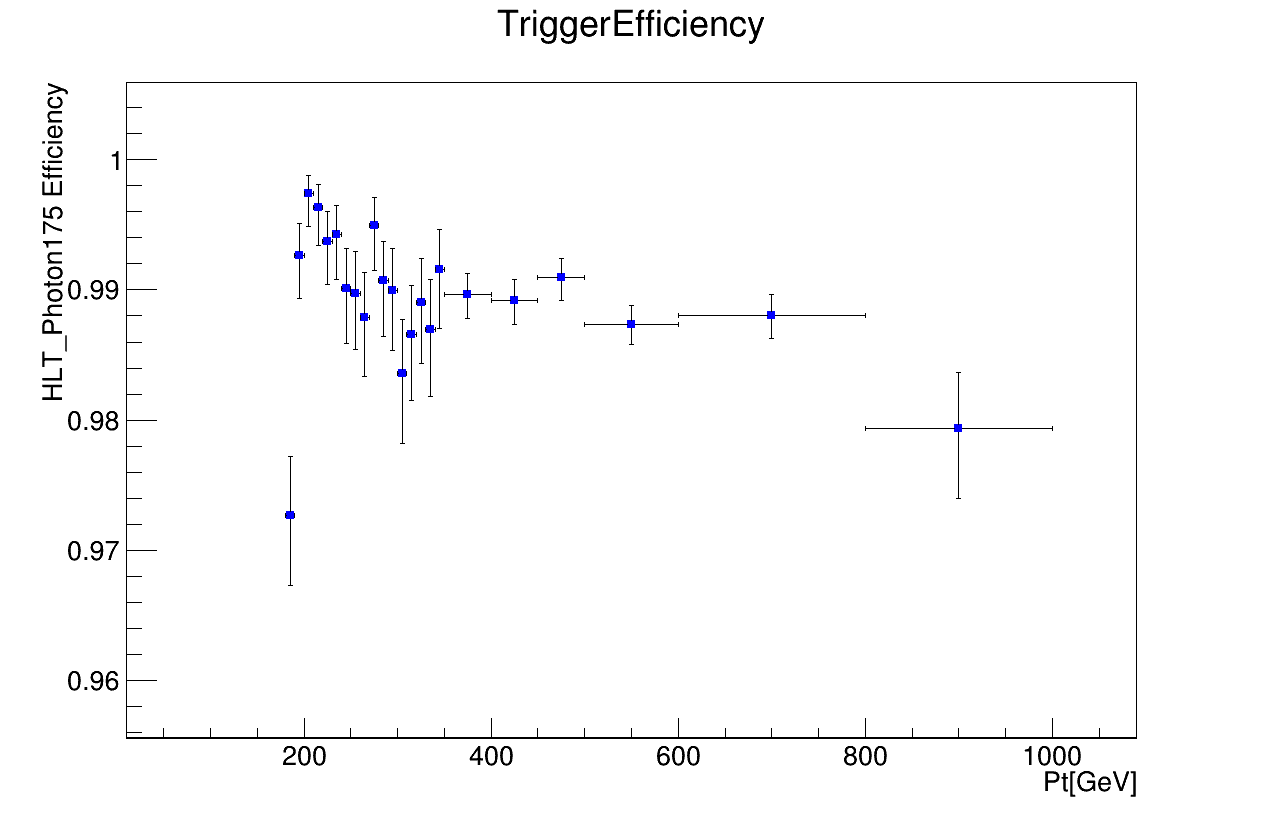
\includegraphics[width=0.75\textwidth]{Figures/triggereff_zoom.png}
    \caption{
    Absolute trigger efficiency of the monophoton HLT path HLT\_Photon165\_HE10.
    }
    \label{fig:trigger_efficiency}
  \end{center}
\end{figure}

In addition to passing the HLT path, every event must pass a set of \MET\ filters which guard against clearly spurious sources of \MET. If during some collision event
a detector element is not performing according to nominal specifications, e.g. because it is malfunctioning or turned off, the resulting reconstructed energy balance will
not be a reliable indicator of its true value. Events are rejected if they have a known instrumental issue of this sort.

\section{Photon} \label{sec:event_selection_photon}
Preliminary studies indicated that an \ETgamma\ cut of 175\unit{GeV} (along with a \MET\ cut of 170\unit{GeV}) would result in maximal discovery potential across
multiple BSM scenarios. Every event must contain at least one reconstructed photon with at least this much \ETgamma. Both here and below,
\ETgamma\ refers to the photon's raw supercluster \ET, for the reasons given in sec.~\ref{sec:reconstruction_egamma}. The photon candidate with the highest
\ETgamma\ is called the \textit{leading photon}.

Due to the high radiation fluences at high $|\eta|$, and the resulting use of VPTs instead of APDs, measurements of \ETgamma\ in the endcaps are significantly less precise
than those in the barrel. This reduces the statistical value of using EE photons, and we confirmed that their inclusion would not significantly alter the final results
of our analyses. Furthermore, the non-projective layout of EE crystals makes it much less straightforward to identify fake photons stemming from beam halo.
The leading photon must therefore lie within the barrel acceptance. To avoid energy leakage out of the barrel edges, as well as a layer of instrumentation partially
covering the outermost EB crystals, the leading photon must lie within $|\eta| < 1.4442$.

A photon originating from a neutral pion in a jet will tend to be accompanied by various other particles in a jet-sized $\Delta R$ cone. For a given type of PF particle
(photons, charged hadrons, or neutral hadrons), the corresponding \textit{isolation} (iso.) is defined to be the sum of particle energies for all particles of that type
within a $\Delta R < 0.3$ cone around the photon. A large iso.\ value indicates that the photon is likely to be fake.
In most CMS analyses, charged hadron iso.\ only considers charged hadrons with tracks linked to the leading PV. However,
the leading PV is chosen based on the sum of track $\pT^{2}$ of all tracks (and track \MET) linked to the PV, and monophoton vertices do not necessarily have charged tracks
with any substantial amount of \pT. The \textit{worst charged hadron iso.}, defined to be the maximum value of charged hadron iso.\ with respect to any vertex in the event,
gives a more robust estimate of charged hadron activity that is more suitable for monophoton events.

Calculation of a given type of iso.\ begins by summing the energies of all PF particles of that type near the photon. As pileup increases, an increasing number of PF particles
will be reconstructed out of pileup events, and so an increasing amount of iso.\ energy will reflect pileup energy. The energy carried by particles of a given type is observed to vary
linearly as a function of the estimated pileup energy density $\rho$. The slope of this linear dependence has dimensions of area and is called the \textit{effective area} ($A_{eff}$)
corresponding to particles of a given type. Subtracting $\rho{*}A_{eff}$ removes the pileup energy dependence from an iso.\ sum, leaving the \textit{corrected iso}.

The CMS monophoton group developed a custom monophoton ID for 2016 analyses, based on five variables: $H/E$, photon iso., worst charged iso., neutral iso., and the photon shower shape
variable \sieie\ defined by
\begin{equation}
\begin{gathered}
\begin{aligned}
\sieie &= \sqrt{\frac{\sum_{i\in5{\times}5} w_{i}(i\eta_{i} - {\bar{i\eta}}_{5{\times}5})^{2}}{\sum_{i\in5{\times}5} w_{i}}}\\
            w_{i} &= 4.7 + \ln{(E_{i} / E_{5{\times}5})}
\end{aligned}
\end{gathered}
\label{eq:sieie}
\end{equation}
where the sums run over the $5{\times}5$ crystal array centered on the supercluster seed, $E_{i}$ is the energy of crystal $i$, $E_{5{\times}5}$ is the sum of all crystal energies
in the $5{\times}5$ array, and (in the barrel) $i\eta_{i} - {\bar{i\eta}}_{5{\times}5}$ is the number of $\eta$-rows of separation between crystal $i$ and the center of the $5{\times}5$ array\footnote{The value
of 4.7 is essentially arbitrary. It scales \sieie\ so that a typical real photon in the barrel has $0.005 < \sieie < 0.011$.}. This variable
describes the energy spread of a photon's ECAL cluster---the more spread out a cluster is, the larger the value of \sieie.
The cuts defining the monophoton ID are listed in Table~\ref{tab:photonID}. The numerical values in these cuts were tuned to retain minimal jet fake events while retaining 80\% of
real \zinvg\ events in any $\ETgamma$ range above 175\unit{GeV}. Table~\ref{tab:effective_areas} lists the $A_{eff}$ values used to compute the corrected iso.

\begin{table}
\centering
\begin{tabular}{ c|c }
\hline
Variable & Cut value \\
\hline
$H/E$ & 0.0260 \\
\sieie & 0.01040 \\
corr.\ worst charged hadron iso.  & 1.146 \\
corr.\ neutral hadron iso. & $2.792 + 0.0112{*}\ETgamma + 0.000028{*}{\ETgamma}^{2}$ \\
corr.\ photon iso.  & $2.176 + 0.0043{*}\ETgamma$ \\
\hline
\end{tabular}
\caption{Cuts defining the 2016 monophoton ID, applicable to photons in the barrel.
A cut is passed if the expression in the left column is less than the value in the right column.
The effective areas used to compute the corrected iso.\ values are listed in Table~\ref{tab:effective_areas}.}
\label{tab:photonID}
\end{table}

\begin{table}
\centering
\begin{tabular}{ ccc }
\hline
Type of isolation & $|\eta| < 1.0$ & $1.0 < |\eta| < 1.479$ \\
\hline
worst charged hadron & 0.01064 & 0.1026 \\
neutral hadron & 0.0597 & 0.0807 \\
photon & 0.1210 & 0.1107 \\
\hline
\end{tabular}
\caption{Effective areas used in the 2016 monophoton ID.}
\label{tab:effective_areas}
\end{table}

The ID defined by the cuts in Table~\ref{tab:photonID} does not take into account whether or not the particle being ID'd has a corresponding track, relying instead solely on the distribution
of energy in the calorimeters in conjunction with the level of ``pollution'' of surrounding particles. The shower profiles of electrons are extremely similar to those of photons, and in principle
this ID works approximately as effectively to select real electrons, if track information is not taken into account. We obtain an estimate of the photon efficiency of this ID by examining its
efficiency for electrons, using the high cross-section $\PZ(\Pe\Pe)$ process as a ``standard candle'' for the \textit{tag-and-probe} method~\cite{ref:CMS-PAS-EGM-07-001}. An electron passing
tight ID requirements is identified as a tag electron, and a second electron passing much looser requirements is called the probe electron. The identity of the probe electron is reinforced by
its consistency with the $\PZ(\Pe\Pe)$ hypothesis: the event is selected as a good tag-and-probe event if the invariant mass of the tag--probe pair is close to the \PZ\ mass, and the background
of non-$\PZ(\Pe\Pe)$ events is estimated (and then subtracted out) by fitting an expected $\PZ(\Pe\Pe)$ shape along with an expected background shape to the invariant mass distribution.

In this case, the probe electron is examined to see if it passes the monophoton ID. The number of probes passing the ID, divided by the total number of probes examined, gives an estimate of the efficiency
of the monophoton ID. The photon ID efficiency was estimated using both observed and simulated data. The ratio of the two sets of efficiency measurements is shown in Fig.~\ref{fig:phoID_SF}.
Fitting a horizontal line to the figure, the ratio of the data efficiency to the MC efficiency is estimated to be $1.002 \pm 0.007$. This \textit{efficiency scale factor} is applied as an event
weight to all simulated events, and the uncertainty of 0.007 is propagated to the final analysis results through this weight.

\begin{figure}[hbtp]
  \begin{center}
    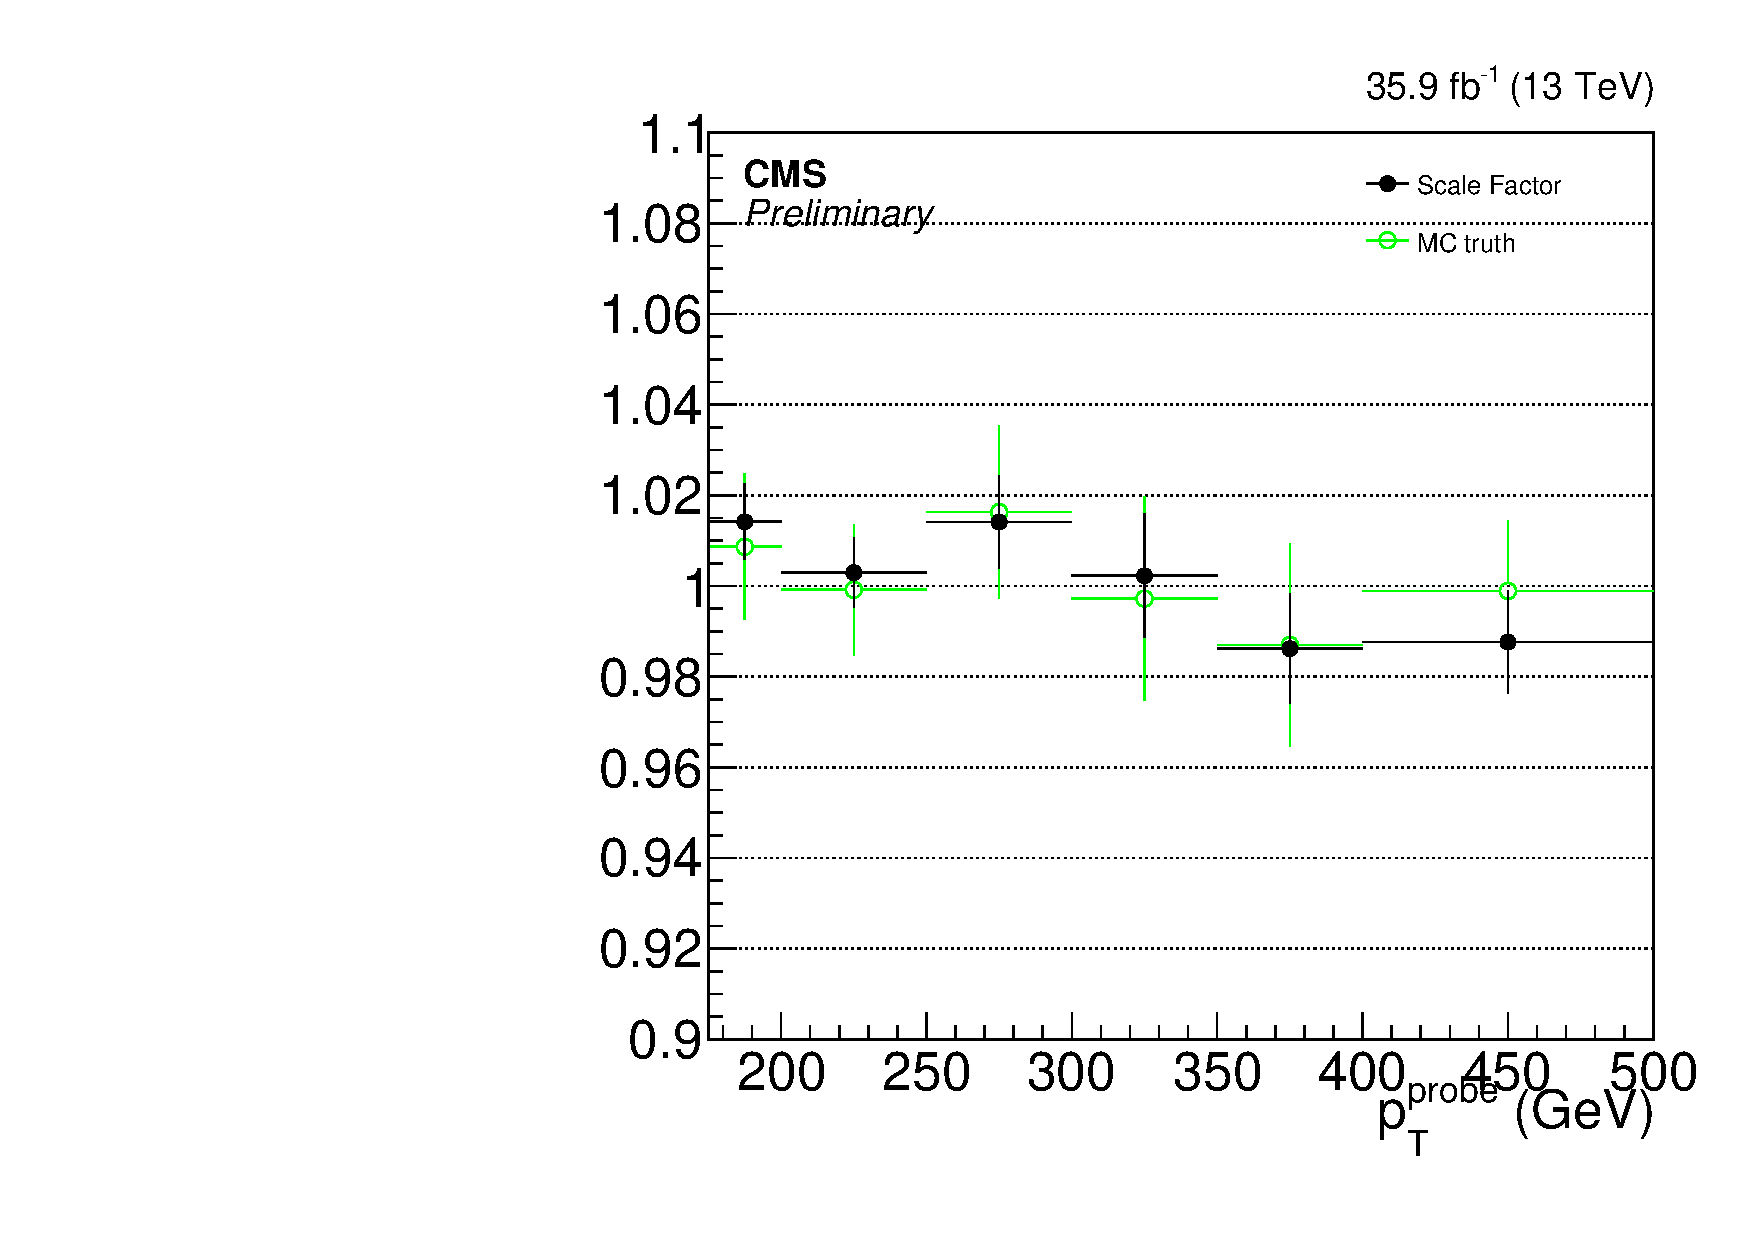
\includegraphics[width=0.65\textwidth]{Figures/phoID_SF.pdf}
    \caption{
    Efficiency scale factors for the monophoton ID requirements of Table~\ref{tab:photonID}, binned in terms of the probe electron \pT. The black points are obtained with the tag-and-probe method in
    both observed and simulated events. For the green points, the simulated efficiencies were instead calculated by geometrically matching the reconstructed electrons to generated electrons,
    and then dividing the number of matched electrons passing the ID by the total number of matched electrons. The two separate methods of computing the MC efficiency yield
    efficiency scale factors that are consistent within uncertainties in every \pT\ bin. The overall photon ID efficiency scale factor is obtained by fitting a horizontal line to this plot.
    }
    \label{fig:phoID_SF}
  \end{center}
\end{figure}

An electron may fake a photon if it has a well-reconstructed ECAL supercluster but a poorly-reconstructed track. A track may be reconstructed poorly if the electron failed to leave very many hits,
or if the hits it left were incorrectly assembled by the tracking algorithm. In these cases, the electron may still have left a \textit{pixel seed} consisting of at least two hits in the pixel tracker
with an inferred trajectory consistent with the supercluster~\cite{ref:1748-0221/10/08/P08010}. To remove as much of this background as possible, an event is only retained if the leading photon does
not have a matching pixel seed.

A real high-\pT\ photon essentially never has a \sieie\ value of 0.001 or less. Such a value is consistent with a single crystal having all or nearly all of the energy of the
reconstructed photon, which is much more consistent with a spike than with a real photon. The same applies to a \sipip\ value of 0.001 or less, where \sipip\ is
defined in a similar way as \sieie. In order to clean out spikes, an event is only retained if the leading photon has $\sieie > 0.001$ and $\sipip > 0.001$.

A beam halo muon impinging on EB will be traveling roughly parallel to the beamline, and can therefore leave energy deposits in a line of EB crystals extended in $\eta$ and narrow in $\phi$.
The sum of EB crystal energies in lines consistent with a beam halo muon, for any such lines passing through a given photon seed,
is the \textit{halo total energy} $E^\mathrm{halo}$. An event is only retained if $E^\mathrm{halo} < 4.9\unit{GeV}$.

Most hard \zinvg\ events occur within 3\unit{ns} of the nominal bunch collision time. In contrast, spikes tend to arrive more than 10\unit{ns} early, as described in sec.~\ref{sec:LHCCMS_CMS_ECAL}.
Beam halo accompanies the bunches and reaches the center of CMS just as the bunches collide. Photons from the bunch collision then take an additional few nanoseconds to reach ECAL,
with the net result being that beam halo tends to be reconstructed a few nanoseconds early. A photon arrival time cut of $|t| < 3\unit{ns}$ helps to further suppress these sources of background.

The efficiency of the preceding cuts (following the monophoton ID) is measured in a \gjets-enriched control region, defined by selecting events with at least one jet passing $\pT > 100\unit{GeV}$,
$|\eta| < 2.5$, and passing loose ID criteria. In addition, a $\MET < 60\unit{GeV}$ cut is applied to ensure that this control region is orthogonal to the signal regions. A photon
is selected which passes the monophoton ID cuts, with loosened worst charged iso.\ and \sieie\ requirements in order to be able to perform a template fit on the \sieie\ distribution.
This template fit is used to estimate and then subtract out the number of fake photons in this control region. A real photon template is taken from the \sieie\ distribution of real photons in
simulated \gjets\ events, and a fake photon template is taken from a high-worst-charged-iso. sideband. The templates are cleaned and systematic uncertainties are estimated using methods
very similar to those described in detail in sec.~\ref{sec:background_estimation_jetfake}.

A fit is performed on the observed distribution of all ID'd photons, and then a separate fit is performed on the observed distribution of
all ID'd photons that also pass the pixel seed, spike cleaning, and halo cleaning cuts. Each fit yields its own real photon count, and the ratio of those counts gives the observed efficiency
of the last set of cuts. The efficiency is estimated in simulation by counting the number of gen-matched reconstructed photons passing all cuts and
dividing by the number of photons passing at least the monophoton ID cuts. The ratio of the efficiency estimates in observed and simulated data, shown in Fig.~\ref{fig:pixseed_SF},
gives a second photon efficieny scale factor. Fitting a horizontal line to Fig.~\ref{fig:pixseed_SF} yields a value of $0.984 \pm 0.009$. This value is applied
as an event weight to all simulated data, and the corresponding uncertainty is propagated through this weight to the final results.

\begin{figure}[hbtp]
  \begin{center}
    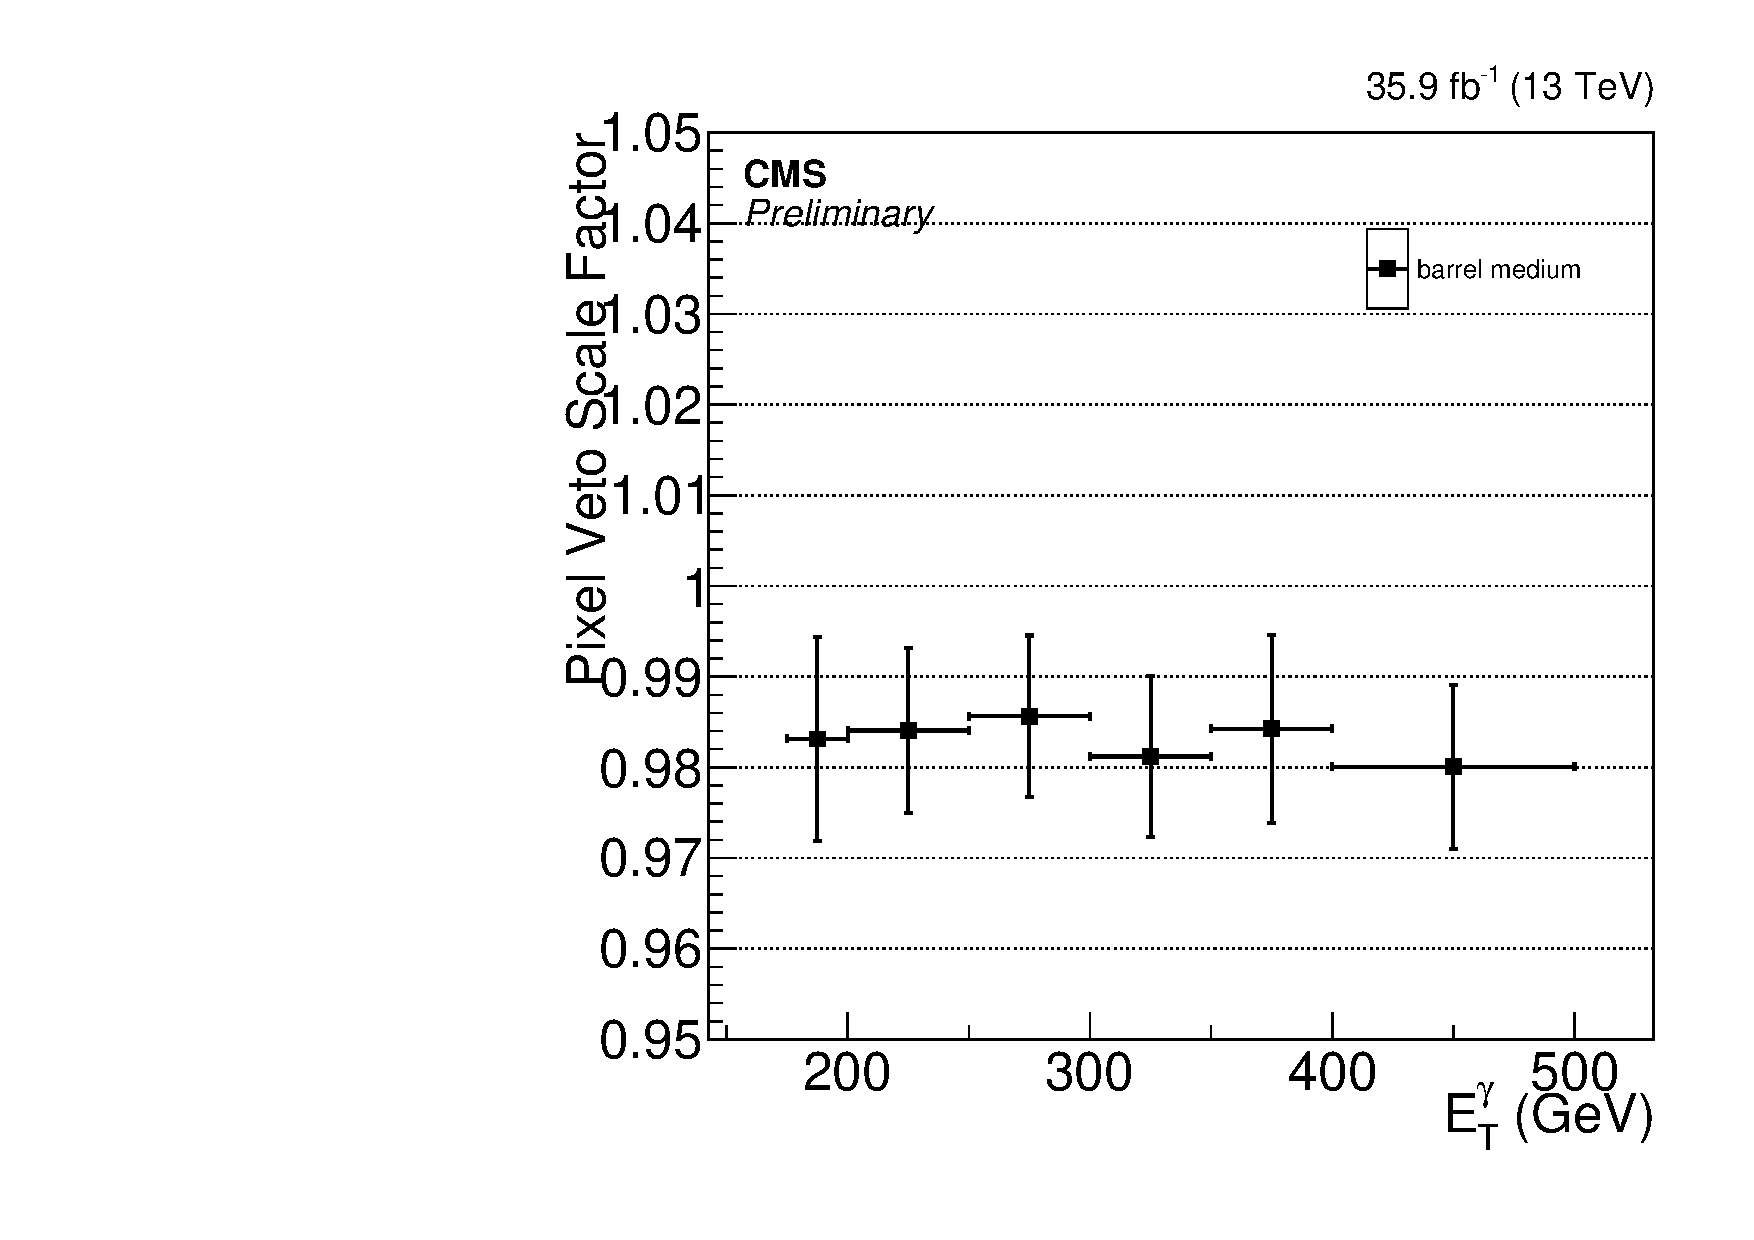
\includegraphics[width=0.65\textwidth]{Figures/pixseed_SF.pdf}
    \caption{
    Efficiency scale factors for the combined pixel seed, spike cleaning, and halo cleaning cuts.
    }
    \label{fig:pixseed_SF}
  \end{center}
\end{figure}

The variable $R_{9}$ is defined as the energy of the $3{\times}3$ crystal array centered on the most energetic crystal in the supercluster divided by the total supercluster energy.
A real, unconverted photon, very well-centered on one crystal, will tend to leave around 95\% of its energy in the $3{\times}3$ array; if the photon is converted, this fraction will
be smaller~\cite{ref:1748-0221/10/08/P08010}. The odds that a genuine high-\pT\ photon from a hard collision vertex will leave all of its energy in the $3{\times}3$ array
are close to zero. An $R_{9}$ value of 1.0 is more consistent with a spike, and so we only retain an event if the leading photon $R_{9}$ is strictly less than 1.0.

After these and all subsequent cuts are applied, a total of a few hundred observed events are left. On a first inspection of the data, we noted that O(10) selected events
were seeded from each of four single EB crystals. The vast majority of the 61\,200 EB crystals did not seed any events passing all cuts, and very few seeded more than one event.
We believe that these overproductive crystals were almost certainly producing entirely spurious photon candidates, as the result of a previously unidentified
instrumental malfunction, and we therefore reject any event in which the leading photon was seeded by one of these crystals.

As illustrated in Fig.~\ref{fig:beamhalo_sim}, beam halo muons are concentrated along the x-axis, which corresponds to values of $\phi$ close to either 0 or $\pi$ radians.
For the purpose of beam halo background estimation, the signal region is split into two parts based on $|\sin{\phi}|$ of the leading photon: $|\sin{\phi}| < \sin{0.5}$ defines
the horizontal signal region, and $|\sin{\phi}| > \sin{0.5}$ defines the vertical signal region. Much more beam halo is expected to fall in the horizontal than the vertical
signal region, in contrast to every other source of background, which is expected to be isotropic in $\phi$ and therefore fall into the two regions according to their
relative amount of angular coverage.

\section{Missing transverse momentum} \label{sec:event_selection_MET}
A pair of neutrinos recoiling against a photon with $\pTgamma > 175\unit{GeV}$ must have a correspondingly high \pT\ if no other high-\pT\ particles emerged
from the same \Pp\Pp\ collision, and must be traveling in a transverse direction opposite that of the photon. Each event in the signal regions must satisfy
$\MET > 170\unit{GeV}$, $\Delta\phi(\Pgamma,\vecMET) > 0.5\unit{rad}$, and $\ETgamma/\MET < 1.4$, ensuring that all selected events kinematically resemble a real \zinvg\ event.
In the control regions, the preceding \vecMET\ constraints are replaced by equivalent constraints on the \textit{recoil} \vecrecoil, defined to be the vector sum of \vecMET\ with
the \vecpT\ of the visible lepton(s) defining a given region.

To reject \gjets\ events in which the \MET\ is spuriously augmented by an under-measured jet \pT,
an event is only retained if the four leading jets in terms of \pT\ all satisfy $\Delta\phi(\mathrm{jet},\vecMET) > 0.5\unit{rad}$.
For the purpose of this cut, a ``jet'' is an AK4 CHS jet separated from the leading photon by $\Delta R > 0.4$, having $\pT > 30\unit{GeV}$ and
$|\eta| < 5.0$, and passing loose jet ID criteria. Since mismeasured jet \vecpT\ affects \vecMET\ directly, but not the \vecpT\ of any single
isolated lepton, this cut is applied without adjustment in the control regions (i.e.\ without replacing \vecMET\ by \vecrecoil).

\section{Lepton vetoes} \label{sec:event_selection_lepveto}
An event in the signal regions is rejected if either a veto electron or a veto muon is found. Leading and subleading leptons used
to select events for the control regions will fail this cut, and therefore the signal regions are completely separate from the control regions.
An event in one of the control regions is rejected if any additional veto electrons or muons are found beyond the leading and possibly subleading
leptons used to define the control region.

Veto electrons and muons must have $\pT > 10\unit{GeV}$, be separated from the leading photon by $\Delta R > 0.5$, lie within the tracking acceptance,
and pass a set of loose ID criteria. The ID criteria for veto electrons are listed in Table~\ref{tab:looseelectronID}.
A loose muon is a PF muon that is also either a tracker or global muon (or both).

\begin{table}
\centering
\begin{tabular}{ ccc }
\hline
Variable & $|\eta| < 1.479$ & $1.479 < |\eta| < 2.5$ \\
\hline
\sieie & 0.0103 & 0.0301 \\
$\Delta\eta(\mathrm{track\ at\ vertex}, \mathrm{supercluster\ seed})$ & 0.0105 & 0.00814 \\
$\Delta\phi(\mathrm{track\ at\ vertex}, \mathrm{supercluster})$ & 0.115 & 0.182 \\
$H/E$ & 0.104 & 0.0897 \\
sum of all iso.'s minus $\rho{*}A_{eff}$ & $0.0893{*}\pT$ & $0.121{*}\pT$ \\
$|1/E - 1/p|$ & 0.102 & 0.126 \\
$\Delta r(\mathrm{vertex}, \mathrm{origin})$ & 0.0261 & 0.118 \\
$\Delta z(\mathrm{vertex}, \mathrm{origin})$ & 0.41 & 0.822 \\
missing track hits & 3 & 2 \\
conversion vertices consistent with track & 1 & 1 \\
\hline
\end{tabular}
\caption{Loose ID cuts for electrons. The expression in the leftmost column must be strictly less than the value in either the middle or rightmost column, depending
on the electron's $|\eta|$. The effective areas used for electron ID's are listed in Table~\ref{tab:electron_effective_areas}.}
\label{tab:looseelectronID}
\end{table}

\begin{table}
\centering
\begin{tabular}{ cc }
\hline
$|\eta|$ range & $A_{eff}$ \\
\hline
$|\eta| < 1.0$ & 0.1752 \\
$1.0 < |\eta| < 1.479$ & 0.1862 \\
$1.479 < |\eta| < 2.0$ & 0.1411 \\
$2.0 < |\eta| < 2.2$ & 0.1534 \\
$2.2 < |\eta| < 2.3$ & 0.1903 \\
$2.3 < |\eta| < 2.4$ & 0.2243 \\
$2.4 < |\eta| < 2.5$ & 0.2687 \\
\hline
\end{tabular}
\caption{Effective areas for electron ID's.}
\label{tab:electron_effective_areas}
\end{table}

Events passing the photon, \MET, and lepton veto cuts described above are assigned to one of the two signal regions. Events that pass the photon
cuts as well as a set of control region cuts are assigned to the corresponding control region. The cuts defining each of the four control regions
are described in the next four sections. The various regions are defined so as to be mutually orthogonal, i.e.\ any one event can pass the cuts
for no more than one region.

\section{Single electron control region} \label{sec:event_selection_monoele}
The single electron control region is defined in essentially the same way as the signal regions, but requiring the presence of one (and only one) electron,
such that the electron and \vecMET\ are consistent with originating from a $\PW(\Pe\Pn)$ decay.
Instead of \vecMET, the photon \vecpT\ must be balanced by the recoil \vecrecoil, as discussed in sec.~\ref{sec:event_selection_MET}. The recoil in this
region is the vector sum of the leading electron \pT\ with \vecMET.
The leading SM process in the single electron control region is $\PW(\Pe\Pn)\Pgamma$ production; in contrast to the signal regions, \zinvg\ contributes
virtually nothing to this or to any of the other control regions.

Leading lepton ID criteria are relatively tight, in contrast to the loose ID requirements imposed on a veto or subleading lepton. A leading electron must have $\pT > 30\unit{GeV}$,
be separated from the leading photon by $\Delta R > 0.5$, and pass the set of cuts listed in Table~\ref{tab:tightelectronID}.
Consistency with $\PW(\Pe\Pn)$ decay is enforced by constraining the \textit{transverse mass} $m_\mathrm{T}$ of the electron--\MET\ system, defined by
\begin{equation}
m_\mathrm{T} = \sqrt{2*\pT^{\,\Pe}*\MET*(1 - \cos{\Delta\phi(\vecpT^{\,\Pe}, \vecMET)})}
\label{eq:mT}
\end{equation}
This must be less than 160\unit{GeV}, i.e.\ less than about twice the mass of the \PW. An additional $\MET > 50\unit{GeV}$ cut helps to further reduce background.

\begin{table}
\centering
\begin{tabular}{ ccc }
\hline
Variable & $|\eta| < 1.479$ & $1.479 < |\eta| < 2.5$ \\
\hline
\sieie & 0.0101 & 0.0279 \\
$\Delta\eta(\mathrm{track\ at\ vertex}, \mathrm{supercluster\ seed})$ & 0.00926 & 0.00724 \\
$\Delta\phi(\mathrm{track\ at\ vertex}, \mathrm{supercluster})$ & 0.0336 & 0.0918 \\
$H/E$ & 0.0597 & 0.0615 \\
sum of all iso.'s minus $\rho{*}A_{eff}$ & $0.0354{*}\pT$ & $0.0646{*}\pT$ \\
$|1/E - 1/p|$ & 0.012 & 0.00999 \\
$\Delta r(\mathrm{vertex}, \mathrm{origin})$ & 0.0111 & 0.0351 \\
$\Delta z(\mathrm{vertex}, \mathrm{origin})$ & 0.0466 & 0.417 \\
missing track hits & 3 & 2 \\
conversion vertices consistent with track & 1 & 1 \\
\hline
\end{tabular}
\caption{Tight ID cuts for electrons. The expression in the leftmost column must be strictly less than the value in either the middle or rightmost column, depending
on the electron's $|\eta|$. The effective areas used for electron ID's are listed in Table~\ref{tab:electron_effective_areas}.}
\label{tab:tightelectronID}
\end{table}

\section{Single muon control region} \label{sec:event_selection_monomu}
The single muon control region is, as the name implies, much like the single electron control region, but with a muon instead of an electron.
The recoil in this region is the vector sum of the leading muon \pT\ with \vecMET, and the leading SM process is $\PW(\Pmu\Pn)\Pgamma$ production.
A leading muon must have $\pT > 30\unit{GeV}$, be separated from the leading photon by $\Delta R > 0.5$, and pass the set of cuts listed in Table~\ref{tab:tightmuonID}.
Consistency with $\PW(\Pmu\Pn)$ decay is enforced by requiring that the muon--\MET\ $m_\mathrm{T}$ be no more than 160\unit{GeV}.

\begin{table}
\centering
\begin{tabular}{ cc }
\hline
Variable & Cut \\
\hline
corr.\ total iso. & $< 0.15{*}\pT$ \\
global muon & True \\
PF muon & True \\
track $\chi^{2}/\mathrm{NDF}$ & $< 10.0$ \\
muon chamber hits & $> 0$ \\
matched muon stations & $> 1$ \\
$\Delta r(\mathrm{vertex}, \mathrm{origin})$ & $< 0.2$ \\
$\Delta z(\mathrm{vertex}, \mathrm{origin})$ & $< 0.5$ \\
pixel tracker hits & $> 0$ \\
tracker layer hits & $> 5$ \\
\hline
\end{tabular}
\caption{Tight ID cuts for muons.}
\label{tab:tightmuonID}
\end{table}

\section{Dielectron control region} \label{sec:event_selection_diele}
In the dielectron control region, a subleading electron must be selected in addition to the leading electron, such that the two electrons
are consistent with originating from a $\PZ(\Pe\Pe)$ decay.
The recoil in this region is the vector sum of the leading electron \pT, subleading electron \pT, and \vecMET, and the leading SM process
is $\PZ(\Pe\Pe)\Pgamma$ production. A leading electron must pass the tight ID criteria listed in Table~\ref{tab:tightelectronID},
and a subleading electron must pass the loose ID criteria in Table~\ref{tab:looseelectronID}.
Consistency with $\PZ(\Pe\Pe)$ decay is enforced by requiring that the leading and subleading electrons have opposite charges, and that the invariant mass of the
electron pair lies between 60 and 120\unit{GeV}, i.e.\ within about 30\unit{GeV} of the \PZ\ mass.

\section{Dimuon control region} \label{sec:event_selection_dimu}
Finally, the dimuon control region is much like the dielectron control region, but with muons instead of electrons.
The recoil in this region is the vector sum of the leading muon \pT, subleading muon \pT, and \vecMET, and the leading SM process
is $\PZ(\Pmu\Pmu)\Pgamma$ production. A subleading muon must pass the loose muon ID criteria listed in sec.~\ref{sec:event_selection_lepveto}.
Consistency with $\PZ(\Pmu\Pmu)$ decay is enforced by requiring that the leading and subleading muons have opposite charges, and that the invariant mass of the
muon pair lies between 60 and 120\unit{GeV}.

\chapter{Signal and background estimation} \label{chap:background_estimation}
\section{Yields from simulation} \label{sec:background_estimation_simulated}
If a well-validated MC sample exists for a given process (Ch.~\ref{chap:simulation}), and if appropriate data--MC correction factors are applied (Ch.~\ref{chap:event_selection}),
the expected event yield contributed by that process to a given signal or control region may be estimated entirely within simulation.
After generating some large number of events (sufficient to render statistical uncertainties negligible with respect to other sources of uncertainty),
running them through the detector simulation, and reconstructing the results, the appropriate signal or control region cuts are finally applied to the simulated events.
The number of events passing all cuts, divided by the total number of events generated, gives a maximum-likelihood (ML) estimate of the probability that
an event of the kind modeled by the sample will contribute to the final observed event tally. This probability is often written as the product of two factors: the
probability that an event lies within the kinematic coverage of the detector, and the probability that an event within the kinematic coverage passes selection cuts,
called the \textit{acceptance} ($A$) and \textit{efficiency} ($\epsilon$), respectively. The expected contribution of a given process to a final event tally is therefore given by
\begin{equation}
\mathrm{expected\ yield} = A*\epsilon*\sigma*L
\end{equation}
where $\sigma$ is the total cross section of a given process (having kinematic properties within the range modeled by the MC sample) and $L$ is the integrated
luminosity of the observed dataset (35.9\fbinv).

\section{Electron faking photon} \label{sec:background_estimation_elefake}
An inclusive estimate of the electron faking photon yield, summed over all processes with an isolated final-state electron, is obtained using a \textit{fake ratio} method.
The ratio of the numbers of successful vs. unsuccessful fakes is evaluated in a dedicated control region, designed in such a way that this ratio is expected to be equally
valid in the signal regions. Multiplying this ratio by the observed number of unsuccessful fake events in the signal regions gives an estimate of the number of successful
fake events in the signal regions. This last step in particular distinguishes the fake ratio method from e.g. finding a data--MC correction factor and applying that to
a purely MC-derived estimate of electron fake yields. Since the final expected yield is proportional to a set of observed (as opposed to simulated) data,
this is known as a \textit{data-driven} method.

An electron fakes a photon if it is misreconstructed as a PF photon and passes the photon ID cuts, including the pixel seed veto. This last cut is key because electrons
and photons have substantially similar ECAL shower profiles, and are primarily distinguished by the presence or absence of a charged track.
The fake ratio is estimated using a tag-and-probe method in a $\PZ{\rightarrow}\Pe\Pe$ control region, in which the tag is
a reconstructed electron that passes tight electron ID cuts, and the probe is a reconstructed photon that passes all photon ID cuts (ignoring the pixel
seed veto)\footnote{All control regions defined in this chapter also require the monophoton HLT path as well as the \MET\ filters to be passed.}.
In this case the probe is confirmed to be an electron by the event's compatibility with the $\PZ{\rightarrow}\Pe\Pe$ hypothesis, which is ensured by requiring that the invariant mass
of the electron-photon pair is close to the $Z$ mass.

Some processes other than $\PZ{\rightarrow}\Pe\Pe$ can nevertheless fake this signature, and the number of such background events is estimated using a template fitting method,
in which the template shapes are analytic functions of the \Pe\Pe\ invariant mass.
The $\PZ{\rightarrow}\Pe\Pe$ template is a Breit-Wigner distribution convoluted with the Crystal Ball function.
The background template is a sigmoid function convoluted with an exponential function.
The mass and width parameters of the Breit-Wigner distribution are fixed to the mass and width of the \PZ\ as reported by PDG, while the parameters of the other functions
are allowed to vary freely in the fit.

Separate template fits are performed in four different bins of reconstructed \ETgamma.
The fits are further separated by whether the probe has a matching pixel seed. These are illustrated in Fig.~\ref{fig:efake_fits}.
After the fits, the integrals of the signal templates with and without
pixel seeds in reco bin $j$ are denoted by $N^{\Pe\Pe}[j]$ and $N^{\Pe\gamma}[j]$, respectively.
The fake ratio $R_{\Pe}[j]$ in reco bin $j$ is estimated to be $N^{\Pe\gamma}[j] / N^{\Pe\Pe}[j]$.

\begin{figure}[htbp]
  \begin{center}
    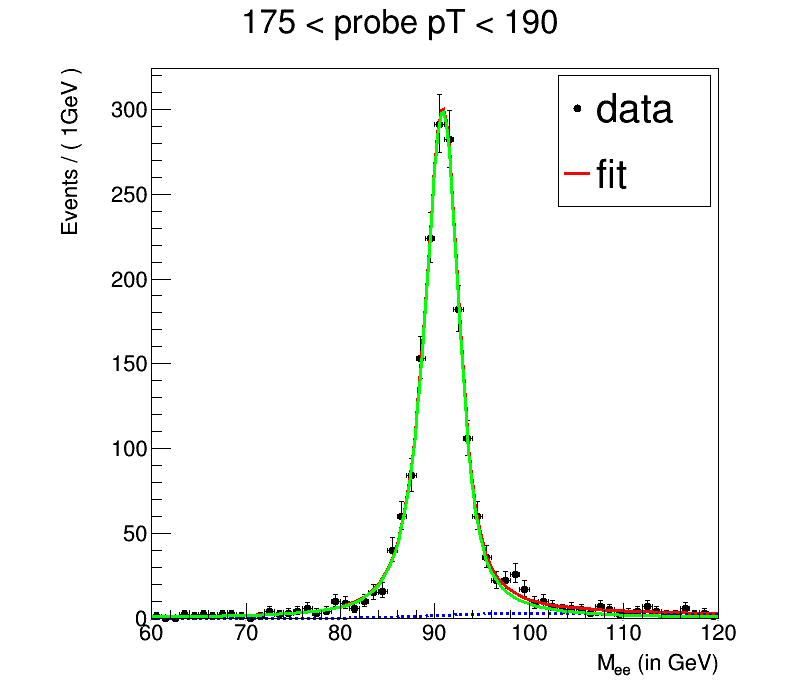
\includegraphics[width=0.40\linewidth]{Figures/efake/EE175190.png}
    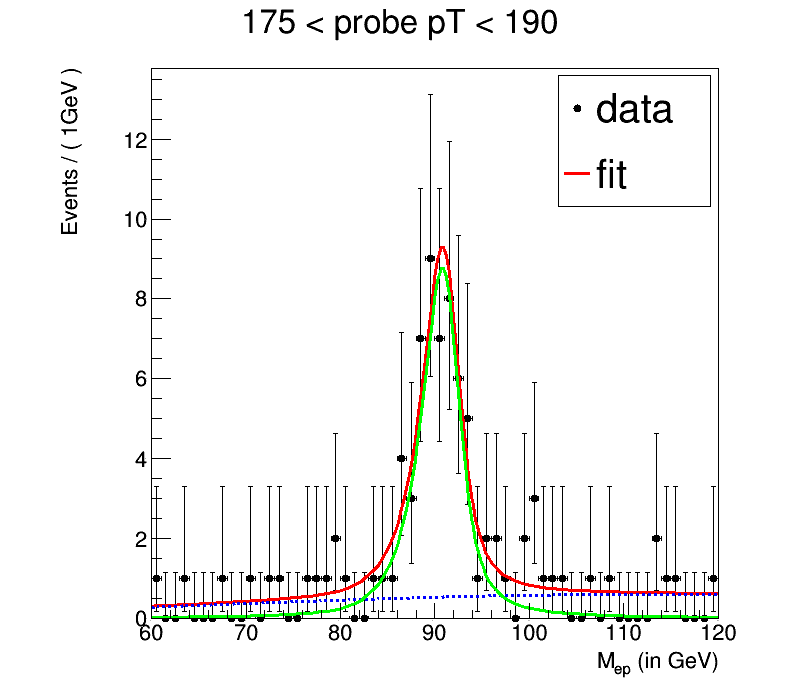
\includegraphics[width=0.40\linewidth]{Figures/efake/EP175190.png}
    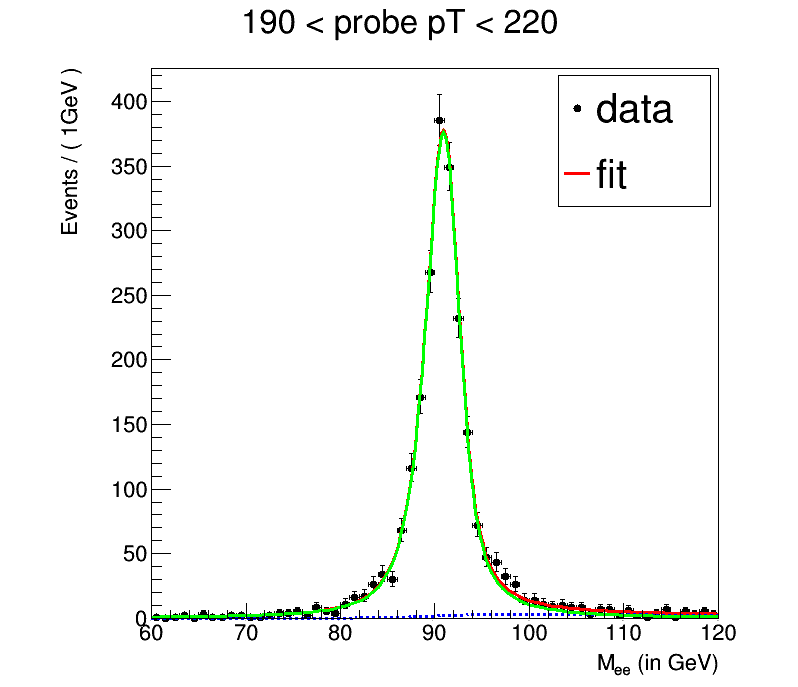
\includegraphics[width=0.40\linewidth]{Figures/efake/EE190220.png}
    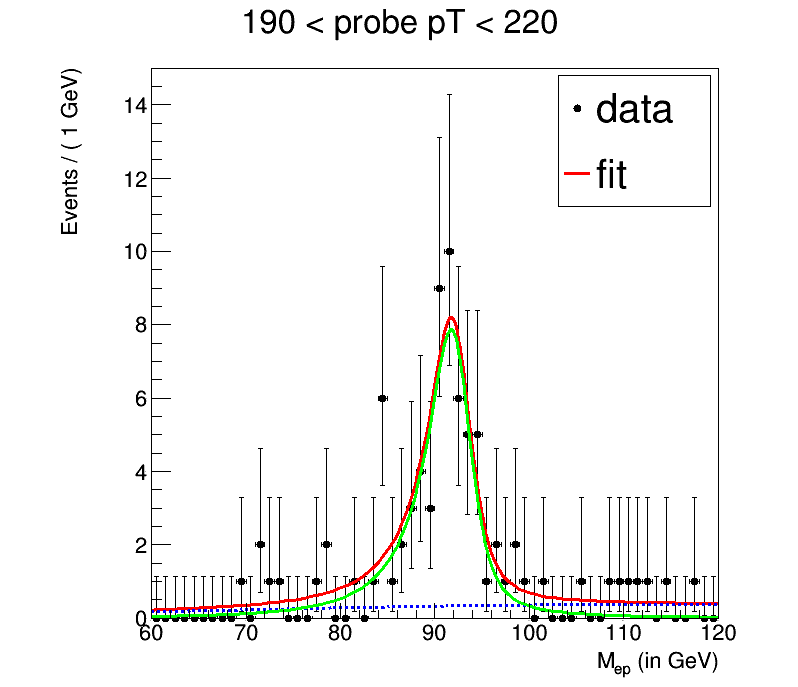
\includegraphics[width=0.40\linewidth]{Figures/efake/EP190220.png}
    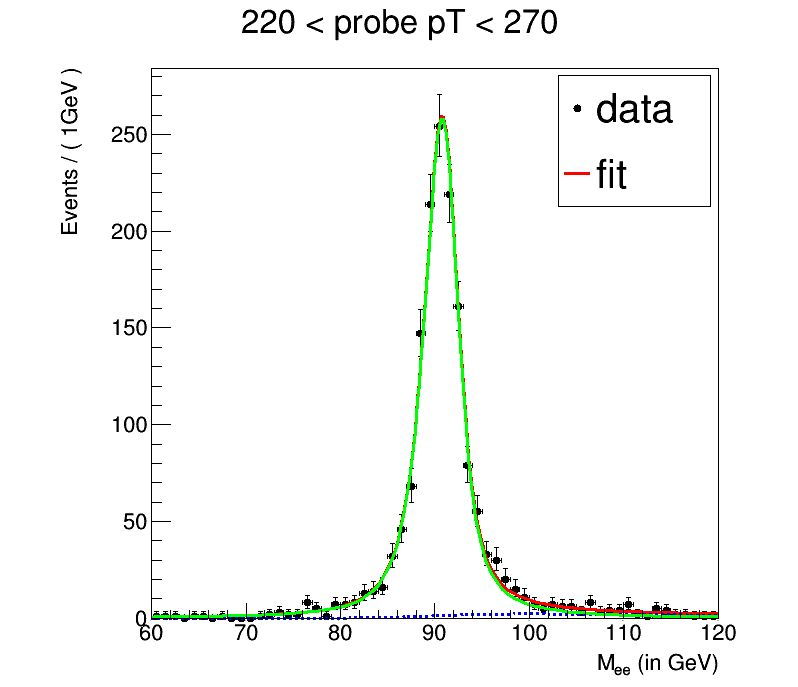
\includegraphics[width=0.40\linewidth]{Figures/efake/EE220270.png}
    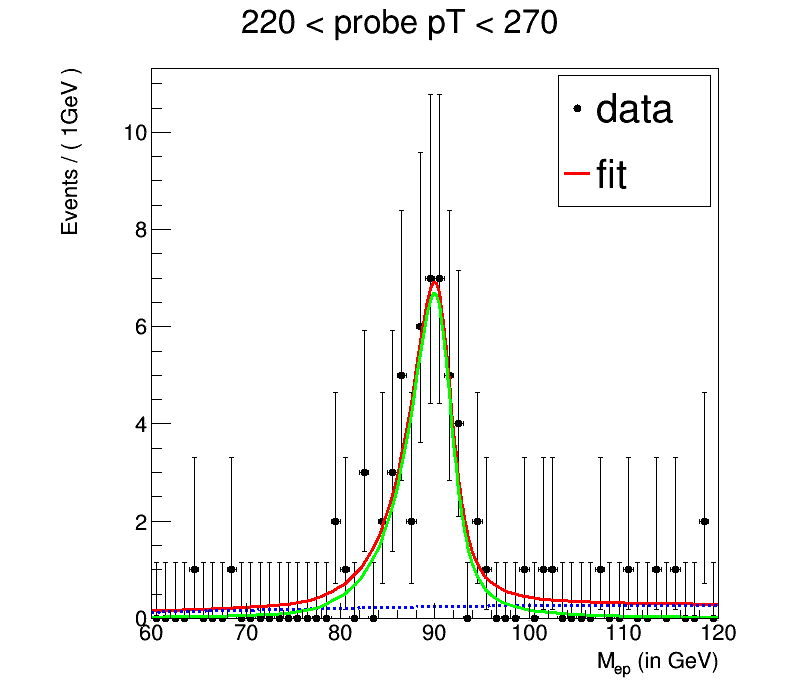
\includegraphics[width=0.40\linewidth]{Figures/efake/EP220270.png}
    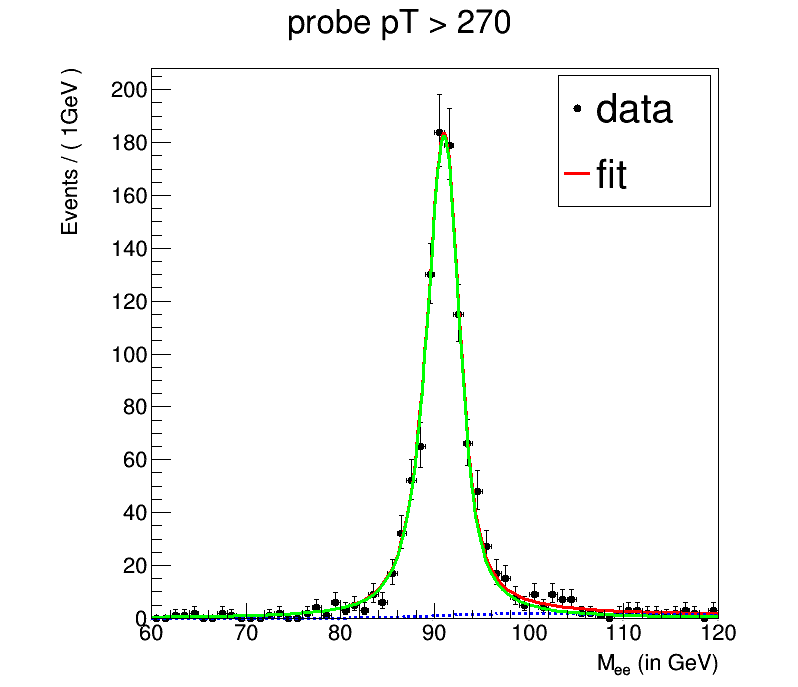
\includegraphics[width=0.40\linewidth]{Figures/efake/EE270.png}
    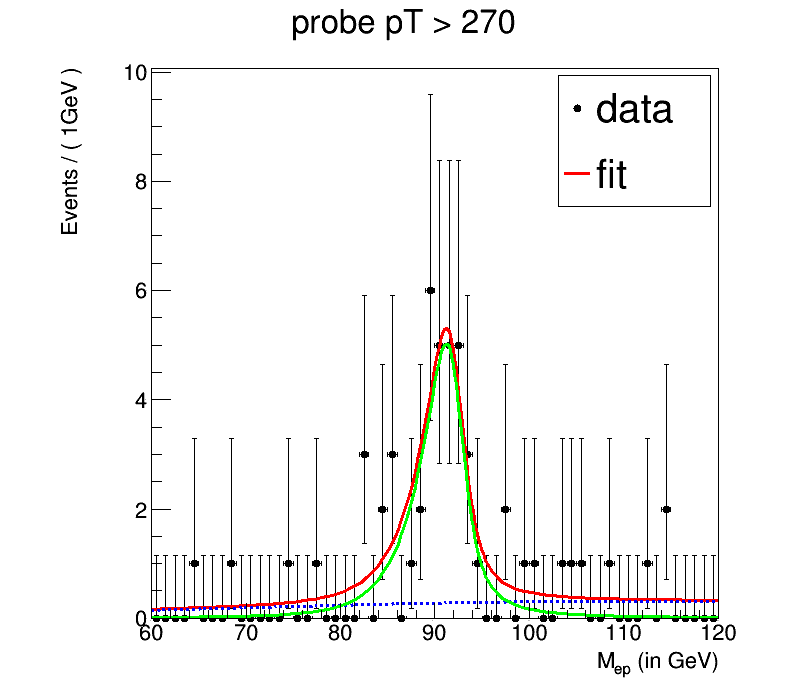
\includegraphics[width=0.40\linewidth]{Figures/efake/EP270.png}
    \caption{
      Fits to the mass distributions for $\Pe\Pe$ (left) and $\Pe\gamma$ (right) selections, in bins of probe \pT: $175 < \pT < 190\unit{GeV}$ , $190 < \pT < 220\unit{GeV}$ , $220 < \pT > 270\unit{GeV}$  and $ \pT > 270\unit{GeV}$.
      The blue dashed curve is the background template, and the red solid curve is the sum of the signal and background templates.
    }
    \label{fig:efake_fits}
  \end{center}
\end{figure}

To estimate the statistical uncertainty on $R_{\Pe}[j]$, 100 samples of random ``toy'' $\PZ{\rightarrow}\Pe\Pe$ events are generated using
the signal template as the underlying distribution. The samples each have the same number of events as the original data sample.
For each sample, the fit is redone using the toy mass distribution as the ``observed'' distribution. The
statistical uncertainty on $R_{\Pe}[j]$ is then taken to be the standard deviation of the toy $R_{\Pe}[j]$ estimates.
The systematic uncertainties on $R_{\Pe}[j]$ are estimated by redoing the fits with alternative signal and background templates.
The alternative signal template is taken from a $\PZ{\rightarrow}\Pe\Pe$ MC sample, and the alternative background template is a second
order polynomial function. The systematic uncertainty from each type of variation is taken to be the shift in the fit result following the variation.
This source of uncertainty is dominated by the signal template uncertainty.

The values of $R_{\Pe}[j]$, along with their uncertainties, are shown in Table~\ref{tab:efake}.
The fake ratio does not appear to vary significantly with \ETgamma.
Under the assumption that the fake ratio is essentially constant, a flat line is fit to $R_{\Pe}[j]$ as a function of \ETgamma. The resulting
y-intercept of 0.03031 is taken to be the constant value of $R_{\Pe}$ for all \ETgamma, with a combined uncertainty of 0.00220.
To estimate the number of events where electrons fake photons in all respects, events are first selected with reconstructed photons
that pass all the photon ID cuts, except that they have matching pixel seeds, and the number of such events is multiplied by
by $R_{\Pe}$.

\begin{table}
  \begin{center}
    \caption{$R_{\Pe}$ and its relative statistical and systematic uncertainties, as a function of probe \pT.}
    \label{tab:efake}
    \begin{tabular}{| c | c | c | c|}
      \hline
      Probe \pT\ [GeV] & $R_{\Pe}$ & Statistical (\%)  & Systematic (\%)  \\
      \hline
      \hline
      $[175, 190]$ &  0.032 & 12.3 & 4.4 \\
      \hline
      $[190, 220]$ & 0.027 & 11.1 & 8.2 \\
      \hline
      $[220, 270]$ &  0.031 & 12.2 & 3.6 \\
      \hline
      $[270, inf]$ &  0.034 & 14.9 & 12.6 \\
      \hline
    \end{tabular}
  \end{center}
\end{table}

\section{Jet faking photon} \label{sec:background_estimation_jetfake}
Like the electron faking photon background, the expected jet faking photon background is estimated via a data-driven method employing a fake ratio.
The numerator of the fake ratio should be the number of fake photon events originating from jets (passing any given signal or control region definition), and so
is defined by selecting events with a leading photon passing our standard photon ID.
The denominator should the number of events in which a high-\ET\ reconstructed photon is surrounded by so much energy from other particles
that it fails a loose set of isolation criteria (and so the photon is likely a jet constituent rather than a true hard-process photon); it is defined by selecting events
with a photon failing a relatively loose ID that has a 90\% selection efficiency for real photons\footnote{Denominator events must still pass a
``very loose'' ID with five times higher maximum isolation cuts.}.

The fake ratio is esimated by counting the number of numerator and denominator events in a control region defined by $\MET < 30\unit{GeV}$. Both the observed
numerator and denominator yields are expected to receive ``contamination'' from real hard-process photon events. The expected contribution of real hard-process
photons to the observed numerator yield is estimated (and subtracted out) by fitting real and fake photon templates to the photon \sieie\ distribution of numerator
events. The real photon template is estimated using \gjets\ MC. The fake photon template is derived from observed event yields in a \textit{sideband} region in which
the leading photon has worst charged hadron isolation lying between 8 and 14\unit{GeV}, but otherwise passes numerator cuts.
This sideband was chosen for the relative absence of real photon contamination. Nevertheless, some residual real photon events are still expected to contribute, and
the fake template is finally ``cleaned'' by subtracting the expected \sieie\ distribution of real photon events estimated in \gjets\ MC.

\begin{figure}[hbtp]
  \begin{center}
  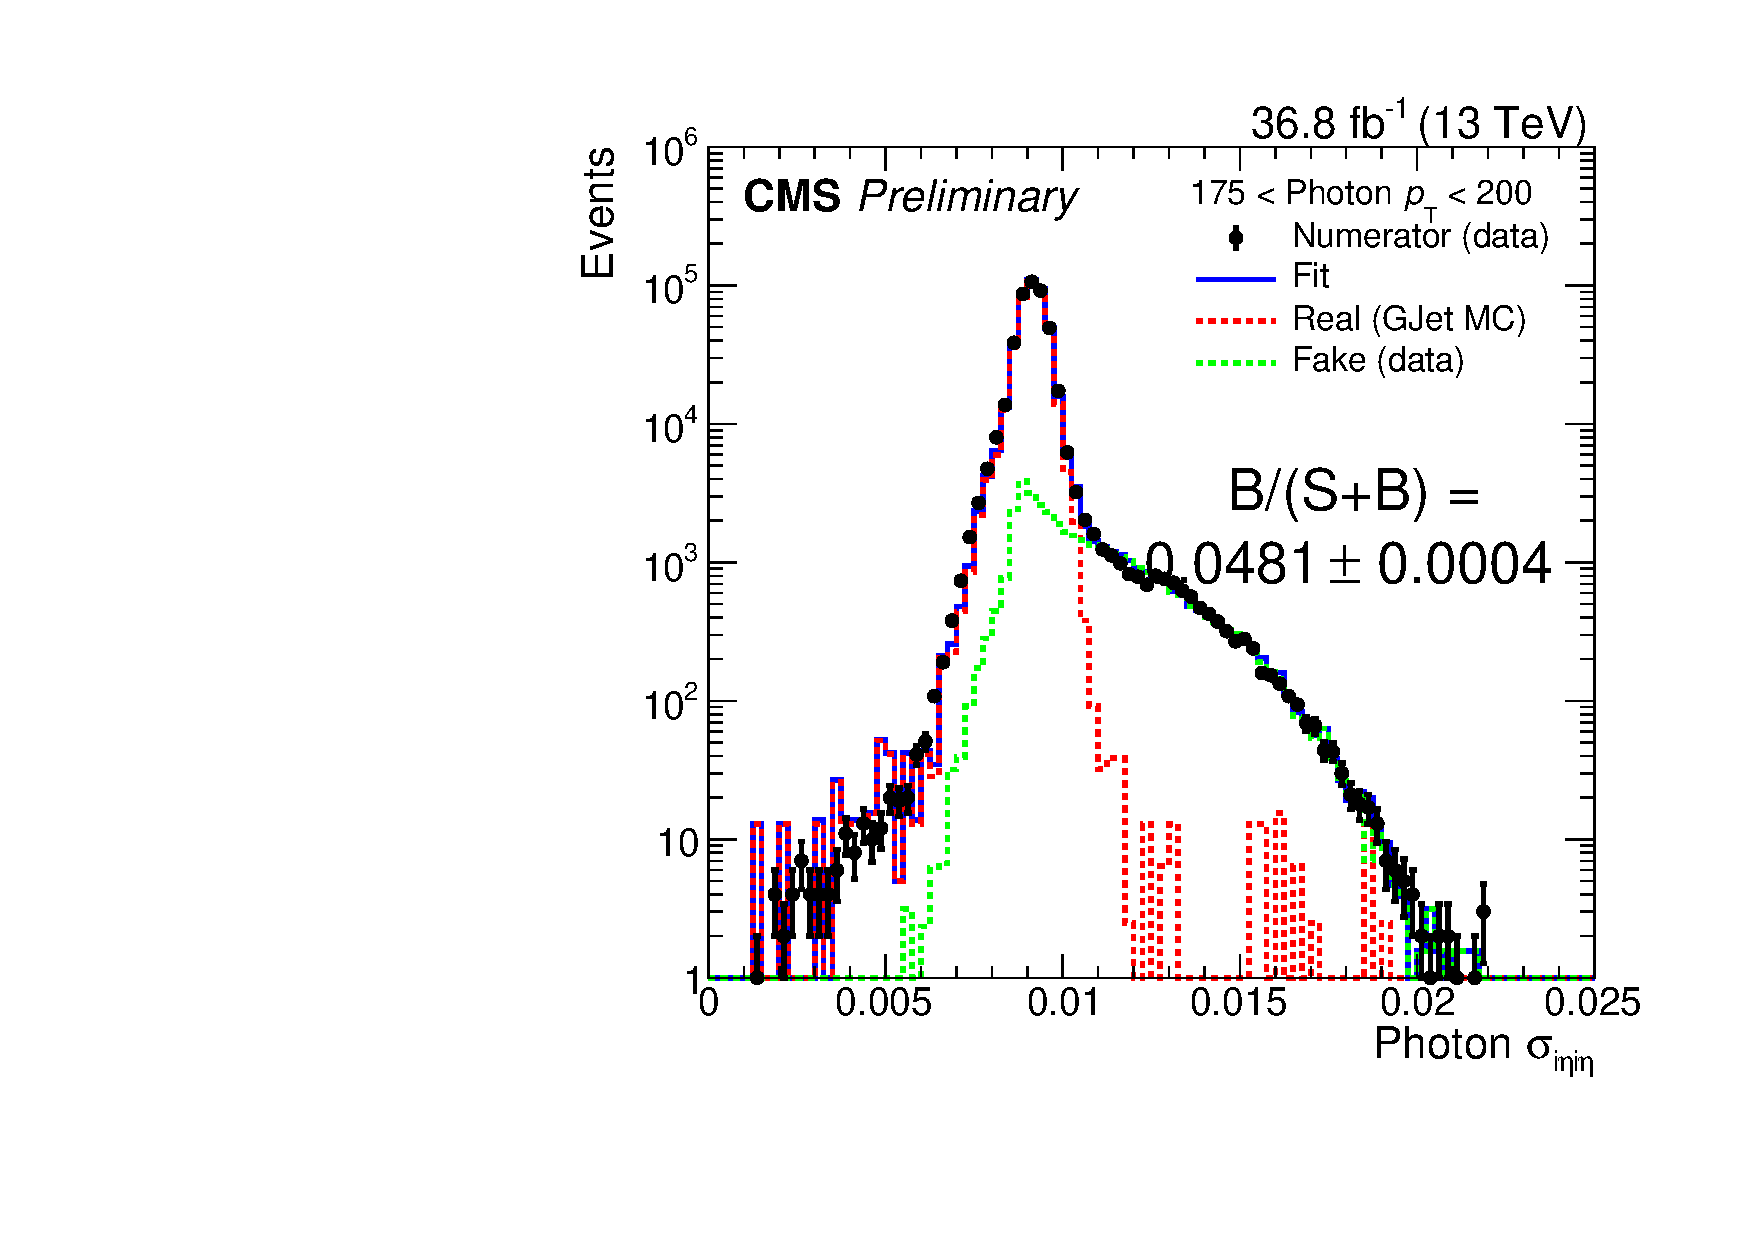
\includegraphics[width=0.45\textwidth]{Figures/QCD/num_fit_175to200.pdf}
  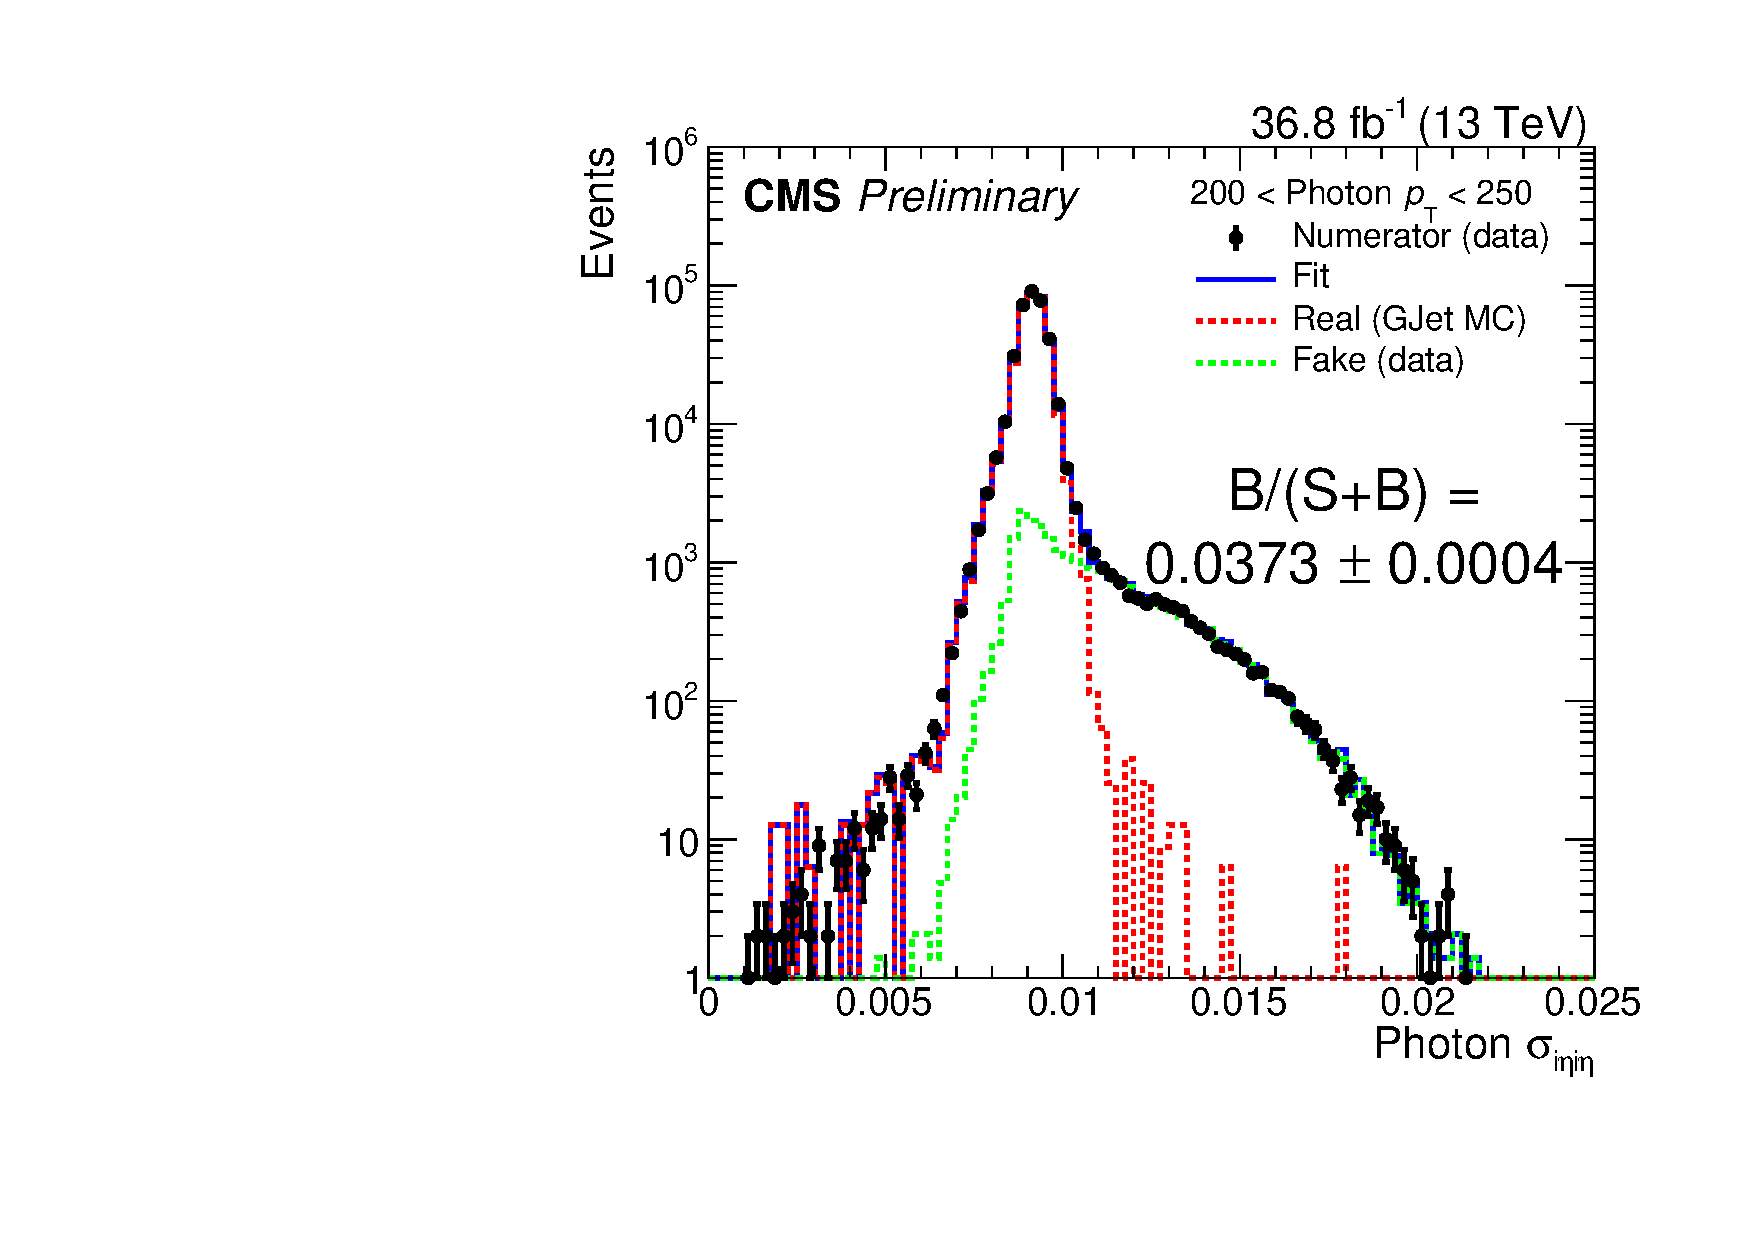
\includegraphics[width=0.45\textwidth]{Figures/QCD/num_fit_200to250.pdf}
  \caption{Distributions of photon $\sigma_{i\eta i\eta}$ in data, and fits to real and fake photon components, in \ETgamma\ bins 175-200\unit{GeV} and 200-250\unit{GeV}.
  The template fitting is done over the whole \sieie\ distribution seen here, and then the fake ratio numerator is computed by integrating the fake photon template (green)
  from 0 to 0.0104, corresponding to the monophoton ID cut. B/(S+B) refers to the fraction of fake events compared to all observed numerator events within this region of integration.}
  \label{fig:qcd_fits_a}
  \end{center}
\end{figure}

\begin{figure}[hbtp]
  \begin{center}
  \includegraphics[width=0.45\textwidth]{Figures/QCD/num_fit_250to300.pdf}
  \includegraphics[width=0.45\textwidth]{Figures/QCD/num_fit_300to400.pdf}
  \caption{Distributions of photon $\sigma_{i\eta i\eta}$ in data, and fits to real and fake photon components, in \ETgamma\ bins 250-300\unit{GeV} and 300-400\unit{GeV}.
  The template fitting is done over the whole \sieie\ distribution seen here, and then the fake ratio numerator is computed by integrating the fake photon template (green)
  from 0 to 0.0104, corresponding to the monophoton ID cut. B/(S+B) refers to the fraction of fake events compared to all observed numerator events within this region of integration.}
  \label{fig:qcd_fits_b}
  \end{center}
\end{figure}

\begin{figure}[hbtp]
  \begin{center}
  \includegraphics[width=0.45\textwidth]{Figures/QCD/num_fit_400to1000.pdf}
  \caption{Distributions of photon $\sigma_{i\eta i\eta}$ in data, and fits to real and fake photon components, in \ETgamma\ bin 400-1000\unit{GeV}.
  The template fitting is done over the whole \sieie\ distribution seen here, and then the fake ratio numerator is computed by integrating the fake photon template (green)
  from 0 to 0.0104, corresponding to the monophoton ID cut. B/(S+B) refers to the fraction of fake events compared to all observed numerator events within this region of integration.}
  \label{fig:qcd_fits_c}
  \end{center}
\end{figure}

The above procedure ensures a robust estimate of the fake photon yield in the numerator within the $\MET < 30\unit{GeV}$ control region.
The fake photon yield must also be estimated in the denominator, with the
additional constraint that it must be estimated in the same way both in the $\MET < 30\unit{GeV}$ control region and in any other signal or control regions in which
the final jet faking photon yield is needed. In such other regions, the template fitting method described above is not practicable. Instead, an additional
cut is applied on photon \sieie\ in the denominator to remove any possible real photons, so as to preserve a consistent denominator composition in any control region.
Inverting the \sieie\ cut from the monophoton ID ensures that nearly 100\% of real photon events (as estimated in \gjets\ MC) are removed from the denominator,
while preserving a maximal number of fake photon events.

Both the numerator template fitting and studies of denominator purity depend on having reliable MC estimates of the \sieie\ distribution of real photon events.
Studying the \sieie\ distributions of electrons in tag-and-probe samples in both MC and data reveals a consistent discrepancy between the two, of up to a few percent.
Electrons and photons have very similar \sieie\ distributions, and the data vs. MC discrepancy is believed to be similar
for both types of particles. To correct this discrepancy, the photon \sieie\ shapes obtained in MC are multiplied by the ratio of the electron \sieie\ shape from data
over the corresponding electron \sieie\ shape from MC.

The resulting fake ratio is illustrated in Fig.~\ref{fig:qcd_fake_ratio}.
It is assumed to have approximately the same value regardless of which signal or control region cuts are applied. However, the $\MET < 30\unit{GeV}$ cut
that defines the fake ratio control region is substantially different from the $\MET > 170\unit{GeV}$ cut defining the signal regions, and jets
are complex multiparticle objects that are relatively likely to have mismeasured $\MET$.
To study the possible impact of shifting \MET\ cut definitions on the fake ratio,
the ratio is reevaluated for control regions defined by $\MET < (7/6)\times30\unit{GeV}$ and $\MET < (5/6)\times30\unit{GeV}$.
Other variations in the fake ratio are obtained by shifting the maximum allowed charged hadron isolation in the sideband region up and down by 2\unit{GeV};
shifting the \sieie\ corrections up and down by their uncertainties; and using finer or coarser histogram binning in the numerator templates. Statistical
uncertainties due to limited data and uncertainties stemming from the template fitting procedure are also propagated to the fake ratio. The total uncertainty
on the fake ratio is taken to be the size of the envelope of all of the separate shifts. These shifts are illustrated in Fig.~\ref{fig:qcd_fake_ratio}.

\begin{figure}[hbtp]
  \begin{center}
  \includegraphics[width=0.45\textwidth]{Figures/QCD/QCDfake_fakeratio.pdf}
  \includegraphics[width=0.45\textwidth]{Figures/QCD/QCDfake_systematics.pdf}
  \caption{The jet fake ratio as a function of \ETgamma\ (left), and fractional variations in that ratio caused by shifts of various types (right).}
  \label{fig:qcd_fake_ratio}
  \end{center}
\end{figure}

\section{Spikes} \label{sec:background_estimation_spikes}
Due to their idiosyncratic means of production, spikes do not currently have simulated samples that could be expected to accurately reproduce their expected yield,
particularly in the case of events somehow passing all the spike cleaning cuts in the monophoton signal regions. Instead, the time distribution of clearly-identified
spikes in observed events can be used to extrapolate the preponderance of spikes within the in-time window ($|t|<3\unit{ns}$) defined by our signal region cuts.
This time distribution is examined by performing a custom reconstruction of the data in which ``spike-killer'' cuts that are part of standard event reconstruction
are omitted. Spike candidates are selected from reconstructed photons that pass a loosened set of ID criteria with no isolation cuts (to account for the different
characteristics of events outside the in-time window) but have $\ETgamma > 175\unit{GeV}$, $\sieie < 0.0104$, and either \sieie\ or $\sipip < 0.1$.
As illustrated in Fig.~\ref{fig:fulltime_templates}, this distribution exhibits a peak around $t = -15\unit{ns}$ and falls off to near zero by the in-time window.

The time distribution of spike candidates is one of three templates used to fit the timing distribution of monophoton-like events from $t = -25\unit{ns}$ to $+25\unit{ns}$,
where a ``monophoton-like event'' is defined to be an event with $\MET > 170\unit{GeV}$ and a reconstructed photon with $\ETgamma > 175\unit{GeV}$ and $0.001 < \sieie < 0.0104$.
candidate events are chosen based on reconstructed photons with MIP total energy greater than 4.9\unit{GeV}. Electron candidate events are chosen based on a
$\PZ{\rightarrow}\Pe\Pe$ tag-and-probe selection similar to that used for the electron fake ratio, in which the probe is a reconstructed photon that has a pixel
seed and serves as the particle whose time is templated. Electron candidates reconstructed as photons have a timing distribution essentially identical to real
photons, with the added advantage that other information in the event (such as the pixel seed) marks these as originating directly from the hard collision process.
The three templates and their fit to the full time distribution are shown in Figs.~\ref{fig:fulltime_templates} and \ref{fig:fulltime}.

\begin{figure}
  \begin{center}
    \includegraphics[width=8.0cm,height=6.5cm]{Figures/noncol/TemplatesQuadZ.pdf}
    \caption{
      Time distribution templates for halo, electron, and spike candidates.
    }
    \label{fig:fulltime_templates}
  \end{center}
\end{figure}

\begin{figure}[tbp]
  \begin{center}
    \includegraphics[width=8.0cm,height=6.5cm]{Figures/noncol/StackFractionFitZ.pdf}
    \includegraphics[width=8.0cm,height=6.5cm]{Figures/noncol/StackFractionFitZLog.pdf}
    \caption{
      Observed time distribution of photons with $\ETgamma > 175\unit{GeV}$ and $0.001 < \sieie < 0.0104$ in events with $\MET > 170\unit{GeV}$,
       obtained by a custom reconstruction of 2016 data, shown in linear and log scale.
      The three templates used in the fit are shown in Fig.~\ref{fig:fulltime_templates}.
    }
    \label{fig:fulltime}
  \end{center}
\end{figure}

Due to the lack of isolation cuts on the photon candidates in each template, their integrals within the in-time window are not generally expected to reflect the
expected yield of monophoton events that pass all of the monophoton ID cuts. However, the locations of spikes in the barrel are random and uncorrelated
with respect to the locations of any hard-scatter products, so the probability that a spike would occur in the vicinity of a significant amount of energy deposited
by other particles is negligible. Since the spikes themselves have extremely narrow shower shapes, any isolation sum is therefore expected to be small enough to
pass the monophoton ID. For the same reasons, H/E is expected to be negligible for any spike.
It is thus assumed that, after fitting to the monophoton-like time distribution, the integral of the spike template within the in-time window
represents the expected number of spikes that pass all monophoton ID cuts.

The statistical uncertainty on the timing template fit is 2.5\%, but the expected spike yield can vary by up to 20\% when the templates are defined
in different ways. Alternative spike templates were formed by loosening the \sieie\ cut from 0.001 to 0.002 in units of 0.0001,
and by instead using a maximum cut on $W_{\eta}$, which was varied between 0.010 to 0.017 in steps of 0.001.

An alternative estimate of the spike yield is obtained based on the variable
\begin{equation}
W_{\eta} = \frac{E_{1}}{E_{0}}
\end{equation}
where $E_{0}$ is the energy of the seed crystal of the cluster and $E_{1}$ is the higher of the energies of two crystals adjacent to the seed in $\eta$.
It is expected that spikes should have small $E_{1}$, whereas real showers should have some energy shared between the seed and its neighbors.
Figure~\ref{fig:etawing} shows the distribution of $W_{\eta}$ for observed showers corresponding to
$\PZ{\rightarrow}\Pe\Pe$ candidates and spike candidates (selected using a $t < -12.5\unit{ns}$ cut).

\begin{figure}[tbp]
  \begin{center}
    \includegraphics[width=8cm,height=6.5cm]{Figures/noncol/EtaWingCompZLog.pdf}
    \caption{$W_{\eta}$ distribution for electron and spike candidates.}
    \label{fig:etawing}
  \end{center}
\end{figure}

The total number of reconstructed photon candidates can be written as
\begin{equation}
n_\mathrm{tot} = n_\mathrm{spike} + n_\mathrm{real}
\end{equation}
and the total number passing at cut of $W_{\eta} > 0.01$ can be written as
\begin{equation}
n_\mathrm{cut} = \epsilon_\mathrm{spike} n_\mathrm{spike} + \epsilon_\mathrm{real} n_\mathrm{real}
\end{equation}
where $\epsilon_\mathrm{spike}$ and $\epsilon_\mathrm{real}$ are the selection efficiencies of spike and real candidates, respectively,
under the cut. Combining the equations to eliminate $n_\mathrm{real}$ and solving for $n_\mathrm{spike}$ gives
\begin{equation}
n_\mathrm{spike} = (\epsilon_\mathrm{real} n_\mathrm{tot} - n_\mathrm{cut}) / (\epsilon_\mathrm{real} - \epsilon_\mathrm{spike})
\end{equation}
These algebraic manipulations can be expressed as a problem of matrix inversion, and so this method is called the \textit{matrix method}.

The efficiency $\epsilon_\mathrm{spike}$ was measured in a spike control sample (defined by $\sieie < 0.001$ or $\sipip < 0.001$) to be 34.4\%,
and the efficiency $\epsilon_\mathrm{real}$ was measured $\PZ\rightarrow\Pe\Pe$ sample to be 99.9\%.
A total of 12887 events pass a loosened photon ID like the one described above, and out of those, 12872 pass the cut $W_{\eta} > 0.01$, yielding
a total estimated spike yield of $22.9 \pm 6.2$ events, in which the uncertainty is statistical. This is compatible with the total estimated spike yield of
23.9 events obtained from integrating the timing template fit, and provides a cross-check of that method.
In this thesis, the timing template fit
estimate is used as the final estimated spike yield, and the relative uncertainty on the spike yield is taken to be the sum in quadrature of the
20\% uncertainty from the template fit and the 27\% uncertainty from the matrix method estimate, giving a total relative uncertainty of 33\%.

\section{\texorpdfstring{\zinvg}{Z plus gamma} unfolding}
A \zinvg\ event may or may not pass the signal region cuts; if it passes, it will be recorded in a specific \ETgamma\ bin.
For a \zinvg\ event produced with some true \pTgamma\ value within a given \pTgamma\ bin, the probability that
the event will both pass the signal region cuts and subsequently fall in a given reconstructed \ETgamma\ bin is estimated
using MadGraph MC, with higher-order corrections applied.
The $6{\times}6$ matrix of all such probabilities is called the \zinvg\ response matrix, illustrated in Fig.~\ref{fig:response_matrix}.
Its values are listed in Table~\ref{tab:response_matrix_values}.

\begin{figure}[htbp]
  \centering
  \includegraphics[width=0.6\linewidth]{Figures/znng_response_matrix.pdf}
  \caption{Graphical illustration of the \zinvg\ response matrix. For comparison with Table~\ref{tab:response_matrix_values},
  order the rows from bottom to top and the columns from left to right.}
  \label{fig:response_matrix}
\end{figure}

\begin{table}[tbp]
  \begin{center}
    \caption{
      The values of the response matrix $K$, estimated in \zinvg\ MadGraph MC with higher order corrections applied.
      With rows ordered from top to bottom and columns ordered from left to right, the value in row $i$, column $j$
      is equal to the conditional probability of a \zinvg\ event to pass all signal region cuts and land in reconstructed
      \ETgamma\ bin $j$, if its true \pTgamma\ value is in bin $i$.
    }
    \label{tab:response_matrix_values}
    \begin{tabular}{c c c c c c}
      \hline
       0.297401 & 0.0428149 & 0.000595967 & 5.87982e-05 & 0 & 0 \\
       0.0399934 & 0.38611 & 0.049973 & 0.000505446 & 0.000133614 & 0 \\
       0.000202488 & 0.0214437 & 0.37027 & 0.0326231 & 0.000264926 & 0.000183209 \\
       0 & 0.000196144 & 0.0229108 & 0.367465 & 0.0249473 & 0 \\
       0 & 0 & 1.50756e-05 & 0.0100609 & 0.343767 & 0.022748 \\
       0 & 0 & 0 & 0 & 0.00326465 & 0.316482 \\
      \hline
    \end{tabular}
  \end{center}
\end{table}

Measuring the \zinvg\ differential cross section amounts to extracting the true number of \zinvg\ events in each bin of \pTgamma, and
dividing by the integrated luminosity of our dataset. We denote the total numbers of events expected in each of our six reconstructed
\ETgamma\ bins by a vector $N$, and the expected background (anything other than \zinvg) by a vector $b$. The numbers
of produced \zinvg\ events, represented by $\lambda$, are related to $N$ and $b$ by the expected response matrix $K$ according to
\begin{equation}
  N = K \lambda + b.
\end{equation}
The problem of extracting the differential \zinvg\ cross section from the observed \ETgamma\ distribution---unfolding---is then essentially a problem
of matrix inversion, in which we want to find
\begin{equation}
  \lambda = K^{-1} (N - b).
\end{equation}

To perform the unfolding, we start by assuming that $K$ is equal to the
matrix we estimate in MC (with some systematic uncertainties), and then we find the values of the vector $\lambda$ that result in the greatest
compatibility between $K \lambda + b$ and the observed number of signal region events. Taking ``greatest compatibility'' to mean an ML
estimate, this is equivalent to the problem of matrix inversion
stated above, with $K$ and $b$ set to their best-fit values and $N$ set to the observed number of signal region events.

The response matrix $K$ is close to diagonal, which indicates that a \zinvg\ photon with a given true value of \pTgamma\ is usually measured
to have a similar reconstructed value of \ETgamma\ (i.e. within the same \ETgamma\ bin),
as long as the \zinvg\ event first passes all signal region cuts. Nevertheless, some \zinvg\ events do have reconstructed \ETgamma\ values
in bins other than the true \pTgamma\ bin, and so in general, \zinvg\ events from a single true \ETgamma bin will produce
a distribution of reconstructed \ETgamma\ values spread across multiple bins (though concentrated mainly on the true bin).
The shapes of these six distributions correspond to the six columns of $K$. Taking column $i$ of $K$ and multiplying by entry $i$ of $\lambda$ gives
the reconstructed \zinvg\ event yield in the signal regions for photons with true \pTgamma\ in bin $i$; $K \lambda$ is the vector of reconstructed \zinvg\ event yields summed
over all true \pTgamma\ bins.

In the fit, $K \lambda$ is represented by a sum of six reconstructed \ETgamma\ histograms, one for each true \pTgamma\ bin. Each histogram is assigned a single overall
multiplicative scale factor $r_{i}$, which are free parameters of the fit.
Initially, each $r_{i}$ is set to 1.0, and each histogram represents the expected \zinvg\ yield estimated in MC. After the fit, each factor $r_{i}$ represents the factor
by which the initial MC estimate in true \ETgamma\ bin $i$ must be multiplied in order to arrive at the observed best-fit distribution. In other words, the postfit value
of the number of produced events $\lambda_{i}$ is equal to its prefit value times $r_{i}$.
Since the number of produced events is equal, on average, to cross section times luminosity, we conclude that the postfit \zinvg\ cross
section in bin $i$ is equal to the prefit cross section from MC multiplied by the postfit value of $r_{i}$.

Because $K$ is strongly diagonal and has similar values all along its diagonal, its inversion is not expected to result in any mathematical pathologies.
The condition number of the matrix, defined to be the ratio of its largest to its smallest singular value, is 1.5363. It is invertible, and
its inversion produces positive estimates of the cross section in every \ETgamma\ bin. There is no clear motivation to employ any sort of regularization
strategy in the ML fit, and we do not employ any such strategy.

For the purposes of this section, a \zinvg\ event is only considered to
have been produced in a given true \pTgamma\ bin if the photon additionally falls within the barrel acceptance ($|\eta| < 1.4442$) and
if the vector sum of the transverse momenta of the two neutrinos has a magnitude greater than 170\unit{GeV}. A \zinvg\ event failing one of these
criteria, or with \ETgamma\ less than 175 GeV, is considered to be a source of background. The expected contribution of these background events is estimated
purely in MC.

\section{Higher-order corrections}
The largest expected SM contributions to the various signal and control regions are from three $\mathrm{V}\gamma$
processes: \zinvg, \wlng, and \zllg.
The \zinvg\ response matrix (for the cross section measurement), the SM \zinvg\ prefit yield,
and \wlng\ and \zllg\ transfer factors (described in the next section) are modeled using MC simulations.
As with other signal and background processes estimated in MC, these samples are generated to LO in QCD by MadGraph.
These $\mathrm{V}\gamma$ processes are generated with up to two extra gluons radiated from the incoming quarks,
which form jets in the final detected event.

To approximate higher-order QCD effects, \zinvg\ and \wlng\ events are reweighted based on \pTgamma\ by the factors
given in Tab.~\ref{tab:zg_kfactors}. These factors are the ratios of NNLO differential cross sections calculated by
Grazzini et al.~\cite{ref:j.physletb.2010.12.024} to the cross sections of the LO MC samples described above\footnote{Since the LO samples include
contributions from processes with up to two additional radiated particles, they are therefore not LO in the strictest sense.
$\mathrm{V}\gamma$ k-factors found in the literature can be much larger than 1.0 at high \pTgamma,
if the denominator only accounts for the cross section of the $\Pq\Paq\rightarrow\mathrm{V}\gamma$ process with no additional parton
radiation.}. The renormalization and factorization scale uncertainties on the NNLO cross section correction factors range from 7 to 8\%,
depending on the \pTgamma\ bin. These uncertainties are assessed by varying the respective scales by factors of 2 and 0.5 during
the cross section computation.

\begin{table}
  \begin{center}
    \caption{NNLO / LO correction factors for \zinvg\ and \wlng\ samples.}
    \label{tab:zg_kfactors}
    \begin{tabular}{| l | r | r |}
      \hline
      \pTgamma\ [GeV] & \zinvg & \wlng \\
      \hline
      \hline
      $[175, 190]$ & 1.44 & 1.40 \\
      \hline
      $[190, 250]$ & 1.41 & 1.37 \\
      \hline
      $[250, 400]$ & 1.35 & 1.31 \\
      \hline
      $[400, 700]$ & 1.29 & 1.26 \\
      \hline
      $[700, \inf]$ & 1.15 & 1.15 \\
      \hline
    \end{tabular}
  \end{center}
\end{table}

Out of various higher-order electroweak effects, ones that can give sizeable
($\gg\mathcal{O}(\alpha)$) corrections to the cross section are Sudakov suppression at high boson \pT\ and
potentially the addition of photon-induced scattering
processes~\cite{ref:JHEP04(2015)018, ref:JHEP02(2016)057}. The correction factors shown in
Figure~\ref{fig:ewk_correction} are combinations of Sudakov suppression factors and
photon-induced enhancements computed by the authors of Ref.~\cite{ref:JHEP02(2016)057}. These are applied to the $\mathrm{V}\gamma$
samples on top of the NNLO QCD correction factors, as a function of \pTgamma.

\begin{figure}[htbp]
  \centering
  \includegraphics[width=0.48\linewidth]{Figures/exo16053/Figure_012-a}
  \includegraphics[width=0.48\linewidth]{Figures/exo16053/Figure_012-b}
  \includegraphics[width=0.48\linewidth]{Figures/exo16053/Figure_012-c}
  \caption{
    Electroweak NLO cross section corrections as a function of \pTgamma\ for $\PZ{+}\Pgamma$, $\PWplus{+}\Pgamma$, and $\PWminus{+}\Pgamma$
    processes, overlaid with uncertainty bands. As shown in~\cite{ref:JHEP02(2019)074}.
  }
  \label{fig:ewk_correction}
\end{figure}

The differential cross section after all higher-order corrections are applied may be written as
\begin{equation}
  d\sigma^{\mathrm{NNLO\ QCD}+\mathrm{NLO\ EWK}} = d\sigma^{\mathrm{LO}} k^{\mathrm{NNLO\ QCD}} (1 + \kappa^{\mathrm{EWK\ Sudakov}} + \kappa^{\mathrm{EWK\ \Pq\Pgamma}}),
\end{equation}
where $k^{\mathrm{NNLO\ QCD}} = d\sigma^{\mathrm{NNLO\ QCD}} / d\sigma^{\mathrm{LO}}$, and the two $\kappa$
terms are the Sudakov suppression and photon-induced enhancement components of the EWK
correction, respectively. Theoretical uncertainties on the EWK corrections are not currently well-understood. In this thesis,
the magnitudes of the uncertainties on $\kappa^{\mathrm{EWK\ Sudakov}}$ and $\kappa^{\mathrm{EWK\ \Pq\Pgamma}}$ are estimated
to be $(\kappa^{\mathrm{EWK\ Sudakov}})^2$ and $\kappa^{\mathrm{EWK\ \Pq\Pgamma}}$, i.e. the square of
the correction and 100\% of the correction, respectively\footnote{Choosing the square of $\kappa^{\mathrm{EWK\ Sudakov}}$ is motivated by the fact
that fully resummed leading-log Sudakov suppression is an exponential function of $\kappa^{\mathrm{EWK\ Sudakov}}$.}.

For the Sudakov suppression, which is the dominant term in the EWK correction, we further
consider two types of systematic variations, inspired by ref.~\cite{ref:epjc/s10052-017-5389-1}, which provides
a prescription for EWK correction uncertainties for $\mathrm{V}+\mathrm{jets}$ processes. In
this thesis, the EWK correction as a function of \pTgamma\ is varied in overall scale and in
slope. The two types of variation have maximum magnitudes such that their sum, in quadrature, equals the full
magnitude of the estimated Sudakov uncertainty. The slope variation is obtained by selecting a point in the \pTgamma\ spectrum and forcing
the shift in the correction to cross over at that point (see Figure~\ref{fig:ewk_correction_cartoon}). The specific crossover
point chosen in this thesis is $\pTgamma = 590\unit{GeV}$. Final results do not strongly depend on the
specific choice of crossover point.

\begin{figure}[htbp]
  \centering
  \includegraphics[height=0.3\linewidth]{Figures/vg/ewk_correction_scale.pdf}
  \includegraphics[height=0.3\linewidth]{Figures/vg/ewk_correction_shape.pdf}
  \caption{
    Electroweak correction variation scheme to cover the scale (left) and shape (right) uncertainties.
  }
  \label{fig:ewk_correction_cartoon}
\end{figure}

\section{Signal estimation: SM} \label{sec:signal_extraction_SM}
Beam halo is the only process examined in this analysis with an anisotropic $\phi$ distribution.
Figure~\ref{fig:halophi} shows the distribution of beam halo photons as a function of $\phi'$.
To constrain the beam halo normalization, the signal region is split into two parts according to $|\phi'|$.
The parts defined by $|\phi'| < 0.5$ and $|\phi'| > 0.5$ are respectively called the horizontal ($H$) and vertical ($V$) signal
regions. All other sources of events have expected yields that are isotropic in $\phi$, and therefore
are expected to fall into the two signal regions in direct proportion to the $\phi$ coverage of those regions.
The fraction of the total $\phi$ span covered by signal region $S$ is denoted by $C_{S}$ ($S \in \{H,V\}$).

\begin{figure}[tbp]
  \begin{center}
    \includegraphics[width=0.45\textwidth]{figures/noncol/phiHaloFolded.pdf}
    \caption{
      $\phi'$ distribution of beam halo photons in observed events with $\MET > 170\unit{GeV}$. A reconstructed photon is included
      in this plot if it fails one of the beam halo \MET\ filters and has $\ETgamma > 175\unit{GeV}$ and
      $\mathrm{MIP total energy}>4.9\unit{GeV}$.
    }
    \label{fig:halophi}
  \end{center}
\end{figure}

The fraction of beam halo events in each signal region is determined by comparing the integral of Fig.~\ref{fig:halophi} in the regions
$|\phi'| < 0.5$ and $|\phi'| > 0.5$. The \ETgamma\ dependence of the halo background is estimated in data
by inverting the MIP total energy veto, but requiring all other signal region cuts to be passed. These pieces of information are encoded in 
\nhalo[,j], the estimated beam halo prediction in reco. bin $j$ of the signal region $S$. This is multiplied by a
single parameter $h$ in the fit, which governs the overall normalization of the beam halo yield.

The overall normalization of \zinvg\ from each gen. \pTgamma\ bin $i$ is scaled by a factor $r_{i}$, defined so that
the postfit cross section of gen bin i is equal to the prefit cross section times $r_{i}$.
Each gen \pTgamma\ bin makes contributions to multiple reco \ETgamma\ bins.
The prefit contributions from each gen bin $i$ to each reco bin $j$ (in both signal regions combined) are estimated in MC, and denoted by \nZg[j,i].

Using the above definitions for $C_{S}$, $r_{i}$, $\nZg[j,i]$, $h$, and $\nhalo[,j]$,
the total reconstructed event yield \nS\ in each signal region is estimated according to
\begin{equation}
  \nS[,j] = C_{S} (\Sigma_{i}r_{i}\nZg[j,i] + \nWg[j] + b_{j}) + h\nhalo[,j],
\end{equation}
where $\nWg[j]$ is the total contribution of \wlng\ events to reco bin $j$, and $b_{j}$ is the total contribution to reco bin $j$ from
electron and hadron misidentification, ECAL spikes, and other minor SM background processes, in both signal regions combined.

The ratios (\textit{transfer factors}) of the bin-by-bin yields of \wlng\ in the signal regions to those
of \wlng\ in the single-lepton control regions are denoted by \RWl[,j]. These are estimated in MC.
The total reconstructed event yield \nl\ in each single-$\ell$ control region ($\ell \in \{e,\mu\}$) is estimated according to
\begin{equation}
  \nl[,j] = \frac{\nWg[j]}{\RWl[,j]} + b_{\ell\Pgamma,j},
\end{equation}
where \nWg\ is the number of \wlng\ events in the combined signal regions, and
$b_{\ell\Pgamma}$ is the predicted contribution from other background sources in the single-$l$ control region.
Figure~\ref{fig:tf_w} shows the transfer factors relating the \wlng\ yield in the single-lepton control regions to the \wlng\ yield in the
vertical signal region.

\begin{figure}[htbp]
  \begin{center}
    \includegraphics[width=0.48\linewidth]{Figures/exo16053/Figure_003-a}
    \includegraphics[width=0.48\linewidth]{Figures/exo16053/Figure_003-b}
    \caption{
          Transfer factors $R^{\PW\Pgamma}_{\Pe\Pgamma}$ (left) and $R^{\PW\Pgamma}_{\Pmu\Pgamma}$ (right). The last bin includes all events with $\ETgamma > 1000\unit{GeV}$.
          Published in~\cite{ref:JHEP02(2019)074}.
    }
    \label{fig:tf_w}
  \end{center}
\end{figure}

The complete likelihood function that is maximized in the SM cross section fit is
\begin{align}
  \mathcal{L} & = \left\{ \mathcal{L_{\text{Signal}}} \mathcal{L_{\text{Control}}} \right\} \times \mathcal{L_{\text{Nuisances}}} \\
  & = \prod_{j} \left\{
    \prod_{S=H,V} \mathcal{P}\left( N_{S, j} \left| \nS[,j] (\vec{\theta} \right.) \right) \prod_{\ell=\Pe,\Pmu} \mathcal{P}\left( N_{\ell\Pgamma, j} \left| \nl[,j] (\vec{\theta}) \right. \right) 
    \right\}  \times \prod_{t} \mathcal{N}(\theta_t) \\
  & = \prod_{j} \left\{
  \begin{array}{cc}
    \prod\limits_{S=H,V} \mathcal{P}\left( N_{S, j} \left| C_{S} \left(\Sigma_{i}r_{i}\nZg[j,i](\vec{\theta}) + \nWg[j] + b_{j}(\vec{\theta})\right) + h \nhalo[,j](\vec{\theta}) \right. \right) \\[1.3pt]
    \times \prod\limits_{\ell=\Pe,\Pmu} \mathcal{P}\left( N_{\ell\Pgamma, j} \left| \frac{\nWg[j]}{\RWl[,j](\vec{\theta})} + b_{\ell\Pgamma, j}(\vec{\theta}) \right. \right) \\[1.3pt]
  \end{array} \right\}
  \times \prod_{t} \mathcal{N}(\theta_t),
\end{align}
following the notation introduced above, and where $\mathcal{P}(N\vert\lambda)$ is the Poisson probability of $N$ for mean $\lambda$,
$\mathcal{N}$ denotes the unit normal distribution centered at zero, and $N_{X,i}$ is the observed number of events in reco bin i of region X.

Systematic uncertainties are handled using nuisance parameters $\theta_{t}$ in the fit.
If a quantity $X$ has a prefit value $\overline{X}$ and if, for every $t$, it has a systematic uncertainty $\sigma_{t}$ corresponding to nuisance
parameter $\theta_{t}$, then $X$ appears in the likelihood function as $\overline{X}\prod_{t}(1+\sigma_{t})^{\theta_{t}}$, abbreviated as $X(\vec{\theta})$
in the formula above. Table~\ref{tab:nuisance_params} summarizes the nuisance parameters and how they are correlated across the bins and regions.

\begin{table}[htbp]
  \begin{center}
    \caption{
      Overview of how nuisance parameters are used in the fit. In the table, S indicates that there is a single
      nuisance parameter that controls the values of the given factor for all \ETgamma bins and all regions.
      In contrast, B indicates that the variation is bin-by-bin, i.e. there is a nuisance parameter for each
      bin of each region affected by the uncertainty.
    }
    \label{tab:nuisance_params}
    \begin{tabular}{| c | c | c | c | c |}
      \hline
      Nuisance parameter & $\RWl$ & $\nZg$ & $\nhalo$ & $b$ \\
      \hline
      \hline
      $\PZ\Pgamma$ EW NLO uncertainty & - & S & - & - \\
      \hline
      $\PZ\Pgamma$ PDF uncertainty & - & S & - & - \\
      \hline
      $\PZ\Pgamma$ $\mu_{R}$ and $\mu_{F}$ uncertainty & - & S & - & - \\
      \hline
      Beam halo shape uncertainties & - & - & S & - \\
      \hline
      Object ID efficiency uncertainties & S & - & - & S \\
      \hline
      Electron and hadron misID rate uncertainties & - & - & - & S \\
      \hline
      Energy scale uncertainties & - & S & - & S \\
      \hline
      $\int\mathcal{L}dt$ uncertainties & - & - & - & S \\
      \hline
      Minor SM PDF uncertainty & - & - & - & S \\
      \hline
      Minor SM $\mu_{R}$ and $\mu_{F}$ uncertainty & - & - & - & S \\
      \hline
      Spike estimate uncertainties & - & - & - & S \\
      \hline
      MC and control sample statistical uncertainties & B & B & B & B \\
      \hline
    \end{tabular}
  \end{center}
\end{table}

The parameters that are allowed to vary in the fit are the nuisance parameters $\theta_{t}$ and the normalizations $r_{i}$, $\nWg[j]$, and $h$.
Due to the $\mathcal{N}(\theta_t)$ terms, the nuisance parameters are considered ``constrained'' in the fit.
In contrast, the \wlng\ normalizations $\nWg[j]$ and the halo normalization $h$ are unconstrained, or ``freely floating.''
For \zinvg\ cross section unfolding, the cross section scale parameters $r_{i}$ are also freely floating.

\section{Signal estimation: DM and ADD} \label{sec:signal_extraction_DM_ADD}
The fitting procedure for the DM and ADD searches is substantially similar to that used in the SM cross section measurement, with the following differences.
The same symbol definitions from the previous section are used in this section unless otherwise stated.

Figure~\ref{fig:tf_zll} shows the transfer factors relating the \zllg\ yield in the double-lepton control regions to the \zinvg\ yield in the
vertical signal region, denoted by \RZll[,j]. These are estimated in MC.
An additional transfer factor \fZW\ relates the \zinvg\ yield
in the signal regions to the \wlng\ yield in the signal regions. This factor, also estimated in MC, is illustrated in Fig.~\ref{fig:tf_wz},
Uncertainties on this factor due to theoretical uncertainties on the NLO EWK and NNLO QCD corrections to the \zinvg\ and \wlng\ processes are illustrated
in Fig.~\ref{fig:tf_unc_wz}.

\begin{figure}[htbp]
  \begin{center}
    \includegraphics[width=0.48\linewidth]{Figures/exo16053/Figure_002-a}
    \includegraphics[width=0.48\linewidth]{Figures/exo16053/Figure_002-b}
    \caption{
          Transfer factors $R^{\PZ\Pgamma}_{\Pe\Pe\Pgamma}$ (left) and $R^{\PZ\Pgamma}_{\Pmu\Pmu\Pgamma}$ (right). The last bin includes all events with $\ETgamma > 1000\unit{GeV}$.
          Published in~\cite{ref:JHEP02(2019)074}.
    }
    \label{fig:tf_zll}
  \end{center}
\end{figure}

\begin{figure}[htbp]
  \begin{center}
    \includegraphics[width=0.48\linewidth]{Figures/exo16053/Figure_004}
    \caption{
      Transfer factor \fZW. The last bin includes all events with $\ETgamma > 1000\unit{GeV}$. Published in~\cite{ref:JHEP02(2019)074}.
    }
    \label{fig:tf_wz}
  \end{center}
\end{figure}

\begin{figure}[htbp]
  \begin{center}
    \includegraphics[width=0.48\linewidth]{Figures/exo16053/Figure_013-a}
    \includegraphics[width=0.48\linewidth]{Figures/exo16053/Figure_013-b}
    \caption{
      Uncertainties on the transfer factor \fZW\ corresponding to theoretical uncertainties on the \zinvg\ process (left) and the \wlng\ process (right).
      The last bin includes all events with $\ETgamma > 1000\unit{GeV}$. Published in~\cite{ref:JHEP02(2019)074}.
    }
    \label{fig:tf_unc_wz}
  \end{center}
\end{figure}

The total reconstructed event yield \nS\ in each signal region is estimated according to
\begin{equation}
  \nS[,j] = C_{S} (\mu s_{j} + (1 + \fZW[,j])\nZg[j,all] + b_{j}) + h\nhalo[,j],
\end{equation}
where $\nZg[j,all]$ refers to the total contribution from all \zinvg\ events to reco \ETgamma\ bin $j$, $s_{j}$ is the contribution from the BSM
signal to reco bin $j$ (of both signal regions combined), and $\mu$ is a constant that represents the overall BSM signal strength.
Instead of being estimated in MC, \nZg[j,all] is a freely floating fit parameter (one for each reco \ETgamma\ bin $j$).
The total reconstructed event yield \nl\ in each single-$\ell$ control region ($\ell \in \{e,\mu\}$) is estimated according to
\begin{equation}
  \nl[,j] = \frac{\fZW[,j]\nZg[j,all]}{\RWl[,j]} + b_{\ell\Pgamma,j}.
\end{equation}
The total reconstructed event yield \nll\ in each double-$\ell$ control region is similarly estimated according to
\begin{equation}
  \nll[,j] = \frac{\nZg[j,all]}{\RZll[,j]} + b_{\ell\ell\Pgamma,j}.
\end{equation}
where $b_{\ell\ell\Pgamma,j}$ is the estimated contribution from processes other than \zllg\ in the double-$\ell$ control region.
The complete likelihood function is
\begin{align}
  \mathcal{L} & = \left\{ \mathcal{L_{\text{Signal}}} \mathcal{L_{\text{Control}}} \right\} \times \mathcal{L_{\text{Nuisances}}} \\
  & = \prod_{j} \left\{
    \prod_{S=H,V} \mathcal{P}\left( N_{S, j} \left| \nS[,j] (\vec{\theta} \right.) \right)
     \prod_{\ell=\Pe,\Pmu} \mathcal{P}\left( N_{\ell\Pgamma, j} \left| \nl[,j] (\vec{\theta}) \right. \right)
      \prod_{\ell=\Pe,\Pmu} \mathcal{P}\left( N_{\ell\ell\Pgamma, j} \left| \nll[,j] (\vec{\theta}) \right. \right) 
    \right\}  \times \prod_{t} \mathcal{N}(\theta_t) \\
  & = \prod_{j} \left\{
  \begin{array}{cc}
    \prod\limits_{S=H,V} \mathcal{P}\left( N_{S, j} \left| C_{S} \left(\mu s_{j}(\vec{\theta}) + (1 + \fZW[,j])\nZg[j,all](\vec{\theta}) + b_{j}(\vec{\theta})\right) + h \nhalo[,j](\vec{\theta}) \right. \right) \\[1.3pt]
    \times \prod\limits_{\ell=\Pe,\Pmu} \mathcal{P}\left( N_{\ell\Pgamma, j} \left| \frac{\fZW[,j]\nZg[j,all]}{\RWl[,j](\vec{\theta})} + b_{\ell\Pgamma, j}(\vec{\theta}) \right. \right) \\[1.3pt]
    \times \prod\limits_{\ell=\Pe,\Pmu} \mathcal{P}\left( N_{\ell\ell\Pgamma, j} \left| \frac{\nZg[j,all]}{\RZll[,j](\vec{\theta})} + b_{\ell\ell\Pgamma, j}(\vec{\theta}) \right. \right) \\[1.3pt]
  \end{array} \right\}
  \times \prod_{t} \mathcal{N}(\theta_t).
\end{align}

\subsubsection{Prefit distributions}
Figures~\ref{fig:monoel}, \ref{fig:monomu}, \ref{fig:monoph_below0p5}, and Figure~\ref{fig:monoph_above0p5} show the prefit
background distributions in the single-electron, single-muon, horizontal signal region, and vertical signal region, respectively.
In these plots, the normalizations of the \zinvg, \wlng, and \zllg\ processes,
which are freely floating parameters in the fits, are assigned uncertainties corresponding to their theoretical SM cross section uncertainties.

\begin{figure}[htbp]
  \begin{center}
    \includegraphics[width=0.45\textwidth]{Figures/results/weng_phoPt.pdf}
    \includegraphics[width=0.45\textwidth]{Figures/results/weng_recoil.pdf}
    \includegraphics[width=0.45\textwidth]{Figures/results/weng_nJet.pdf}
    \caption{
      \ETgamma\ (top left), $|\vecrecoil|$ (top right), and number of jets (bottom) in the \Pe\Pgamma\ control region.
      The last bin of each distribution includes all events that fall beyond the rightmost plot boundary.
    }
    \label{fig:monoel}
  \end{center}
\end{figure}

\begin{figure}[htbp]
  \begin{center}
    \includegraphics[width=0.45\textwidth]{Figures/results/wmng_phoPt.pdf}
    \includegraphics[width=0.45\textwidth]{Figures/results/wmng_recoil.pdf}
    \includegraphics[width=0.45\textwidth]{Figures/results/wmng_nJet.pdf}
    \caption{
      \ETgamma\ (top left), $|\vecrecoil|$ (top right), and number of jets (bottom) in the \Pmu\Pgamma\ control region.
      The last bin of each distribution includes all events that fall beyond the rightmost plot boundary.
    }
    \label{fig:monomu}
  \end{center}
\end{figure}

\begin{figure}[htbp]
  \begin{center}
    \includegraphics[width=0.45\textwidth]{Figures/results/znng_below0p5_phoPt.pdf}
    \includegraphics[width=0.45\textwidth]{Figures/results/znng_below0p5_pfMET.pdf}
    \includegraphics[width=0.45\textwidth]{Figures/results/znng_below0p5_nJet.pdf}
    \caption{
      \ETgamma\ (top left), \MET\ (top right) and number of jets (bottom) in the horizontal signal region.
      The last bin of each distribution includes all events that fall beyond the rightmost plot boundary.
    }
    \label{fig:monoph_below0p5}
  \end{center}
\end{figure}



\begin{figure}[htbp]
  \begin{center}
    \includegraphics[width=0.45\textwidth]{Figures/results/znng_above0p5_phoPt.pdf}
    \includegraphics[width=0.45\textwidth]{Figures/results/znng_above0p5_pfMET.pdf}
    \includegraphics[width=0.45\textwidth]{Figures/results/znng_above0p5_nJet.pdf}
    \caption{
      \ETgamma\ (top left), \MET\ (top right) and number of jets (bottom) in the vertical signal region.
      The last bin of each distribution includes all events that fall beyond the rightmost plot boundary.
    }
    \label{fig:monoph_above0p5}
  \end{center}
\end{figure}


\chapter{Results} \label{chap:results}
\section{\texorpdfstring{\zinvg}{Z(νν)γ} cross section} \label{sec:results_znng_xsec}
Figure~\ref{fig:postfitXS_CR} shows the postfit plots in the control regions corresponding to the cross section likelihood function.
Figure~\ref{fig:postfitXS_SR} shows the postfit distributions in the vertical and horizontal signal regions.
Figure~\ref{fig:postfitXS_combSR} shows the postfit distribution for both signal regions added together, along with the contributions
made by each true \pTgamma\ bin to the various reconstructed \ETgamma\ bins.

\begin{figure}[htbp]
  \begin{center}
    \includegraphics[width=0.45\textwidth]{figures/xsec_results/Postfit/postfit_weng_phoPt.pdf}
    \includegraphics[width=0.45\textwidth]{figures/xsec_results/Postfit/postfit_wmng_phoPt.pdf}
    \caption{
      Control region postfit \ETgamma\ distributions corresponding to the cross section likelihood function:
      \Pe\Pgamma\ (left) and \Pmu\Pgamma\ (right). The last bin includes all events with $\ETgamma > 1000\unit{GeV}$.
    }
    \label{fig:postfitXS_CR}
  \end{center}
\end{figure}

\begin{figure}[htbp]
  \begin{center}
    \includegraphics[width=0.45\textwidth]{figures/xsec_results/Postfit/postfit_znng_SA_phoPt.pdf}
    \includegraphics[width=0.45\textwidth]{figures/xsec_results/Postfit/postfit_znng_SB_phoPt.pdf}
    \caption{
      Signal region postfit \ETgamma\ distributions corresponding to the cross section likelihood function:
      vertical region (left) and horizontal region (right).
      The last bin includes all events with $\ETgamma > 1000\unit{GeV}$.
    }
    \label{fig:postfitXS_SR}
  \end{center}
\end{figure}

\begin{figure}[htbp]
  \begin{center}
    \includegraphics[width=0.45\textwidth]{figures/xsec_results/Postfit/postfit_unfolding_b_phoPt.pdf}
    \includegraphics[width=0.45\textwidth]{figures/xsec_results/Postfit/postfit_unfolding_b_genPtAllocation_phoPt.pdf}
    \caption{
      Sum of the postfit reconstructed \ETgamma\ distributions of the two signal regions corresponding to the cross section likelihood function.
      On the left, the separate background contributions are assigned different colors, while \zinvg\ contributions from every bin of true
      \pTgamma\ are assigned the same green color. On the right, all background contributions are assigned the same gray color, while
      contributions from separate \pTgamma\ bins are assigned different colors. The last \ETgamma\ bin includes all events
      with $\ETgamma > 1000\unit{GeV}$.
    }
    \label{fig:postfitXS_combSR}
  \end{center}
\end{figure}

The measured \zinvg\ cross section is listed for each true \pTgamma\ bin in Table~\ref{tab:measured_xsec}, which also lists the uncertainties on the
measurement due to constrained nuisance parameters (systematic uncertainties) and due to the limited size of the observed data set (statistical
uncertainties). For most \pTgamma\ bins, the systematic and statistical uncertainties are of comparable magnitude, but for the highest \pTgamma\ bins
the statistical uncertainty dominates, indicating that the measurement could be significantly refined just by taking additional data (with no change
in methodology).

\begin{table}
\centering
\begin{tabular}{ cccc }
\hline
\pTgamma\ range [GeV] & Cross section [fb] & Syst Unc. [fb] & Stat Unc. [fb] \\
\hline
175-200 & 13.8 & 1.4 (9.9\%) & 2.2 (16\%) \\
200-250 & 14.4 & 1.0 (7.2\%) & 1.8 (12\%) \\
250-300 & 7.4 & 1.2 (16\%) & 1.2 (17\%) \\
300-400 & 5.52 & 0.47 (8.6\%) & 0.98 (18\%) \\
400-600 & 3.31 & 0.15 (4.6\%) & 0.65 (20\%) \\
600-Inf & 1.18 & 0.04 (3.4\%) & 0.36 (31\%) \\
\hline
\end{tabular}
\caption{Measured \zinvg\ cross section in bins of \pTgamma.
The combined uncertainty arising from all constrained nuisance parameters in the likelihood fit is denoted by ``Syst Unc.'', while
uncertainty corresponding to the limited size of the observed data set is denoted by ``Stat Unc.''}
\label{tab:measured_xsec}
\end{table}

% The single-bin uncertainties listed in Table~\ref{tab:measured_xsec} were computed under the assumption that the variations in the measured cross section
% introduced by varying the sources of uncertainty can be examined independently in each bin of \pTgamma. However, varying a source of uncertainty
% can in fact introduce correlated shifts in several cross section bins simultaneously. These correlations are encapsulated by
% the covariance matrix given in Table~\ref{tab:covariance}. This matrix and the corresponding correlation matrix are illustrated in Fig.~\ref{fig:covariance}.
% As that figure shows, the six cross section estimates are largely uncorrelated, with no more than a 20\% correlation between any two
% bins, so to a first approximation the independence assumption of Table~\ref{tab:measured_xsec} is not grossly invalid.

The theoretical SM prediction, as computed in MATRIX to NNLO in $\alpha_\mathrm{S}$, is listed for each true \pTgamma\ bin in Table~\ref{tab:matrix_xsec}, which
also lists the uncertainties on the prediction due to the choice of renormalization and factorization scales (scale uncertainty). Figure~\ref{fig:measvsmat}
compares the measured cross section to the MATRIX predictions.
The two generally agree to within the statistical errors of the measurement, except in the highest \pTgamma\ bins: the difference
between the measured and predicted cross section in the 400-600\unit{GeV} bin is 1.6 times the statistical error on the measurement, and the difference
for the 600-Inf bin is 1.8 times the statistical error. The \zinvg\ process contributes an estimated 14.12 events to the observed 16 events in the 600-Inf bin.
Under the hypothesis that the MATRIX prediction is true, the probability of observing at least 14 \zinvg\ events
from the 600-Inf bin is about 1\%\footnote{Assuming that these events are produced via a Poisson process with mean
$\sigma_\mathrm{MATRIX}*L = 19.71$ and that each produced event is observed with probability 0.3508 (estimated in MC).}.
This falls far short of the standard ``$5\sigma$'' (about 0.00003\%) criterion for rejecting the SM and claiming discovery of new physics, in particular
since the look-elsewhere effect~\cite{ref:08-AOAS163} is not being accounted for and also since no specific BSM model is being compared here.
However, it does indicate a notable tension with the MATRIX NNLO predictions that should be kept in mind in future studies.

\begin{table}
\centering
\begin{tabular}{ ccc }
\hline
\pTgamma\ range [GeV] & Cross section [fb] & Scale Unc. [fb] \\
\hline
175-200 & 10.53 & 0.18 (1.7\%) \\
200-250 & 12.98 & 0.21 (1.7\%) \\
250-300 & 6.30 & 0.15 (2.4\%) \\
300-400 & 5.01 & 0.14 (2.9\%) \\
400-600 & 2.283 & 0.073 (3.2\%) \\
600-Inf & 0.549 & 0.022 (4.0\%) \\
\hline
\end{tabular}
\caption{SM \zinvg\ cross section in bins of \pTgamma, as computed by the MATRIX generator to NNLO in QCD.
The uncertainty corresponding to the choice of renormalization and factorization scales is denoted by ``Scale Unc.''
The number of generated events was sufficient to render the MC statistical uncertainty negligible in comparison.}
\label{tab:matrix_xsec}
\end{table}

\begin{figure}[htbp]
  \begin{center}
    \includegraphics[width=0.75\textwidth]{figures/ZNuNuG_measured_vs_MATRIX.pdf}
    \caption{
      The measured \zinvg\ cross section (blue) compared to the MATRIX NNLO prediction (red). The vertical bars and hatched bands
      on the measured cross section correspond to the statistical and systematic uncertainties, respectively. The scale uncertainty
      on the MATRIX cross section is too small to be seen on this plot. The last bin includes all events with $\pTgamma > 1000\unit{GeV}$.
    }
    \label{fig:measvsmat}
  \end{center}
\end{figure}

\section{DM simplified model limits} \label{sec:results_DM}
Figure~\ref{fig:postfitDM_CR} shows the postfit plots in the control regions corresponding to the DM and ADD likelihood function (with
BSM signal strength fixed to zero\footnote{For nonzero values of the BSM signal strength, the plots depend on a specific choice of BSM model
and parameters. Fixing the signal strength to zero gives a ``model-independent'' perspective on the SM backgrounds,
and essentially illustrates what the estimated backgrounds look like if BSM physics makes imperceptibly
small contributions to observed event yields.}).
Figure~\ref{fig:postfitDM_SR} shows the postfit background distributions in the vertical and horizontal signal regions.
Figure~\ref{fig:2d_mm} shows $\mu_{95}$ in the \mmed--\mdm\ plane for the  vector and
axial-vector mediator scenarios, based on the NLO DM simplified model samples. The solid red curves are the
contours of expected $\mu_{95} = 1$. The DM simplified model hypothesis is excluded at 95\% CL or above in the region with $\mu_{95} < 1$.
For both vector and axial-vector mediators, mediator masses of up to 950\unit{GeV} (observed), 1150\unit{GeV} (expected) are excluded
for small \mdm\ values.
% Figure~\ref{fig:pullsDM} shows how various nuisance parameters are constrained and shifted as
% a result of the fit. None of the parameters are significantly constrained or shifted by the fit.
% Figure~\ref{fig:impacts1} shows
% the impacts of various nuisances parameters on the 95\% CL upper limit of the BSM signal strength for the DM simplified model,
% with a vector mediator of mass $\mmed = 1000\unit{GeV}$ and a dark matter particle of mass $\mdm = 1\unit{GeV}$.

\begin{figure}[htbp]
  \begin{center}
    \includegraphics[width=0.45\textwidth]{figures/exo16053/Figure_005-a.pdf}
    \includegraphics[width=0.45\textwidth]{figures/exo16053/Figure_005-b.pdf}
    \includegraphics[width=0.45\textwidth]{figures/exo16053/Figure_005-c.pdf}
    \includegraphics[width=0.45\textwidth]{figures/exo16053/Figure_005-d.pdf}
    \caption{
      Control region postfit \ETgamma\ distribution corresponding to the DM and ADD likelihood function:
      \Pe\Pe\Pgamma\ (top left), \Pmu\Pmu\Pgamma\ (top right), \Pe\Pgamma\ (bottom left), and
      \Pmu\Pgamma\ (bottom right). The last bin includes all events with $\ETgamma > 1000\unit{GeV}$.
      Published in~\cite{ref:JHEP02(2019)074}.
    }
    \label{fig:postfitDM_CR}
  \end{center}
\end{figure}

\begin{figure}[htbp]
  \begin{center}
    \includegraphics[width=0.45\textwidth]{figures/exo16053/Figure_006-b.pdf}
    \includegraphics[width=0.45\textwidth]{figures/exo16053/Figure_006-a.pdf}
    \caption{
      Signal region postfit \ETgamma\ distributions corresponding to the DM and ADD likelihood function, with
      BSM signal strength set to zero: vertical region (left) and horizontal region (right). The last bin includes all events with $\ETgamma > 1000\unit{GeV}$.
      Published in~\cite{ref:JHEP02(2019)074}.
    }
    \label{fig:postfitDM_SR}
  \end{center}
\end{figure}

% \begin{figure}[htbp]
%   \begin{center}
%     \includegraphics[width=0.675\textwidth]{figures/results/pulls_data_syst.pdf}
%     \includegraphics[width=0.675\textwidth]{figures/results/pulls_data_SR.pdf}
%     \includegraphics[width=0.675\textwidth]{figures/results/pulls_data_CR.pdf}
%     \caption{
%       Postfit nuisance pulls corresponding to the DM and ADD likelihood function.
%       Top: systematic uncertainties.
%       Middle: MC statistical uncertainties for the signal regions.
%       Bottom: MC statistical uncertainties for the control regions.
%     }
%     \label{fig:pullsDM}
%   \end{center}
% \end{figure}

% \begin{figure}[htbp]
%   \begin{center}
%     \includegraphics[width=0.85\textwidth]{figures/results/impacts_1.pdf}
%     \caption{
%       Impacts of the 30 leading nuisances on the 95\% CL upper limit of the signal strength $r$,
%       evaulated for the dark matter simplified model with vector mediator of mass 1000\unit{GeV}
%       and dark matter mass 1\unit{GeV}.
%     }
%     \label{fig:impacts1}
%   \end{center}
% \end{figure}

% Simulated DM simplified model samples with full CMS event reconstruction were generated at a few dozen mass points in the \Mmed--\Mdm\ mass plane. Redundant
% samples were generated to both LO and NLO in QCD.
% In order to more finely interpolate the exclusion limits on the DM simplified model parameters, additional DM samples were generated at
% 1800 mass points (900 each for Vector and Axial vector). These were each generated to LO in QCD, and without any
% subsequent detector simulation or event reconstruction. The overall cross section and the
% fraction of events falling in various bins of generated \pTgamma\ are estimated for each sample.
% A reweighting factor for the genPhoET distribution is then derived by taking the cross section times event fraction and dividing by
% the corresponding values for the nearest fully-reconstructed LO DM sample.  Choosing a mass point with a fully-reconstructed LO sample (the ``reference'' point)
% and applying the generated \pTgamma\ reweighting factor for another ``target'' point thereby gives an estimate of the \pTgamma\ distribution at the target
% point. These scale factors all appear to be linear, and they are each fit to a straight line to minimize the impact of statistical fluctuations.

% A second reweighting factor is obtained by taking the ratio of expected event yields for fully-simulated NLO and LO DM samples as a function of
% reconstructed \ETgamma, for events passing the full signal region selection criteria. This \ETgamma-binned ratio is also fit to a straight line.
% Applying this reweighting factor to the reconstructed \ETgamma\ distribution from the LO sample gives an estimate of what this distribution
% would look like for a sample generated to NLO. Thus, applying both the genPhoPT and recoPhoET reweighting factors to a fully reconstructed
% LO sample at some reference point gives an estimate of the recoPhoET distribution for an NLO sample at a target point.

\begin{figure}[htbp]
  \begin{center}
   \includegraphics[width=0.48\linewidth]{figures/exo16053/Figure_007-a.pdf}
    \includegraphics[width=0.48\linewidth]{figures/exo16053/Figure_007-b.pdf}
    \caption{
      The ratio of 95\% CL cross section upper limits to theoretical cross section ($\mu_{95}$), for DM simplified models with vector (left) and axial-vector
      (right) mediators, assuming $\gq=0.25$ and $\gdm=1$. Observed and expected $\mu_{95} = 1$ contours are overlaid.
      The region below the observed contour is excluded at 95\% CL or above. Published in~\cite{ref:JHEP02(2019)074}.
    }
    \label{fig:2d_mm}
  \end{center}
\end{figure}

Figure~\ref{fig:2d_mx} shows the exclusion contours translated into the
$\sigma_{\text{SI/SD}}$--\mdm\ plane, where $\sigma_{\text{SI/SD}}$ are the
spin-independent/dependent DM--nucleon scattering cross sections, respectively.
This translation and its graphical presentation follow the prescriptions given in Ref.~\cite{ref:1603.04156}.
In particular, to enable direct comparisons with results
from DD experiments, these limits are calculated at 90\% CL~\cite{ref:1507.00966}.
Relative to DD experiments, this search establishes stronger constraints for $\mdm < 2\unit{GeV}$ (spin-independent), 200\unit{GeV}
(spin-dependent), for the model parameters assumed here.

\begin{figure}[htbp]
  \begin{center}
    \includegraphics[width=0.48\linewidth]{figures/exo16053/Figure_008-a.pdf}
    \includegraphics[width=0.48\linewidth]{figures/exo16053/Figure_008-b.pdf}
    \caption{
      The 90\% CL exclusion limits on the DM--nucleon spin-independent (left)
      and spin-dependent (right) scattering cross sections involving vector and axial-vector mediators, respectively,
      as a function of \mdm. Simplified model parameters of $\gq=0.25$ and $\gdm=1$ are assumed.
      The region to the upper left of the contour is excluded at 95\% CL or above. Published in~\cite{ref:JHEP02(2019)074}.
    }
    \label{fig:2d_mx}
  \end{center}
\end{figure}

Upper limits on the cross section for the DM-EWK EFT model are translated into the lower limits on the suppression scale $\Lambda$, shown in
Fig.~\ref{fig:DMEWKlimits}. The EFT hypothesis is excluded at $95\%$ CL or above for values of $\Lambda$ up to 850\unit{GeV} (observed), 950\unit{GeV}
(expected), at small \mdm\ values.

\begin{figure}[htbp]
\begin{center}
\includegraphics[width=7.5cm,height=7.0cm]{figures/exo16053/Figure_009.pdf}
\caption{The 95\% CL observed and expected lower limits on $\Lambda$ for the DM-EWK EFT model, shown as a function of \mdm.
Published in~\cite{ref:JHEP02(2019)074}.}
\label{fig:DMEWKlimits}
\end{center}
\end{figure}

\section{ADD limits} \label{sec:results_ADD}
The postfit plots for the ADD likelihood function (with BSM signal strength fixed to zero) are identical
to those shown in sec.~\ref{sec:results_DM}. Figure~\ref{fig:ADDLimits} shows the upper limit on the ADD cross section as well as its
theoretically calculated value for $n=3$ extra dimensions, as a function of \mD. The ADD hypothesis is excluded at 95\% CL or above in the region
where the theoretical curve is higher than the observed upper limit, corresponding to values of \mD\ up to 2.85\unit{TeV}.
Lower limits on \mD\ for various different values of $n$ are listed in Table~\ref{tab:MDLimits}, and graphically illustrated in Fig.~\ref{fig:MDLimits}.

\begin{figure}[htbp]
  \begin{center}
    \includegraphics[width=0.5\textwidth]{figures/exo16053/Figure_010.pdf}
    \caption{The 95\% CL upper limits on the ADD graviton production cross section, as a function of \mD\, for $n=3$ extra dimensions.
    Published in~\cite{ref:JHEP02(2019)074}.}
    \label{fig:ADDLimits}
  \end{center}
\end{figure}

\begin{table}[htbp]
  \begin{center}
    \label{tab:MDLimits}
    \begin{tabular}{|c|c|c|}
      \hline
      $n$ & Obs. limit [TeV] & Exp. limit [TeV] \\
      \hline
      3 & 2.85 & 3.32 \\
      4 & 2.86 & 3.29 \\
      5 & 2.88 & 3.28\\
      6 & 2.90 & 3.28 \\
      \hline
    \end{tabular}
    \caption{The 95\% CL observed and expected lower limits on the ADD mass scale \mD\ as a function of $n$, the number of extra dimensions.}
  \end{center}
\end{table}

\begin{figure}[htbp]
  \begin{center}
    \includegraphics[width=0.5\textwidth]{figures/exo16053/Figure_011.pdf}
    \caption{The 95\% CL observed and expected lower limits on the ADD mass scale \mD\ as a function of $n$, the number of extra dimensions.
    Published in~\cite{ref:JHEP02(2019)074}.}
    \label{fig:MDLimits}
  \end{center}
\end{figure}

\chapter{Conclusions} \label{chap:conclusions}
\section{Summary} \label{sec:conclusions_summary}
\section{Outlook} \label{sec:conclusions_outlook}


\bibliographystyle{utcaps}
\bibliography{references}
\end{document}
